\documentclass[%
  reprint,
  superscriptaddress,
  showpacs,
  showkeys,
  amsmath,amssymb,
  pra,
  longbibliography,
  floatfix,
  x11names
]{revtex4-2}

\usepackage{amsmath} % For advanced math typesetting
\usepackage{amssymb} % For more math symbols
\usepackage{bm} % For bold math symbols

\usepackage{xcolor}

\usepackage{graphicx}

\usepackage{longtable}

\usepackage{tikz}
\usetikzlibrary{calc} % Required for placing points on line segments
\usetikzlibrary{intersections} % Needed to find where the line and curves cross
\usetikzlibrary{decorations.markings}

\usepackage{orcidlink}
\usepackage{hyperref}



\begin{document}

\title{Construction of Kochen--Specker Sets from Mutually Unbiased Bases}

\author{Mirko Navara\,\orcidlink{0000-0002-0880-5992}}
\email{navara@fel.cvut.cz}
\homepage{https://cmp.felk.cvut.cz/~navara}

\affiliation{Faculty of Electrical Engineering,
Czech Technical University in Prague,
Technick\'a 2,
CZ-166~27 Prague 6,
Czech Republic}

\author{Karl Svozil\,\orcidlink{0000-0001-6554-2802}}
\email{karl.svozil@tuwien.ac.at}
\homepage{http://tph.tuwien.ac.at/~svozil}

\affiliation{Institute for Theoretical Physics,
TU Wien,
Wiedner Hauptstrasse 8-10/136,
1040 Vienna,  Austria}

\begin{abstract}
We present a systematic, constructive analysis of Kochen--Specker contextuality, emphasizing the foundational importance of complete orthogonal bases (contexts). First, in three dimensions, we generate a complete inventory of 165 rays and 130 bases from mutually unbiased bases. This unified framework reveals that several known constructions are equivalent manifestations of a minimal 69-ray, 50-context Kochen--Specker nucleus and uncovers a striking 40-4-4 generative asymmetry among the mutual unbiased bases, which we explain via the algebraic exclusivity of the Fourier basis. Second; in higher dimensions ($D=4, 5$), we develop explicit ``forcing gadgets'' that use orthogonality constraints to compel a central vector into a state of maximal unbiasedness. We demonstrate that our 20-vector gadget in $D=4$ and the 18-vector Cabello set are informationally equivalent subsets of the Peres-Mermin eigensystem, yet differ in their contextuality due to the choice of basis completions. Our findings establish that contexts, not merely intertwining vectors, are the crucial carriers of Kochen--Specker type logic and are indispensable for a rigorous assessment of quantum contextuality.
\end{abstract}

\keywords{Quantum contextuality, Kochen--Specker theorem, Mutually unbiased bases, Quantum logic, Orthogonality hypergraphs, Quantum foundations}

\maketitle



\section{Introduction}

The Kochen--Specker (KS) theorem stands as a cornerstone of quantum foundations, demonstrating the impossibility of assigning context-independent,
definite values to even a finite collection of (intertwining~\cite{gleason}) quantum observables~\cite{kochen1}.
At its heart, the theorem is a proof by contradiction, realized by constructing a finite set of vectors (rays)
in a Hilbert space whose intricate orthogonality relations, when translated into quantum logical constraints, forbid any such classical assignment.
However, what constitutes a definitive or optimal KS set has become a point of divergence,
reflecting a shift in focus from the theorem's foundational origins to its modern applications in quantum information theory.

The original motivation, as conceived by Kochen and Specker, was deeply rooted in the logic of quantum mechanics.
Their primary concern was the existence of two-valued states, or homomorphisms,
that could faithfully---that is, preserving logical operations such as negation, conjunction and disjunction among mutually comeasurable observables---map the partial algebra of quantum propositions onto a classical Boolean algebra~\cite{specker-60,kochen1}.
From this perspective, the (non)separability and (in)distinguishability of observables---yes-no propositions representable by orthogonal projection operators from the dyadic products formed from the vectors spanning those aforementioned rays---is the crucial demarcation criterion~\cite[Theorem~0]{kochen1}.
Thereby, the entire structure, including every vector in every orthogonal basis, block or context---or
in hypergraph terms~\cite{Bretto-MR3077516,svozil-2021-chroma}, every hyperedge---must be considered to prove that no separating set of two-valued states exists.

A more restrictive criterion than nonseparability, but implying it, is the (unitality) requirement that every proposition must be true at least sometimes,
and not always be forced to be false; and conversely, must be false at least sometimes,
and not always be forced to be true.
In terms of two-valued states unitality requires that
any propositions must have both the value $1$ and $0$ for different two-valued states.
Examples of nonunital configurations of quantum observables have been
discussed in Ref.~\cite[Proposition~7.3]{svozil-tkadlec}, and inspired~\cite{bub,tkadlec-96}
by the Sch\"utte set of vectors~\cite{Schuette,clavadetscher}
that was originally intended to prove that not all classical logical tautologies
are quantum ones. (Associativity is another example; for another one see Kochen and Specker's earlier 1965 paper~\cite{kochen2}.)


Some research in  aspects of quantum contextuality prioritizes different metrics of efficiency,
in particular, in counting the number of rays in complete as well as ``reduced'' or ``incomplete''
orthogonal bases not containing all (nonintertwining) vectors~\cite[Theorem~1]{2025-cabello-trandafir}.
One key criterion is the minimization of the number of rays required to prove contextuality in terms
of some a noncontextuality inequality~\cite{cabello:210401}.
This appears also to be relevant for the number of inputs required for participants in game-theoretic protocols to achieve a perfect quantum strategy~\cite{2024-cabello-trandafir0}.

To omit any part of this structure---for instance, by focusing only on the intertwining atoms, that is, vectors shared between multiple contexts---is
to miss the point of KS proof, as such a truncated set may well disallow a perfectly classical, set-theoretic embedding
whereas the complete, full set of propositions may be classically embeddable.
This concerns the existence of separating two-valued measures on the entire logic, not only on some reduced core.
An example is a 7 vectors in 7 contexts 7-7 pentagon (pentagram/house) configuration~\cite[Fig.~6(a)]{pavicic-2025} that has no two-valued state
on the 7 vectors with intertwining blocks or contexts, although
its complete configuration of 13 vectors (including the 6 vectors that lie on single blocks or contexts) can be classically homomorphically embedded into a Boolean algebra $2^{15}$
by a partition logic, as it has a separating set of 15 two-valued states.

While these approaches are justifiable within their respective frameworks,
they represent a shift from the original spirit of the Kochen--Specker proof,
which was fundamentally concerned with the structure of quantum logics and the impossibility of two-valued measures
on orthomodular lattices.
The restriction to intertwining atoms, while useful for certain applications,
does not capture the full generality of the original Kochen--Specker framework,
which requires consideration of the entire $D$-uniform hypergraph structure, with dimension $D$ vertices per hyperedge.


Our technical contribution is twofold.
First, in dimension three we present a definitive and simplified tabulation of complex vector sets
that unifies the operational and logical viewpoints.
Starting from three mutually unbiased bases (MUBs) in $\mathbb{C}^3$,
we generate and classify all rays and contexts reachable by a systematic family of algebraic maps.
This yields a complete inventory of 165 globally non-collinear rays and 130 orthogonal bases,
 with a provenance-aware, color-coded scheme that distinguishes ``pure'' contexts
(built exclusively from one MUB lineage) from ``mixed'' ones.
This framework exposes a striking global asymmetry---40-4-4---in the counts of pure bases associated to the three MUBs,
and explains it via ``purity'' (exclusivity) versus degeneracy of rays across MUB-generated families.
Because the analysis is carried out at the level of full contexts (3-uniform hyperedges),
rather than only intertwining atoms, it remains faithful to the KS logical perspective
while still speaking directly to noncontextual inequalities and game strategies.

Second, we develop explicit ``forcing gadgets'' in higher dimensions that make the orthogonality constraints
and their logical consequences fully transparent.
In $D=4$ and $D=5$, we build scalable scaffolds (via Levi-Civita minors)
and add connector blocks that impose linear constraints on the squared moduli
of a central vector, forcing it into a maximally unbiased state relative to a chosen rim.
In particular, we show that a 20-vector $D=4$ gadget and the 18-9 (18 vectors in 9 orthonormal bases or blocks or contexts) Cabello et al.
configuration~\cite{cabello-96,cabello:210401} are informationally equivalent and both sit inside the 24-24
(24 vectors in 24 blocks or contexts; for a hypergraph representation, see~\cite[Figs.~4(c,d)]{pavicic-2004ksafq} or~\cite[Fig.~1(a)]{svozil-2024-convert-pra-externalfigures})
Peres-Mermin eigensystem~\cite{peres111,mermin90b,peres-91,pavicic-2004ksafq,Pavicic-2005,pavicic-2005csvcorri,cabello2021contextuality,svozil-2024-convert-pra-externalfigures}, yet differ in contextuality because of their chosen completions of blocks (contexts). The choice of contexts---that is, which rank-$D$ bases one includes---can open or close loopholes for two-valued states, thereby deciding (un)colorability. This underscores again that contexts, not just intertwining atoms, are the relevant carriers of KS logic.
We note that allowing ``chromatic'' or operator-valued arguments can further reduce resource counts~\cite{svozil-2025-color}.

The paper is organized as follows. We begin in Section~\ref{2025-yohscg} with the systematic generation
of the $\mathbb{C}^3$ vector set,
the enumeration of 165 globally unique rays and 130 contexts, and the color-coded provenance analysis.
Section~\ref{2025-hdfg}  introduces and analyzes explicit forcing gadgets in $D=4$ and $D=5$,
explain their logical action through connector blocks, and relate them to the Peres-Mermin eigensystem and to Cabello-type KS sets.
Throughout, we use the Harding-Salinas Schmeis Greechie-like~\cite{greechie:71} $D$-uniform hypergraph scheme~\cite{harding2025remarksIJTP}
to keep the focus on full contexts, in line with the original KS program,
while maintaining direct contact with inequality-based and game-theoretic viewpoints.


\section{The Yu-Oh-Harding-Salinas Schmeis-Cabello gadget}
\label{2025-yohscg}


In this section we clarify and unify several closely related constructions that have appeared in the recent literature, and
show that they are all equivalent instances of the same underlying hypergraph:
Based on the set of 25 rays and 16 contexts or blocks  Yu-Oh (YO) introduced
a ``state-independent KS inequality''~\cite{PhysRevLett.103.050401,Yu2015}
for a single qutrit (in dimension 3)~\cite{Yu-2012}.
It is not a KS set in a strict sense, as it supports a separating set of 24 two-valued states.



This connection is immediately apparent in the recent work of Cabello~\cite{Cabello2025},
whose ``triple YO diagram'' is essentially a threefold repetition of the Yu-Oh hypergraph~\cite{Yu-2012}
reviewed by Budroni et al.~\cite[Fig.~7]{cabello2021contextuality}.
It is depicted as a hypergraph in Fig.~\ref{fig:yohs} (redrawn from a similar Greechie-type diagram by Harding and Salinas Schmeis~\cite[Fig.~2]{harding2025remarksIJTP};
for alternative hypergraph representations see~\cite{svozil-2025-color}).

The three center vectors of the YO replicas form a MUB basis (relative to the Cartesian computational basis on the rim of the hypergraph)
$\mathcal{B}_1 = \{(1,1,1), (1,\omega,\omega^2), (\omega^2,\omega,1)\}$,
where $\omega=e^{2\pi i/3}$ is one of the three cube roots  of unity (the other being $1$ and $e^{4\pi i/3}=e^{-2\pi i/3}$)
are identically derived from the Fourier basis
$\mathcal{B}_1 = \{(1,1,1), (1,\omega,\omega^2), (1,\omega^2,\omega)\}$,
as $(1,\omega^2,\omega)\cdot \omega^2=(\omega^2,\omega,1)$.
This effectively is a three-fold extension of the YO center ray collinear to $(1,1,1)$
which yields the full KS construction---other than the separating set of 24 two-valued states of the YO configuration,
Cabello's MUB YO triple does not support any two-valued state or classical truth assignment (and hence no classical embedding).
The employed Fourier basis is one MUB of four in  $\mathbb{C}^3$, the other being
the Cartesian (computational basis)
$\mathcal{B}_0= \{(1,0,0),(0,1,0),(0,0,1)\}$ forming the ``outer ring'' or ``rim'' of the hypergraph, as well as the ``unused'' two MUBs
$\mathcal{B}_2=\{(1,\omega,\omega),(1,\omega^2,1),(1,1,\omega^2)\}$, and
$\mathcal{B}_3=\{(1,\omega^2\omega^2),(1,\omega,1),(1,1,\omega)\}$.
Any one of the two MUBs---$\mathcal{B}_2$ as well as $\mathcal{B}_3$---yields a KS triple YO configuration not supporting any two-valued states.


These same structural components---vectors as well as hyperedges yielding an isomorphic hypergraph---are present, though perhaps less explicitly,
in the work of Harding and Salinas Schmeis~\cite[Fig.~2]{harding2025remarksIJTP}.
Although their primary focus is the distinction between hypergraphs in $\mathbb{R}^3$ and $\mathbb{C}^3$,
their chosen bases are projectively identical to the MUBs central to our analysis.
For instance, their basis $\{(1,1,1), (1,\omega,\omega^2), (1,\omega^2,\omega)\}$ is precisely $\mathcal{B}_1$.
In the proof of their Theorem 2.6, Harding and Salinas Schmeis implicitly deploy a configuration isomorphic to the triple YO hypergraph to establish their result,
though without explicitly identifying it as a Kochen--Specker (KS) set.
The representation in our Fig.~\ref{fig:yohs} serves as a graphical depiction of this recurring structure.
The core module for all these constructions is the 69-50 (69 vectors in 50 contexts) KS set derived from the Fourier basis in our analysis
(see Table~\ref{tab:orthogonal_bases}),
which provides a comprehensive framework for understanding these various manifestations.



To systematize these relations, we adopt the Harding-Salinas Schmeis (HS) labeling scheme~\cite{harding2025remarksIJTP} throughout,
augmenting it with the three symbols $e_i$ for later convenience, and we provide equivalences to the original YO notation where appropriate
(see Fig.~\ref{fig:yohs} and Table~\ref{tab:vector_generation}).
We then generate, from nine seed vectors $\{u_1,\dots,u_9\}$ that organize into three MUBs in $\mathbb{C}^3$~\cite{durt,mcnulty2024mutually},
a comprehensive catalogue of rays and orthogonal triples:
(i) a total of 165 globally unique, non-collinear rays (Table~\ref{tab:noncollinear_vectors_6col}), and
(ii) 130 orthogonal bases supported by these rays (Table~\ref{tab:orthogonal_bases}).
As emphasized in Sec.~II, the 165-ray set is not closed under the complex ``cross product''~\cite{harding2025remarksIJTP}, a fact that is useful for delimiting the algebraic closure properties of the construction.

Two structural insights follow from this catalogue.
First, the YO triple diagram's MUB backbone is explicit:
the seeds $\mathcal{B}_1=\{u_1,u_2,u_3\}$, $\mathcal{B}_2=\{u_4,u_5,u_6\}$, and $\mathcal{B}_3=\{u_7,u_8,u_9\}$
are mutually unbiased, and the entire configuration can be organized around these three bases.
Second, when the orthogonal triples are classified by the generative origin of their constituent rays,
a global ``purity'' asymmetry emerges: among the 130 bases, 40 are ``pure'' to the Fourier-generated subgroup $\mathcal{B}_1$,
while only 4 are pure to each of $\mathcal{B}_2$ and $\mathcal{B}_3$, the remaining 72 being mixed.
This 40-4-4 split is explained in Section~\ref{ch:asymm} by the exclusivity of the Fourier lineage,
in contrast to the widespread projective degeneracy of the other two lineages, despite the fact that each subgroup, taken in isolation,
yields an isomorphic 69-50 configuration.

Finally, we note that the ``full'' Cabello subset realized by the YO triple diagram can be read as a 69-50 KS set, now fully embedded into a MUB-based, YO-repeated scaffold. In short, the three narratives---YO, triple-diagram repetition, and the HS Greechie-like 3-uniform hypergraph view---are not only consistent but, once placed into a common MUB framework, become transparently equivalent manifestations of the same minimal 69-50 KS nucleus.

Throughout, we work projectively (nonzero scalar multiples define the same ray) and write $\omega=e^{2\pi i/3}$;
see Appendix~\ref{appendix:MUBsD3}. Cross-references to figures and tables are to Fig.~\ref{fig:yohs}
and Tables~\ref{tab:vector_generation}--\ref{tab:orthogonal_bases}.
Subsequent sections provide the explicit ray-generation rules, the complete lists of rays and bases,
and the color-coding and purity analyses that underwrite the chromatic and KS conclusions summarized above.



\begin{figure}[ht]
\centering
\resizebox{0.40\textwidth}{!}{
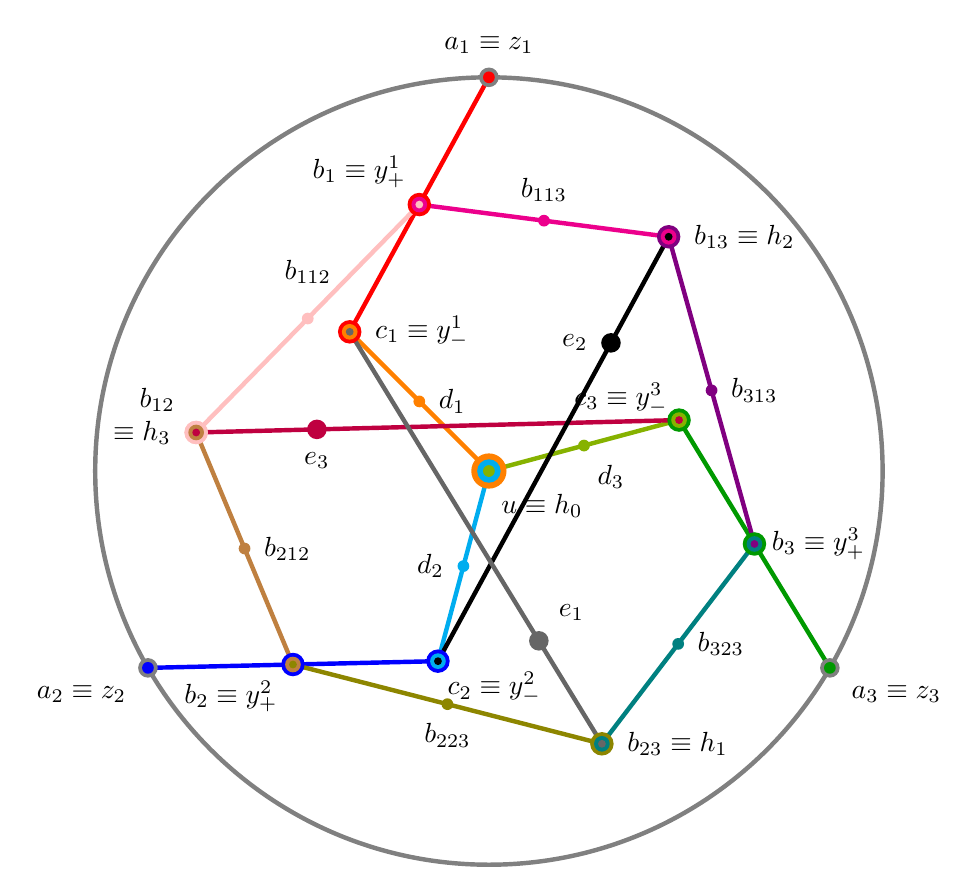
\begin{tikzpicture}[ultra thick, scale=0.5]

    % --- 1. Define all colors first for easy management ---
    \colorlet{colorCircle}{gray}
    % Colors for the three 'spokes' (a-c and c-u lines)
    \colorlet{colorAC1}{red}
    \colorlet{colorCU1}{orange}
    \colorlet{colorAC2}{blue}
    \colorlet{colorCU2}{cyan}
    \colorlet{colorAC3}{green!60!black}
    \colorlet{colorCU3}{lime!70!black}
    % Colors for the six segments of the star shape
    \colorlet{colorB1B13}{magenta}
    \colorlet{colorB13B3}{violet}
    \colorlet{colorB3B23}{teal}
    \colorlet{colorB23B2}{olive}
    \colorlet{colorB2B12}{brown}
    \colorlet{colorB12B1}{pink}
    % --- NEW: Colors for the three new connecting lines ---
    \colorlet{colorC3B12}{purple}
    \colorlet{colorC2B13}{black}   %yellow!80!
    \colorlet{colorC1B23}{black!60}


    % --- 2. Define geometric parameters ---
    \def\R{10} \def\r{5} \def\rB{7.5} \def\rD{2.5} \def\shiftangle{45}
    \def\aOneAngle{90} \def\aTwoAngle{210} \def\aThreeAngle{330}

    % --- 3. Define all coordinates without drawing the points yet ---
    \coordinate (u) at (0,0);
    \foreach \angle/\i in {\aOneAngle/1, \aTwoAngle/2, \aThreeAngle/3} {
        \coordinate (a\i) at (\angle:\R);
        \coordinate (c\i) at ({\angle+\shiftangle}:\r);
        \coordinate (d\i) at ({\angle+\shiftangle}:\rD);
    }
    \foreach \i in {1,2,3} {
        \coordinate (b\i) at ($(a\i)!0.5!(c\i)$);
    }
    \pgfmathsetmacro{\bOneAngle}{(\aOneAngle + (\aOneAngle+\shiftangle))/2}
    \pgfmathsetmacro{\bTwoAngle}{(\aTwoAngle + (\aTwoAngle+\shiftangle))/2}
    \pgfmathsetmacro{\bThreeAngle}{(\aThreeAngle + (\aThreeAngle+\shiftangle))/2}
    \pgfmathsetmacro{\bOneTwoAngle}{(\bOneAngle+\bTwoAngle)/2}
    \pgfmathsetmacro{\bTwoThreeAngle}{(\bTwoAngle+\bThreeAngle)/2}
    \pgfmathsetmacro{\bOneThreeAngle}{mod((\bThreeAngle + (\bOneAngle+360))/2, 360)}
    \coordinate (b12) at (\bOneTwoAngle:\rB);
    \coordinate (b23) at (\bTwoThreeAngle:\rB);
    \coordinate (b13) at (\bOneThreeAngle:\rB);
    \coordinate (b113) at ($(b1)!0.5!(b13)$); \coordinate (b313) at ($(b3)!0.5!(b13)$);
    \coordinate (b323) at ($(b3)!0.5!(b23)$); \coordinate (b223) at ($(b2)!0.5!(b23)$);
    \coordinate (b212) at ($(b2)!0.5!(b12)$); \coordinate (b112) at ($(b1)!0.5!(b12)$);

    % --- 4. Draw all lines with their assigned colors ---
    \draw[colorCircle] (0,0) circle (\R);
    \draw[colorAC1] (a1) -- (c1); \draw[colorCU1] (c1) -- (u);
    \draw[colorAC2] (a2) -- (c2); \draw[colorCU2] (c2) -- (u);
    \draw[colorAC3] (a3) -- (c3); \draw[colorCU3] (c3) -- (u);
    \draw[colorB1B13] (b1) -- (b13); \draw[colorB13B3] (b13) -- (b3);
    \draw[colorB3B23] (b3) -- (b23); \draw[colorB23B2] (b23) -- (b2);
    \draw[colorB2B12] (b2) -- (b12); \draw[colorB12B1] (b12) -- (b1);

    % --- NEW: Draw the three additional lines ---
    \draw[colorC3B12] (c3) -- (b12);
    \draw[colorC2B13] (c2) -- (b13);
    \draw[colorC1B23] (c1) -- (b23);

    % --- 5. Draw all points on top of the lines, with colors reflecting intersections ---
    % Points on a single line (one color)
    \node[circle, fill=colorCU1, inner sep=1.5pt, label={0:$d_1$}] at (d1) {};
    \node[circle, fill=colorCU2, inner sep=1.5pt, label={180:$d_2$}] at (d2) {};
    \node[circle, fill=colorCU3, inner sep=1.5pt, label={285:$d_3$}] at (d3) {};
    \node[circle, fill=colorB1B13, inner sep=1.5pt, label=above:$b_{113}$] at (b113) {};
    \node[circle, fill=colorB13B3, inner sep=1.5pt, label=right:$b_{313}$] at (b313) {};
    \node[circle, fill=colorB3B23, inner sep=1.5pt, label=right:$b_{323}$] at (b323) {};
    \node[circle, fill=colorB23B2, inner sep=1.5pt, label=below:$b_{223}$] at (b223) {};
    \node[circle, fill=colorB2B12, inner sep=1.5pt, label=right:$b_{212}$] at (b212) {};
    \node[circle, fill=colorB12B1, inner sep=1.5pt, label={[label distance=2mm]90:$b_{112}$}] at (b112) {};

    % Points at intersections of two lines (two colors)
    \node[circle, fill=colorCircle, inner sep=2.5pt, label={90:$a_1\equiv z_1$}] at (a1) {}; \node[circle, fill=colorAC1, inner sep=1.5pt] at (a1) {};
    \node[circle, fill=colorCircle, inner sep=2.5pt, label={210:$a_2\equiv z_2$}] at (a2) {}; \node[circle, fill=colorAC2, inner sep=1.5pt] at (a2) {};
    \node[circle, fill=colorCircle, inner sep=2.5pt, label={330:$a_3\equiv z_3$}] at (a3) {}; \node[circle, fill=colorAC3, inner sep=1.5pt] at (a3) {};

    % Points at intersections of three lines (three colors)
    % --- MODIFIED: Point u with tighter label at 275 degrees ---
    \node[circle, fill=colorCU1, inner sep=4.5pt, label={[label distance=-1mm]275:$u\equiv h_0$}] at (u) {};
    \node[circle, fill=colorCU2, inner sep=3pt] at (u) {};
    \node[circle, fill=colorCU3, inner sep=1.5pt] at (u) {};
    \node[circle, fill=colorAC1, inner sep=3pt, label={[label distance=-1mm]110:$b_1\equiv y_+^1$}] at (b1) {}; \node[circle, fill=colorB1B13, inner sep=2pt] at (b1) {}; \node[circle, fill=colorB12B1, inner sep=1pt] at (b1) {};
    \node[circle, fill=colorAC2, inner sep=3pt, label={[label distance=-1mm]230:$b_2\equiv y_+^2$}] at (b2) {}; \node[circle, fill=colorB2B12, inner sep=2pt] at (b2) {}; \node[circle, fill=colorB23B2, inner sep=1pt] at (b2) {};
    \node[circle, fill=colorAC3, inner sep=3pt, label={[label distance=-1mm]0:$b_3\equiv y_+^3$}] at (b3) {}; \node[circle, fill=colorB3B23, inner sep=2pt] at (b3) {}; \node[circle, fill=colorB13B3, inner sep=1pt] at (b3) {};

    % --- UPDATED: These points are now intersections of THREE lines ---
    \node[circle, fill=colorAC1, inner sep=3pt, label={0:$c_1\equiv y_-^1$}] at (c1) {}; \node[circle, fill=colorCU1, inner sep=2pt] at (c1) {}; \node[circle, fill=colorC1B23, inner sep=1pt] at (c1) {};
    \node[circle, fill=colorAC2, inner sep=3pt, label={[label distance=-2mm]-5:$c_2\equiv y_-^2$}] at (c2) {}; \node[circle, fill=colorCU2, inner sep=2pt] at (c2) {}; \node[circle, fill=colorC2B13, inner sep=1pt] at (c2) {};
    \node[circle, fill=colorAC3, inner sep=3pt, label={[label distance=-2.5mm]93:$c_3\equiv y_-^3$}] at (c3) {}; \node[circle, fill=colorCU3, inner sep=2pt] at (c3) {}; \node[circle, fill=colorC3B12, inner sep=1pt] at (c3) {};

    \node[circle, fill=colorB12B1, inner sep=3pt, label={above left:$b_{12}$}] at (b12) {};
    \node[circle, fill=colorB12B1, inner sep=3pt, label={left:$\equiv h_3$}] at (b12) {};
    \node[circle, fill=colorB2B12, inner sep=2pt] at (b12) {}; \node[circle, fill=colorC3B12, inner sep=1pt] at (b12) {};
    \node[circle, fill=colorB23B2, inner sep=3pt, label=right:$b_{23}\equiv h_1$] at (b23) {}; \node[circle, fill=colorB3B23, inner sep=2pt] at (b23) {}; \node[circle, fill=colorC1B23, inner sep=1pt] at (b23) {};
    \node[circle, fill=colorB13B3, inner sep=3pt, label=right:$b_{13}\equiv h_2$] at (b13) {}; \node[circle, fill=colorB1B13, inner sep=2pt] at (b13) {}; \node[circle, fill=colorC2B13, inner sep=1pt] at (b13) {};

% --- NEW: Add the three e_i points ---
    % e_1 is placed 3/4 of the way along the line from c1 to b23
    \node[circle, fill=colorC1B23, inner sep=2.5pt, label={above right:$e_1$}] (e1) at ($(c1)!0.75!(b23)$) {};

    % e_2 is placed 3/4 of the way along the line from c2 to b13
    \node[circle, fill=colorC2B13, inner sep=2.5pt, label={left:$e_2$}] (e2) at ($(c2)!0.75!(b13)$) {};

    % e_3 is placed 3/4 of the way along the line from c3 to b12
    \node[circle, fill=colorC3B12, inner sep=2.5pt, label={below:$e_3$}] (e3) at ($(c3)!0.75!(b12)$) {};

\end{tikzpicture}
}
\caption{The Yu-Oh quantum logic~\cite{Yu-2012} drawn in the Harding and Salinas Schmeis 3-uniform hypergraph scheme~\cite{harding2025remarksIJTP}.}
\label{fig:yohs}
\end{figure}


\begin{table*}[htbp]
\caption{\label{tab:vector_generation}
\textit{Systematic generation of the vector set for contextuality analysis.}
This table details the complete set of 225 vectors that form the basis of our structural analysis.
A family of 25 algebraic functions (rows) is applied to nine initial vectors (columns $u_1$--$u_9$).
These initial vectors comprise all three MUBs in $\mathbb{C}^3$:
the Fourier basis $\mathcal{B}_1 = \{u_1, u_2, u_3\}$,
and two related MUBs,
$\mathcal{B}_2 = \{u_4, u_5, u_6\}$ and its complex conjugate $\mathcal{B}_3 = \{u_7, u_8, u_9\}$; all yielding 69-50 KS sets.
The final column counts the number of unique rays produced by each function,
highlighting the differing projective variety of the constructions.
The 165 unique rays drawn from this set form the labels for identifying orthogonal bases, hyperedges, or contexts.
Labelling according to the Harding and Salinas Schmeis scheme~\cite{harding2025remarksIJTP};
with equivalences to the Yu-Oh numbering scheme~\cite{Yu-2012}.
}
\begin{ruledtabular}
\begin{tabular}{ccccccccccc}
basis&
      \multicolumn{3}{c|}{$\mathcal{B}_1$}&
      \multicolumn{3}{c|}{$\mathcal{B}_2$}&
      \multicolumn{3}{c}{$\mathcal{B}_3$}\\
\hline
label & $u_{1}$ & $u_{2}$ & $u_{3}$ & $u_{4}$ & $u_{5}$ & $u_{6}$ & $u_{7}$ & $u_{8}$ & $u_{9}$ & \#  \\ \hline
$a_1\equiv z_1$ & $(1,0,0)$ & $(1,0,0)$ & $(1,0,0)$ & $(1,0,0)$ & $(1,0,0)$ & $(1,0,0)$ & $(1,0,0)$ & $(1,0,0)$ & $(1,0,0)$ & 1 \\
$a_2\equiv z_2$ & $(0,1,0)$ & $(0,1,0)$ & $(0,1,0)$ & $(0,1,0)$ & $(0,1,0)$ & $(0,1,0)$ & $(0,1,0)$ & $(0,1,0)$ & $(0,1,0)$ & 1 \\
$a_3\equiv z_3$ & $(0,0,1)$ & $(0,0,1)$ & $(0,0,1)$ & $(0,0,1)$ & $(0,0,1)$ & $(0,0,1)$ & $(0,0,1)$ & $(0,0,1)$ & $(0,0,1)$ & 1 \\
$u\equiv h_0$ & $(1,1,1)$ & $(1,\omega,\omega^2)$ & $(1,\omega^2,\omega)$ & $(1,\omega,\omega)$ & $(1,\omega^2,1)$ & $(1,1,\omega^2)$ & $(1,\omega^2,\omega^2)$ & $(1,\omega,1)$ & $(1,1,\omega)$ & 9 \\
$b_1\equiv y_+^1$ & $(0,1,1)$ & $(0,\omega,\omega^2)$ & $(0,\omega^2,\omega)$ & $(0,\omega,\omega)$ & $(0,\omega^2,1)$ & $(0,1,\omega^2)$ & $(0,\omega^2,\omega^2)$ & $(0,\omega,1)$ & $(0,1,\omega)$ & 3 \\
$b_2\equiv y_+^2$ & $(1,0,1)$ & $(1,0,\omega^2)$ & $(1,0,\omega)$ & $(1,0,\omega)$ & $(1,0,1)$ & $(1,0,\omega^2)$ & $(1,0,\omega^2)$ & $(1,0,1)$ & $(1,0,\omega)$ & 3 \\
$b_3\equiv y_+^3$ & $(1,1,0)$ & $(1,\omega,0)$ & $(1,\omega^2,0)$ & $(1,\omega,0)$ & $(1,\omega^2,0)$ & $(1,1,0)$ & $(1,\omega^2,0)$ & $(1,\omega,0)$ & $(1,1,0)$ & 3 \\
$c_1\equiv y_-^1$ & $(0,1,-1)$ & $(0,\omega,-\omega^2)$ & $(0,\omega^2,-\omega)$ & $(0,\omega^2,-\omega^2)$ & $(0,1,-\omega)$ & $(0,\omega,-1)$ & $(0,\omega,-\omega)$ & $(0,1,-\omega^2)$ & $(0,\omega^2,-1)$ & 3 \\
$c_2\equiv y_-^2$ & $(-1,0,1)$ & $(-\omega,0,1)$ & $(-\omega^2,0,1)$ & $(-\omega^2,0,1)$ & $(-1,0,1)$ & $(-\omega,0,1)$ & $(-\omega,0,1)$ & $(-1,0,1)$ & $(-\omega^2,0,1)$ & 3 \\
$c_3\equiv y_-^3$ & $(1,-1,0)$ & $(\omega^2,-1,0)$ & $(\omega,-1,0)$ & $(\omega^2,-1,0)$ & $(\omega,-1,0)$ & $(1,-1,0)$ & $(\omega,-1,0)$ & $(\omega^2,-1,0)$ & $(1,-1,0)$ & 3 \\
$d_1$ & $(-2,1,1)$ & $(-2,\omega,\omega^2)$ & $(-2,\omega^2,\omega)$ & $(-2,\omega,\omega)$ & $(-2,\omega^2,1)$ & $(-2,1,\omega^2)$ & $(-2,\omega^2,\omega^2)$ & $(-2,\omega,1)$ & $(-2,1,\omega)$ & 9 \\
$d_2$ & $(1,-2,1)$ & $(\omega^2,-2,\omega)$ & $(\omega,-2,\omega^2)$ & $(\omega^2,-2,1)$ & $(\omega,-2,\omega)$ & $(1,-2,\omega^2)$ & $(\omega,-2,1)$ & $(\omega^2,-2,\omega^2)$ & $(1,-2,\omega)$ & 9 \\
$d_3$ & $(1,1,-2)$ & $(\omega,\omega^2,-2)$ & $(\omega^2,\omega,-2)$ & $(\omega^2,1,-2)$ & $(1,\omega^2,-2)$ & $(\omega,\omega,-2)$ & $(\omega,1,-2)$ & $(1,\omega,-2)$ & $(\omega^2,\omega^2,-2)$ & 9 \\
$b_{12}\equiv h_3$ & $(1,1,-1)$ & $(1,\omega,-\omega^2)$ & $(1,\omega^2,-\omega)$ & $(\omega,\omega^2,-\omega^2)$ & $(\omega,1,-\omega)$ & $(\omega,\omega,-1)$ & $(\omega^2,\omega,-\omega)$ & $(\omega^2,1,-\omega^2)$ & $(\omega^2,\omega^2,-1)$ & 9 \\
$b_{13}\equiv h_2$ & $(1,-1,1)$ & $(1,-\omega,\omega^2)$ & $(1,-\omega^2,\omega)$ & $(\omega,-\omega^2,\omega^2)$ & $(\omega,-1,\omega)$ & $(\omega,-\omega,1)$ & $(\omega^2,-\omega,\omega)$ & $(\omega^2,-1,\omega^2)$ & $(\omega^2,-\omega^2,1)$ & 9 \\
$b_{23}\equiv h_1$ & $(-1,1,1)$ & $(-1,\omega,\omega^2)$ & $(-1,\omega^2,\omega)$ & $(-\omega,\omega^2,\omega^2)$ & $(-\omega,1,\omega)$ & $(-\omega,\omega,1)$ & $(-\omega^2,\omega,\omega)$ & $(-\omega^2,1,\omega^2)$ & $(-\omega^2,\omega^2,1)$ & 9 \\
$e_1$ & $(1,2,1)$ & $(\omega^2,2,\omega)$ & $(\omega,2,\omega^2)$ & $(\omega,2\omega^2,\omega^2)$ & $(1,2\omega^2,1)$ & $(\omega^2,2\omega^2,\omega)$ & $(\omega^2,2\omega,\omega)$ & $(1,2\omega,1)$ & $(\omega,2\omega,\omega^2)$ & 9 \\
$e_2$ & $(1,1,2)$ & $(\omega,\omega^2,2)$ & $(\omega^2,\omega,2)$ & $(\omega,\omega^2,2\omega^2)$ & $(\omega^2,\omega,2\omega^2)$ & $(1,1,2\omega^2)$ & $(\omega^2,\omega,2\omega)$ & $(\omega,\omega^2,2\omega)$ & $(1,1,2\omega)$ & 9 \\
$e_3$ & $(2,1,1)$ & $(2,\omega,\omega^2)$ & $(2,\omega^2,\omega)$ & $(2\omega^2,1,1)$ & $(2\omega^2,\omega,\omega^2)$ & $(2\omega^2,\omega^2,\omega)$ & $(2\omega,1,1)$ & $(2\omega,\omega^2,\omega)$ & $(2\omega,\omega,\omega^2)$ & 9 \\
$b_{112}$ & $(2,-1,1)$ & $(2,-\omega,\omega^2)$ & $(2,-\omega^2,\omega)$ & $(2,-\omega,\omega)$ & $(2,-\omega^2,1)$ & $(2,-1,\omega^2)$ & $(2,-\omega^2,\omega^2)$ & $(2,-\omega,1)$ & $(2,-1,\omega)$ & 9 \\
$b_{212}$ & $(-1,2,1)$ & $(-1,2\omega,\omega^2)$ & $(-1,2\omega^2,\omega)$ & $(-1,2\omega,\omega)$ & $(-1,2\omega^2,1)$ & $(-1,2,\omega^2)$ & $(-1,2\omega^2,\omega^2)$ & $(-1,2\omega,1)$ & $(-1,2,\omega)$ & 9 \\
$b_{113}$ & $(2,1,-1)$ & $(2,\omega,-\omega^2)$ & $(2,\omega^2,-\omega)$ & $(2,\omega,-\omega)$ & $(2,\omega^2,-1)$ & $(2,1,-\omega^2)$ & $(2,\omega^2,-\omega^2)$ & $(2,\omega,-1)$ & $(2,1,-\omega)$ & 9 \\
$b_{313}$ & $(-1,1,2)$ & $(-1,\omega,2\omega^2)$ & $(-1,\omega^2,2\omega)$ & $(-1,\omega,2\omega)$ & $(-1,\omega^2,2)$ & $(-1,1,2\omega^2)$ & $(-1,\omega^2,2\omega^2)$ & $(-1,\omega,2)$ & $(-1,1,2\omega)$ & 9 \\
$b_{223}$ & $(1,2,-1)$ & $(1,2\omega,-\omega^2)$ & $(1,2\omega^2,-\omega)$ & $(1,2\omega,-\omega)$ & $(1,2\omega^2,-1)$ & $(1,2,-\omega^2)$ & $(1,2\omega^2,-\omega^2)$ & $(1,2\omega,-1)$ & $(1,2,-\omega)$ & 9 \\
$b_{323}$ & $(1,-1,2)$ & $(1,-\omega,2\omega^2)$ & $(1,-\omega^2,2\omega)$ & $(1,-\omega,2\omega)$ & $(1,-\omega^2,2)$ & $(1,-1,2\omega^2)$ & $(1,-\omega^2,2\omega^2)$ & $(1,-\omega,2)$ & $(1,-1,2\omega)$ & 9 \\
\end{tabular}
\end{ruledtabular}
\end{table*}



\subsection{Total Number of Globally Non-Collinear Vectors: 165}

A total of 165 unique, non-collinear vectors were identified from the analysis of the nine fundamental vectors $u_1$ through $u_9$
in Table~\ref{tab:vector_generation}.
These vectors, which form the basis for constructing orthogonal triples, are enumerated in Table~\ref{tab:noncollinear_vectors_6col}.
The coordinate system is based on the complex third root of unity, $\omega = e^{2\pi i/3}$.

This vector set is not closed with respect to the complex ``cross product''~\cite{harding2025remarksIJTP} (sometimes referred to as Hermitian cross product)
\(
u\times v =  (\overline{u_2v_3-u_3v_2},\overline{u_3v_1-u_1v_3},\overline{u_1v_2-u_2v_1})
\)
of two vectors $u=(u_1,u_2,u_3)$ and $v=(v_1,v_2,v_3)$ in $\mathbb{R}^3$ or $\mathbb{C}^3$ because, say,
$a_1 \times d_{21} = (1,0,0) \times (1,-2,1) = -(0,1,2)$, which is not collinear with any vector of the set of globally non-collinear vectors.



\begin{table*}[htbp!]
\caption{
The complete set of 165 globally unique non-collinear vectors, with six entries per row.
The right index (such as $j$ in $u_j$) refers to the column index (shifted by $-1$) in Table~\ref{tab:vector_generation}.
The color coding indicates the fundamental set from which each vector is derived.
\textcolor{red}{Red vectors} originate exclusively from the set $\mathcal{B}_1=\{u_1, u_2, u_3\}$.
\textcolor{green}{Green vectors} originate exclusively from $\mathcal{B}_2=\{u_4, u_5, u_6\}$.
\textcolor{blue}{Blue vectors} originate exclusively from $\mathcal{B}_3=\{u_7, u_8, u_9\}$.
The standard Cartesian basis vectors  $a_{11}$, $a_{21}$, and $a_{31}$  are shown in black, as they are
(the only) ``universal'' or ``global'' vectors contained in the vector sets derived from all three fundamental MUBs.
}
\label{tab:noncollinear_vectors_6col}
\footnotesize % Use a smaller font to fit the content
\begin{ruledtabular}
\begin{tabular}{*{6}{c}} % 6 centered columns
{$a_{11}=(1,0,0)$} & {$a_{21}=(0,1,0)$} & {$a_{31}=(0,0,1)$} & \textcolor{red}{$u_{1}=(1,1,1)$} & \textcolor{red}{$u_{2}=(1,\omega,\omega^2)$} & \textcolor{red}{$u_{3}=(1,\omega^2,\omega)$} \\
\textcolor{green}{$u_{4}=(1,\omega,\omega)$} & \textcolor{green}{$u_{5}=(1,\omega^2,1)$} & \textcolor{green}{$u_{6}=(1,1,\omega^2)$} & \textcolor{blue}{$u_{7}=(1,\omega^2,\omega^2)$} & \textcolor{blue}{$u_{8}=(1,\omega,1)$} & \textcolor{blue}{$u_{9}=(1,1,\omega)$} \\
\textcolor{red}{$b_{11}=(0,1,1)$} & \textcolor{red}{$b_{12}=(0,\omega,\omega^2)$} & \textcolor{red}{$b_{13}=(0,\omega^2,\omega)$} & \textcolor{red}{$b_{21}=(1,0,1)$} & \textcolor{red}{$b_{22}=(1,0,\omega^2)$} & \textcolor{red}{$b_{23}=(1,0,\omega)$} \\
\textcolor{red}{$b_{31}=(1,1,0)$} & \textcolor{red}{$b_{32}=(1,\omega,0)$} & \textcolor{red}{$b_{33}=(1,\omega^2,0)$} & \textcolor{red}{$c_{11}=(0,1,-1)$} & \textcolor{red}{$c_{12}=(0,\omega,-\omega^2)$} & \textcolor{red}{$c_{13}=(0,\omega^2,-\omega)$} \\
\textcolor{red}{$c_{21}=(-1,0,1)$} & \textcolor{red}{$c_{22}=(-\omega,0,1)$} & \textcolor{red}{$c_{23}=(-\omega^2,0,1)$} & \textcolor{red}{$c_{31}=(1,-1,0)$} & \textcolor{red}{$c_{32}=(\omega^2,-1,0)$} & \textcolor{red}{$c_{33}=(\omega,-1,0)$} \\
\textcolor{red}{$d_{11}=(-2,1,1)$} & \textcolor{red}{$d_{12}=(-2,\omega,\omega^2)$} & \textcolor{red}{$d_{13}=(-2,\omega^2,\omega)$} & \textcolor{green}{$d_{14}=(-2,\omega,\omega)$} & \textcolor{green}{$d_{15}=(-2,\omega^2,1)$} & \textcolor{green}{$d_{16}=(-2,1,\omega^2)$} \\
\textcolor{blue}{$d_{17}=(-2,\omega^2,\omega^2)$} & \textcolor{blue}{$d_{18}=(-2,\omega,1)$} & \textcolor{blue}{$d_{19}=(-2,1,\omega)$} & \textcolor{red}{$d_{21}=(1,-2,1)$} & \textcolor{red}{$d_{22}=(\omega^2,-2,\omega)$} & \textcolor{red}{$d_{23}=(\omega,-2,\omega^2)$} \\
\textcolor{green}{$d_{24}=(\omega^2,-2,1)$} & \textcolor{green}{$d_{25}=(\omega,-2,\omega)$} & \textcolor{green}{$d_{26}=(1,-2,\omega^2)$} & \textcolor{blue}{$d_{27}=(\omega,-2,1)$} & \textcolor{blue}{$d_{28}=(\omega^2,-2,\omega^2)$} & \textcolor{blue}{$d_{29}=(1,-2,\omega)$} \\
\textcolor{red}{$d_{31}=(1,1,-2)$} & \textcolor{red}{$d_{32}=(\omega,\omega^2,-2)$} & \textcolor{red}{$d_{33}=(\omega^2,\omega,-2)$} & \textcolor{green}{$d_{34}=(\omega^2,1,-2)$} & \textcolor{green}{$d_{35}=(1,\omega^2,-2)$} & \textcolor{green}{$d_{36}=(\omega,\omega,-2)$} \\
\textcolor{blue}{$d_{37}=(\omega,1,-2)$} & \textcolor{blue}{$d_{38}=(1,\omega,-2)$} & \textcolor{blue}{$d_{39}=(\omega^2,\omega^2,-2)$} & \textcolor{red}{$b_{121}=(1,1,-1)$} & \textcolor{red}{$b_{122}=(1,\omega,-\omega^2)$} & \textcolor{red}{$b_{123}=(1,\omega^2,-\omega)$} \\
\textcolor{green}{$b_{124}=(\omega,\omega^2,-\omega^2)$} & \textcolor{green}{$b_{125}=(\omega,1,-\omega)$} & \textcolor{green}{$b_{126}=(\omega,\omega,-1)$} & \textcolor{blue}{$b_{127}=(\omega^2,\omega,-\omega)$} & \textcolor{blue}{$b_{128}=(\omega^2,1,-\omega^2)$} & \textcolor{blue}{$b_{129}=(\omega^2,\omega^2,-1)$} \\
\textcolor{red}{$b_{131}=(1,-1,1)$} & \textcolor{red}{$b_{132}=(1,-\omega,\omega^2)$} & \textcolor{red}{$b_{133}=(1,-\omega^2,\omega)$} & \textcolor{green}{$b_{134}=(\omega,-\omega^2,\omega^2)$} & \textcolor{green}{$b_{135}=(\omega,-1,\omega)$} & \textcolor{green}{$b_{136}=(\omega,-\omega,1)$} \\
\textcolor{blue}{$b_{137}=(\omega^2,-\omega,\omega)$} & \textcolor{blue}{$b_{138}=(\omega^2,-1,\omega^2)$} & \textcolor{blue}{$b_{139}=(\omega^2,-\omega^2,1)$} & \textcolor{red}{$b_{231}=(-1,1,1)$} & \textcolor{red}{$b_{232}=(-1,\omega,\omega^2)$} & \textcolor{red}{$b_{233}=(-1,\omega^2,\omega)$} \\
\textcolor{green}{$b_{234}=(-\omega,\omega^2,\omega^2)$} & \textcolor{green}{$b_{235}=(-\omega,1,\omega)$} & \textcolor{green}{$b_{236}=(-\omega,\omega,1)$} & \textcolor{blue}{$b_{237}=(-\omega^2,\omega,\omega)$} & \textcolor{blue}{$b_{238}=(-\omega^2,1,\omega^2)$} & \textcolor{blue}{$b_{239}=(-\omega^2,\omega^2,1)$} \\
\textcolor{red}{$e_{11}=(1,2,1)$} & \textcolor{red}{$e_{12}=(\omega^2,2,\omega)$} & \textcolor{red}{$e_{13}=(\omega,2,\omega^2)$} & \textcolor{green}{$e_{14}=(\omega,2\omega^2,\omega^2)$} & \textcolor{green}{$e_{15}=(1,2\omega^2,1)$} & \textcolor{green}{$e_{16}=(\omega^2,2\omega^2,\omega)$} \\
\textcolor{blue}{$e_{17}=(\omega^2,2\omega,\omega)$} & \textcolor{blue}{$e_{18}=(1,2\omega,1)$} & \textcolor{blue}{$e_{19}=(\omega,2\omega,\omega^2)$} & \textcolor{red}{$e_{21}=(1,1,2)$} & \textcolor{red}{$e_{22}=(\omega,\omega^2,2)$} & \textcolor{red}{$e_{23}=(\omega^2,\omega,2)$} \\
\textcolor{green}{$e_{24}=(\omega,\omega^2,2\omega^2)$} & \textcolor{green}{$e_{25}=(\omega^2,\omega,2\omega^2)$} & \textcolor{green}{$e_{26}=(1,1,2\omega^2)$} & \textcolor{blue}{$e_{27}=(\omega^2,\omega,2\omega)$} & \textcolor{blue}{$e_{28}=(\omega,\omega^2,2\omega)$} & \textcolor{blue}{$e_{29}=(1,1,2\omega)$} \\
\textcolor{red}{$e_{31}=(2,1,1)$} & \textcolor{red}{$e_{32}=(2,\omega,\omega^2)$} & \textcolor{red}{$e_{33}=(2,\omega^2,\omega)$} & \textcolor{green}{$e_{34}=(2\omega^2,1,1)$} & \textcolor{green}{$e_{35}=(2\omega^2,\omega,\omega^2)$} & \textcolor{green}{$e_{36}=(2\omega^2,\omega^2,\omega)$} \\
\textcolor{blue}{$e_{37}=(2\omega,1,1)$} & \textcolor{blue}{$e_{38}=(2\omega,\omega^2,\omega)$} & \textcolor{blue}{$e_{39}=(2\omega,\omega,\omega^2)$} & \textcolor{red}{$b_{1121}=(2,-1,1)$} & \textcolor{red}{$b_{1122}=(2,-\omega,\omega^2)$} & \textcolor{red}{$b_{1123}=(2,-\omega^2,\omega)$} \\
\textcolor{green}{$b_{1124}=(2,-\omega,\omega)$} & \textcolor{green}{$b_{1125}=(2,-\omega^2,1)$} & \textcolor{green}{$b_{1126}=(2,-1,\omega^2)$} & \textcolor{blue}{$b_{1127}=(2,-\omega^2,\omega^2)$} & \textcolor{blue}{$b_{1128}=(2,-\omega,1)$} & \textcolor{blue}{$b_{1129}=(2,-1,\omega)$} \\
\textcolor{red}{$b_{2121}=(-1,2,1)$} & \textcolor{red}{$b_{2122}=(-1,2\omega,\omega^2)$} & \textcolor{red}{$b_{2123}=(-1,2\omega^2,\omega)$} & \textcolor{green}{$b_{2124}=(-1,2\omega,\omega)$} & \textcolor{green}{$b_{2125}=(-1,2\omega^2,1)$} & \textcolor{green}{$b_{2126}=(-1,2,\omega^2)$} \\
\textcolor{blue}{$b_{2127}=(-1,2\omega^2,\omega^2)$} & \textcolor{blue}{$b_{2128}=(-1,2\omega,1)$} & \textcolor{blue}{$b_{2129}=(-1,2,\omega)$} & \textcolor{red}{$b_{1131}=(2,1,-1)$} & \textcolor{red}{$b_{1132}=(2,\omega,-\omega^2)$} & \textcolor{red}{$b_{1133}=(2,\omega^2,-\omega)$} \\
\textcolor{green}{$b_{1134}=(2,\omega,-\omega)$} & \textcolor{green}{$b_{1135}=(2,\omega^2,-1)$} & \textcolor{green}{$b_{1136}=(2,1,-\omega^2)$} & \textcolor{blue}{$b_{1137}=(2,\omega^2,-\omega^2)$} & \textcolor{blue}{$b_{1138}=(2,\omega,-1)$} & \textcolor{blue}{$b_{1139}=(2,1,-\omega)$} \\
\textcolor{red}{$b_{3131}=(-1,1,2)$} & \textcolor{red}{$b_{3132}=(-1,\omega,2\omega^2)$} & \textcolor{red}{$b_{3133}=(-1,\omega^2,2\omega)$} & \textcolor{green}{$b_{3134}=(-1,\omega,2\omega)$} & \textcolor{green}{$b_{3135}=(-1,\omega^2,2)$} & \textcolor{green}{$b_{3136}=(-1,1,2\omega^2)$} \\
\textcolor{blue}{$b_{3137}=(-1,\omega^2,2\omega^2)$} & \textcolor{blue}{$b_{3138}=(-1,\omega,2)$} & \textcolor{blue}{$b_{3139}=(-1,1,2\omega)$} & \textcolor{red}{$b_{2231}=(1,2,-1)$} & \textcolor{red}{$b_{2232}=(1,2\omega,-\omega^2)$} & \textcolor{red}{$b_{2233}=(1,2\omega^2,-\omega)$} \\
\textcolor{green}{$b_{2234}=(1,2\omega,-\omega)$} & \textcolor{green}{$b_{2235}=(1,2\omega^2,-1)$} & \textcolor{green}{$b_{2236}=(1,2,-\omega^2)$} & \textcolor{blue}{$b_{2237}=(1,2\omega^2,-\omega^2)$} & \textcolor{blue}{$b_{2238}=(1,2\omega,-1)$} & \textcolor{blue}{$b_{2239}=(1,2,-\omega)$} \\
\textcolor{red}{$b_{3231}=(1,-1,2)$} & \textcolor{red}{$b_{3232}=(1,-\omega,2\omega^2)$} & \textcolor{red}{$b_{3233}=(1,-\omega^2,2\omega)$} & \textcolor{green}{$b_{3234}=(1,-\omega,2\omega)$} & \textcolor{green}{$b_{3235}=(1,-\omega^2,2)$} & \textcolor{green}{$b_{3236}=(1,-1,2\omega^2)$} \\
\textcolor{blue}{$b_{3237}=(1,-\omega^2,2\omega^2)$} & \textcolor{blue}{$b_{3238}=(1,-\omega,2)$} & \textcolor{blue}{$b_{3239}=(1,-1,2\omega)$} & & & \\
\end{tabular}
\end{ruledtabular}
\end{table*}

\subsection{Total number of orthogonal bases: 130}


\begin{table*}[htbp!]
\caption{
A comprehensive list of the 130 orthogonal bases, color-coded according to the exclusive origin of their constituent vectors.
The coloring follows a strict hierarchy:
Individual vectors are considered ``pure'' (\textcolor{red}{red}, \textcolor{green}{green}, or \textcolor{blue}{blue})
if they originate exclusively from a single fundamental set.
Vectors derivable from multiple sets, like the standard basis \{$a_{11}, a_{21}, a_{31}$\}, are ``universal'' and thus black.
A basis is colored in \textcolor{red}{red}, \textcolor{green}{green}, or \textcolor{blue}{blue} if and only if it is composed of three vectors
of the \textit{same pure color}.
All other bases are classified as ``mixed'' and thus black.
This includes bases with vectors of different pure colors and any basis containing one or more universal vectors.
According to Table~\ref{tab:vector_generation}, the only ``universal'' or ``global'' vectors contained
in the vector sets derived from all three fundamental MUBs are the three standard Cartesian basis vectors:
$a_{11}=(1,0,0)$, $a_{21}=(0,1,0)$, and $a_{31}=(0,0,1)$.
}
\label{tab:orthogonal_bases}
\begin{ruledtabular}
\begin{tabular}{ccccccc} %

% --- Table Content (6 bases per row) ---
{\{$a_{11}$, $a_{21}$, $a_{31}$\}} & {\{$a_{11}$, $b_{11}$, $c_{11}$\}} & {\{$a_{11}$, $b_{12}$, $c_{12}$\}} & {\{$a_{11}$, $b_{13}$, $c_{13}$\}} & {\{$a_{21}$, $b_{21}$, $c_{21}$\}} & {\{$a_{21}$, $b_{22}$, $c_{22}$\}} \\
{\{$a_{21}$, $b_{23}$, $c_{23}$\}} & {\{$a_{31}$, $b_{31}$, $c_{31}$\}} & {\{$a_{31}$, $b_{32}$, $c_{32}$\}} & {\{$a_{31}$, $b_{33}$, $c_{33}$\}} & \textcolor{red}{\{$u_{1}$, $u_{2}$, $u_{3}$\}} & \textcolor{red}{\{$u_{1}$, $c_{11}$, $d_{11}$\}} \\
\textcolor{red}{\{$u_{1}$, $c_{21}$, $d_{21}$\}} & \textcolor{red}{\{$u_{1}$, $c_{31}$, $d_{31}$\}} & \textcolor{red}{\{$u_{2}$, $c_{12}$, $d_{12}$\}} & \textcolor{red}{\{$u_{2}$, $c_{22}$, $d_{22}$\}} & \textcolor{red}{\{$u_{2}$, $c_{32}$, $d_{32}$\}} & \textcolor{red}{\{$u_{3}$, $c_{13}$, $d_{13}$\}} \\
\textcolor{red}{\{$u_{3}$, $c_{23}$, $d_{23}$\}} & \textcolor{red}{\{$u_{3}$, $c_{33}$, $d_{33}$\}} & \textcolor{green}{\{$u_{4}$, $u_{5}$, $u_{6}$\}} & \{$u_{4}$, $c_{11}$, $d_{14}$\} & \{$u_{4}$, $c_{23}$, $d_{24}$\} & \{$u_{4}$, $c_{32}$, $d_{34}$\} \\
\{$u_{5}$, $c_{12}$, $d_{15}$\} & \{$u_{5}$, $c_{21}$, $d_{25}$\} & \{$u_{5}$, $c_{33}$, $d_{35}$\} & \{$u_{6}$, $c_{13}$, $d_{16}$\} & \{$u_{6}$, $c_{22}$, $d_{26}$\} & \{$u_{6}$, $c_{31}$, $d_{36}$\} \\
\textcolor{blue}{\{$u_{7}$, $u_{8}$, $u_{9}$\}} & \{$u_{7}$, $c_{11}$, $d_{17}$\} & \{$u_{7}$, $c_{22}$, $d_{27}$\} & \{$u_{7}$, $c_{33}$, $d_{37}$\} & \{$u_{8}$, $c_{13}$, $d_{18}$\} & \{$u_{8}$, $c_{21}$, $d_{28}$\} \\
\{$u_{8}$, $c_{32}$, $d_{38}$\} & \{$u_{9}$, $c_{12}$, $d_{19}$\} & \{$u_{9}$, $c_{23}$, $d_{29}$\} & \{$u_{9}$, $c_{31}$, $d_{39}$\} & \textcolor{red}{\{$b_{11}$, $b_{121}$, $b_{1121}$\}} & \{$b_{11}$, $b_{124}$, $b_{1124}$\} \\
\{$b_{11}$, $b_{127}$, $b_{1127}$\} & \textcolor{red}{\{$b_{11}$, $b_{131}$, $b_{1131}$\}} & \{$b_{11}$, $b_{134}$, $b_{1134}$\} & \{$b_{11}$, $b_{137}$, $b_{1137}$\} & \textcolor{red}{\{$b_{12}$, $b_{122}$, $b_{1122}$\}} & \{$b_{12}$, $b_{125}$, $b_{1125}$\} \\
\{$b_{12}$, $b_{129}$, $b_{1129}$\} & \textcolor{red}{\{$b_{12}$, $b_{132}$, $b_{1132}$\}} & \{$b_{12}$, $b_{135}$, $b_{1135}$\} & \{$b_{12}$, $b_{139}$, $b_{1139}$\} & \textcolor{red}{\{$b_{13}$, $b_{123}$, $b_{1123}$\}} & \{$b_{13}$, $b_{126}$, $b_{1126}$\} \\
\{$b_{13}$, $b_{128}$, $b_{1128}$\} & \textcolor{red}{\{$b_{13}$, $b_{133}$, $b_{1133}$\}} & \{$b_{13}$, $b_{136}$, $b_{1136}$\} & \{$b_{13}$, $b_{138}$, $b_{1138}$\} & \textcolor{red}{\{$b_{21}$, $b_{121}$, $b_{2121}$\}} & \{$b_{21}$, $b_{125}$, $b_{2125}$\} \\
\{$b_{21}$, $b_{128}$, $b_{2128}$\} & \textcolor{red}{\{$b_{21}$, $b_{231}$, $b_{2231}$\}} & \{$b_{21}$, $b_{235}$, $b_{2235}$\} & \{$b_{21}$, $b_{238}$, $b_{2238}$\} & \textcolor{red}{\{$b_{22}$, $b_{122}$, $b_{2122}$\}} & \{$b_{22}$, $b_{126}$, $b_{2126}$\} \\
\{$b_{22}$, $b_{127}$, $b_{2127}$\} & \textcolor{red}{\{$b_{22}$, $b_{232}$, $b_{2232}$\}} & \{$b_{22}$, $b_{236}$, $b_{2236}$\} & \{$b_{22}$, $b_{237}$, $b_{2237}$\} & \textcolor{red}{\{$b_{23}$, $b_{123}$, $b_{2123}$\}} & \{$b_{23}$, $b_{124}$, $b_{2124}$\} \\
\{$b_{23}$, $b_{129}$, $b_{2129}$\} & \textcolor{red}{\{$b_{23}$, $b_{233}$, $b_{2233}$\}} & \{$b_{23}$, $b_{234}$, $b_{2234}$\} & \{$b_{23}$, $b_{239}$, $b_{2239}$\} & \textcolor{red}{\{$b_{31}$, $b_{131}$, $b_{3131}$\}} & \{$b_{31}$, $b_{136}$, $b_{3136}$\} \\
\{$b_{31}$, $b_{139}$, $b_{3139}$\} & \textcolor{red}{\{$b_{31}$, $b_{231}$, $b_{3231}$\}} & \{$b_{31}$, $b_{236}$, $b_{3236}$\} & \{$b_{31}$, $b_{239}$, $b_{3239}$\} & \textcolor{red}{\{$b_{32}$, $b_{132}$, $b_{3132}$\}} & \{$b_{32}$, $b_{134}$, $b_{3134}$\} \\
\{$b_{32}$, $b_{138}$, $b_{3138}$\} & \textcolor{red}{\{$b_{32}$, $b_{232}$, $b_{3232}$\}} & \{$b_{32}$, $b_{234}$, $b_{3234}$\} & \{$b_{32}$, $b_{238}$, $b_{3238}$\} & \textcolor{red}{\{$b_{33}$, $b_{133}$, $b_{3133}$\}} & \{$b_{33}$, $b_{135}$, $b_{3135}$\} \\
\{$b_{33}$, $b_{137}$, $b_{3137}$\} & \textcolor{red}{\{$b_{33}$, $b_{233}$, $b_{3233}$\}} & \{$b_{33}$, $b_{235}$, $b_{3235}$\} & \{$b_{33}$, $b_{237}$, $b_{3237}$\} & \textcolor{red}{\{$c_{11}$, $b_{231}$, $e_{31}$\}} & \{$c_{11}$, $b_{234}$, $e_{34}$\} \\
\{$c_{11}$, $b_{237}$, $e_{37}$\} & \textcolor{red}{\{$c_{12}$, $b_{232}$, $e_{32}$\}} & \{$c_{12}$, $b_{235}$, $e_{35}$\} & \{$c_{12}$, $b_{239}$, $e_{39}$\} & \textcolor{red}{\{$c_{13}$, $b_{233}$, $e_{33}$\}} & \{$c_{13}$, $b_{236}$, $e_{36}$\} \\
\{$c_{13}$, $b_{238}$, $e_{38}$\} & \textcolor{red}{\{$c_{21}$, $b_{131}$, $e_{11}$\}} & \{$c_{21}$, $b_{135}$, $e_{15}$\} & \{$c_{21}$, $b_{138}$, $e_{18}$\} & \textcolor{red}{\{$c_{22}$, $b_{132}$, $e_{12}$\}} & \{$c_{22}$, $b_{136}$, $e_{16}$\} \\
\{$c_{22}$, $b_{137}$, $e_{17}$\} & \textcolor{red}{\{$c_{23}$, $b_{133}$, $e_{13}$\}} & \{$c_{23}$, $b_{134}$, $e_{14}$\} & \{$c_{23}$, $b_{139}$, $e_{19}$\} & \textcolor{red}{\{$c_{31}$, $b_{121}$, $e_{21}$\}} & \{$c_{31}$, $b_{126}$, $e_{26}$\} \\
\{$c_{31}$, $b_{129}$, $e_{29}$\} & \textcolor{red}{\{$c_{32}$, $b_{122}$, $e_{22}$\}} & \{$c_{32}$, $b_{124}$, $e_{24}$\} & \{$c_{32}$, $b_{128}$, $e_{28}$\} & \textcolor{red}{\{$c_{33}$, $b_{123}$, $e_{23}$\}} & \{$c_{33}$, $b_{125}$, $e_{25}$\} \\
\{$c_{33}$, $b_{127}$, $e_{27}$\} & \textcolor{red}{\{$b_{121}$, $b_{122}$, $b_{123}$\}} & \textcolor{green}{\{$b_{124}$, $b_{125}$, $b_{126}$\}} & \textcolor{blue}{\{$b_{127}$, $b_{128}$, $b_{129}$\}} & \textcolor{red}{\{$b_{131}$, $b_{132}$, $b_{133}$\}} & \textcolor{green}{\{$b_{134}$, $b_{135}$, $b_{136}$\}} \\
\textcolor{blue}{\{$b_{137}$, $b_{138}$, $b_{139}$\}} & \textcolor{red}{\{$b_{231}$, $b_{232}$, $b_{233}$\}} & \textcolor{green}{\{$b_{234}$, $b_{235}$, $b_{236}$\}} & \textcolor{blue}{\{$b_{237}$, $b_{238}$, $b_{239}$\}} & & \\
\end{tabular}
\end{ruledtabular}
\end{table*}

\subsection{Note on the Color-Coding Methodology}

The color-coding system used in Table~\ref{tab:noncollinear_vectors_6col} and Table~\ref{tab:orthogonal_bases}
follows a clear hierarchical principle: coloring is determined first by the individual vectors and second by the bases they form.
 The color of each of the 165 individual vectors is its primary definition. It is determined exclusively by its derivation from one of the three fundamental sets: \textcolor{red}{\{$u_1, u_2, u_3$\}}, \textcolor{green}{\{$u_4, u_5, u_6$\}}, or \textcolor{blue}{\{$u_7, u_8, u_9$\}}. Table \ref{tab:noncollinear_vectors_6col} serves as the definitive reference for these intrinsic properties.
 The color of an orthogonal basis in Table \ref{tab:orthogonal_bases} is a secondary property, derived from the colors of its constituent vectors. A basis is colored if and only if all three of its member vectors share the same fundamental color. If the members come from different color groups or include a universal (black) vector, the basis is classified as ``mixed'' and rendered in black.


It is logically impossible to reverse this dependency---that is, to define a vector's color based on the color of a basis it appears in. Many vectors are members of multiple bases with different resulting colors.

For instance, consider the vector \textcolor{red}{$c_{11}$}, which is fundamentally red.
It appears in the basis $\{a_{11}, b_{11}, c_{11}\}$. The presence of the universal vector $a_{11}$  makes this basis {black}.
It also appears in the basis \textcolor{red}{\{${u_1}, {c_{11}}, {d_{11}}$\}}. Since all three of these vectors are fundamentally red,
this basis is correctly colored {red}.

If the color of the basis were to dictate the color of the vector,  {$c_{11}$} would need to be simultaneously black and red,
which is a logical contradiction.
Therefore, the established hierarchy---where the properties of the individual components define the properties of the whole---is the only consistent methodology.




%\subsection{Context $\{u_1,u_2,u_3\}$ (similar for $\{u_4,u_5,u_6\}$ and $\{u_7,u_8,u_9\}$)}
%
%In what follows we analyze the generation of orthogonal bases from vector subgroups derived
%from three distinct MUBs~\cite{durt,mcnulty2024mutually} in $\mathbb{C}^3$.
%A global analysis, encompassing all 165 unique vectors generated, reveals a stark asymmetry: the Fourier-derived subgroup yields 40
%``pure'' orthogonal bases, whereas the other two subgroups yield only 4 each.
%This occurs despite the fact that the vector sets generated by each subgroup in isolation are isomorphic,
%each containing 69 rays and 50 orthogonal bases.
% We resolve this paradox by demonstrating that the global classification depends on the \emph{exclusivity} of a basis's constituent vectors.
%The algebraic structure of the Fourier basis generates a large set of vectors exclusive to its lineage,
%sufficient to form all 50 of its bases.
%Conversely, the other MUBs generate widespread projective degeneracy,
%leaving only a small set of exclusive vectors, sufficient to form only 4 truly pure bases.

\subsection{Asymmetry in Pure Basis Classification}
\label{ch:asymm}

A comprehensive search for orthogonal bases among the 165 unique non-collinear vectors (rays) generated from the nine input vectors
$u_1, \dots, u_9$ reveals a surprising structural asymmetry. When these bases are classified according to the origin of their constituent vectors,
we find that of the 130 total bases, 82 are of mixed origin. Of the remaining ``pure'' bases, the distribution is profoundly skewed:
40 bases originate solely from the subgroup $\mathcal{B}_1 = \{u_1, u_2, u_3\}$.
4 bases originate solely from the subgroup $\mathcal{B}_2 = \{u_4, u_5, u_6\}$.
4 bases originate solely from the subgroup $\mathcal{B}_3 = \{u_7, u_8, u_9\}$.
This result is initially puzzling, as an independent analysis of each subgroup shows their generated structures to be isomorphic. Each subgroup, when treated as a self-contained universe, generates a set of exactly 69 unique rays which support exactly 50 orthogonal bases.

The resolution lies in a strict definition of purity based on generative origin. A basis is classified as ``truly pure'' to a subgroup only if \emph{all three} of its constituent vectors are generated \emph{exclusively} by that subgroup. A vector is considered exclusive, or ``truly pure,'' if its origin set---the complete set of input vectors $\{u_i\}$ capable of generating it---contains indices from only one subgroup. A vector generated by inputs from multiple subgroups is termed a ``mixed-origin'' or ``degenerate'' vector.

\subsection{The Exclusivity of the Fourier Basis}

The source of the asymmetry is the unique algebraic structure of the first subgroup, $\mathcal{B}_1$. This basis is the standard Discrete Fourier Transform (DFT) basis for dimension 3, constructed from the powers of $\omega = e^{2\pi i/3}$.
The highly symmetric, group-theoretic nature of the DFT basis generates a large ``vocabulary'' of vectors that are exclusive to its lineage.
That is, the set of vectors $\mathcal{S}_1$ generated from $\mathcal{B}_1$
contains a large subset of vectors whose origin set is strictly limited to this subset.
There are enough of these exclusive vectors to construct all 50 of the orthogonal bases internal to the $\mathcal{S}_1$ structure.
Because these 50 bases contain no mixed-origin vectors, they survive the global purity filter and are correctly classified as pure.

%\subsubsection{Widespread Degeneracy in Other MUBs}

In contrast, the other MUBs generate very few exclusive vectors. For example,
the vector set $\mathcal{S}_2$ generated by this basis is characterized by widespread projective degeneracy.
The vast majority of its 69 vectors are of mixed origin, meaning they could also be generated by inputs from $\mathcal{B}_1$ or $\mathcal{B}_3$. While the isomorphic structure of $\mathcal{S}_2$ supports 50 internal orthogonal bases, 46 of these rely on at least one such degenerate vector. In the global analysis, these 46 bases are correctly re-classified as ``mixed-origin bases.'' Only a small subset of vectors exclusive to the $\mathcal{B}_2$ lineage exists, and these are sufficient to form only 4 complete orthogonal bases. The same logic applies to $\mathcal{B}_3$, which is the element-wise complex conjugate of $\mathcal{B}_2$.

In conclusion, the observed  40-4-4  asymmetry is a direct reflection of the generative properties of the initial MUBs.
It is not a contradiction of the underlying isomorphism, but rather a quantitative measure of it.
The algebraic distinction of the Fourier basis endows it with a high degree of generative exclusivity,
preserving the purity of its internal structure in a combined, universal set.


%\onecolumngrid




\section{Higher-dimensional forcing gadgets}
\label{2025-hdfg}

In $\mathcal{P}(\mathbb{C}^3)$ the cross product furnishes, for any two independent vectors, a unique third vector orthogonal to both.
This makes some orthogonalities automatic.
For $D \ge 4$ the orthogonal complement of two independent vectors has dimension $D-2$,
so there is no canonical single vector determined by orthogonality alone.
Consequently, any finite forcing gadget in $D \ge 4$ must introduce explicit connector blocks to
impose additional orthogonalities that translate into algebraic constraints on the center vector $u$.

We present concrete gadgets for $D=4$ and $D=5$.
The scaffolding uses minors obtained by Levi-Civita contractions;
the actual forcing comes from connector blocks that include $u$ and carefully chosen sign-flipped copies of $u$.
These connectors make inner products collapse to linear equations in the squared moduli $|x_j|^2$,
forcing unbiasedness of the center relative to the rim.
A short review of MUBs in $\mathbb{C}^4$ is in Appendix~\ref{appendix:MUBsD4}.

\subsection{Notation and conventions}
Fix an unknown center vector $u = (x_1,\dots,x_D) \in \mathbb{C}^D$ with $x_j \ne 0$ for all $j$, and use the standard Hermitian inner product
\[
\langle v,w\rangle = \sum_m \overline{v_m}\, w_m.
\]
We use vectors to represent the one-dimensional subspaces they span and freely scale them when forming blocks,
with the understanding that they must be normalized to form a literal orthonormal basis.

\subsection{An explicit gadget for $D=4$}

%\subsubsection{Rim (computational basis).}
In a first step, let the computational (Cartesian) basis
\begin{align*}
e_1&=(1,0,0,0), &
e_2 =(0,1,0,0),\\
e_3&=(0,0,1,0), &
e_4 =(0,0,0,1),
\end{align*}
and set the computational basis block $\mathcal{B}_{\mathrm{comp}}=\{e_1, e_2, e_3, e_4\}$
be situated on the rim circle of the hypergraph, as depicted in Fig.~\ref{fig:peres}(a).

%\subsubsection{Pair minors (Levi-Civita contraction).}
In the second construction stage define, for each unordered pair $\{i,j\}\subset\{1,2,3,4\}$, pair minors from a Levi-Civita contraction:
\begin{align*}
v_{12} &= (0,0,\overline{x_4},-\overline{x_3}), &
v_{13}  = (0,-\overline{x_4},0,\overline{x_2}), \\
v_{14} &= (0,\overline{x_3},-\overline{x_2},0), &
v_{23}  = (\overline{x_4},0,0,-\overline{x_1}), \\
v_{24} &= (-\overline{x_3},0,\overline{x_1},0), &
v_{34}  = (\overline{x_2},-\overline{x_1},0,0).
\end{align*}
Each $v_{ij}$ vanishes in coordinates $i,j$ and satisfies $\langle v_{ij},u\rangle=0$ by direct cancellation.

%\subsubsection{Complementary atoms and pair blocks.}
In the third step, choose a vector $w_{ij}$ with the same support as $v_{ij}$ and orthogonal to it, that is, $\langle v_{ij},w_{ij}\rangle=0$:
\begin{align*}
w_{12}&=(0,0,x_3,x_4), &
w_{13} =(0,x_2,0,x_4), \\
w_{14}&=(0,x_2,x_3,0), &
w_{23} =(x_1,0,0,x_4), \\
w_{24}&=(x_1,0,x_3,0), &
w_{34} =(x_1,x_2,0,0).
\end{align*}
For each of the pair $\{i,j\}$ of
% $C(4,2) = 4! / [2!  (4-2)!]=3! = 6$
$$C(4,2) = \frac{4!} {2!  (4-2)!}=3! = 6$$
pairs, the set
\[
\mathcal{B}_{ij}=\{e_i, e_j, v_{ij}, w_{ij}\}
\]
is an orthogonal basis (block, context).

In a fourth step, define three connector vectors
\begin{align*}
v_{1234}&=(x_1,x_2,-x_3,-x_4),\\
v_{1324}&=(x_1,-x_2,x_3,-x_4),\\
v_{1423}&=(x_1,-x_2,-x_3,x_4).
\end{align*}
Their inner products with the center vector $u$ are:
\begin{align*}
\langle u,v_{1234}\rangle &= |x_1|^2 + |x_2|^2 - |x_3|^2 - |x_4|^2,\\
\langle u,v_{1324}\rangle &= |x_1|^2 - |x_2|^2 + |x_3|^2 - |x_4|^2,\\
\langle u,v_{1423}\rangle &= |x_1|^2 - |x_2|^2 - |x_3|^2 + |x_4|^2.
\end{align*}
These vectors are placed in connector blocks with $u$. Let $\{h_1, h_2\}$ be any two orthonormal vectors in the orthogonal complement
of the subspace spanned by $u$ and a given $g$ vector. The connector blocks are:
\begin{align*}
\mathcal{C}_{(a)}&=\{u, v_{1234}, h^{(a)}_1, h^{(a)}_2\},\\
\mathcal{C}_{(b)}&=\{u, v_{1324}, h^{(b)}_1, h^{(b)}_2\},\\
\mathcal{C}_{(c)}&=\{u, v_{1423}, h^{(c)}_1, h^{(c)}_2\}.
\end{align*}
Block membership enforces the orthogonality conditions $\langle u,v_{1234}\rangle=\langle u,v_{1324}\rangle=\langle u,v_{1423}\rangle=0$, yielding three linear equations:
\begin{align}
|x_1|^2 + |x_2|^2 &= |x_3|^2 + |x_4|^2, \label{eq:D4a}\\
|x_1|^2 + |x_3|^2 &= |x_2|^2 + |x_4|^2, \label{eq:D4b}\\
|x_1|^2 + |x_4|^2 &= |x_2|^2 + |x_3|^2. \label{eq:D4c}
\end{align}
Subtracting~\eqref{eq:D4b} from~\eqref{eq:D4a} gives $|x_2|^2=|x_3|^2$, and subtracting~\eqref{eq:D4c} from~\eqref{eq:D4a} gives $|x_2|^2=|x_4|^2$. It follows that $|x_1|^2=|x_2|^2=|x_3|^2=|x_4|^2$.

\subsubsection{Automatic versus imposed.}
Orthogonalities among some minors, for instance, $v_{12}\perp v_{34}$, hold automatically due to their disjoint support and do not constrain $u$. The constraints arise from the connector blocks that include $u$ and the $g^{(\cdot)}$ vectors.

% --- PASTE THE SNIPPET FdROM ABOVE RIGHT HERE ---
\subsubsection{Hidden blocks from disjoint support.}
A complete search of the 20-vector set for the concrete example $u=(1,1,1,1)$ reveals three additional blocks of four mutually orthogonal vectors that are not part of the explicit construction. These are formed by combining complementary pairs of minors:
\begin{align*}
     \mathcal{B}_{1234} &= \{v_{12}, w_{12}, v_{34}, w_{34}\},\\
     \mathcal{B}_{1324}  &=   \{v_{13}, w_{13}, v_{24}, w_{24}\},\\
     \mathcal{B}_{1423}  &=   \{v_{14}, w_{14}, v_{23}, w_{23}\}.
\end{align*}
These hidden blocks are not a coincidence; they arise from a fundamental property of the vectors called \emph{disjoint support}.
For example, consider the block $\mathcal{B}_{1234}$ composed of the vectors:
\begin{align*}
v_{12}&=(0,0,1,-1),\;
w_{12} =(0,0,1,1),\\
v_{34}&=(1,-1,0,0),\;
w_{34} =(1,1,0,0).
\end{align*}
We know that $\langle v_{12}, w_{12} \rangle=0$ and $\langle v_{34}, w_{34} \rangle=0$ by construction.
The crucial insight is that the vectors $\{v_{12}, w_{12}\}$ have non-zero components only in coordinates $\{3,4\}$,
while $\{v_{34}, w_{34}\}$ have non-zero components only in coordinates $\{1,2\}$.
Because their supports are disjoint, the inner product of any vector from the first pair with any vector from the second is guaranteed to be zero:
For instance, $\langle v_{12}, v_{34} \rangle = 0$.
This principle allows for the assembly of these additional, valid orthogonal sets.

\begin{figure*}[ht]
\centering
\begin{tabular}{ccc}
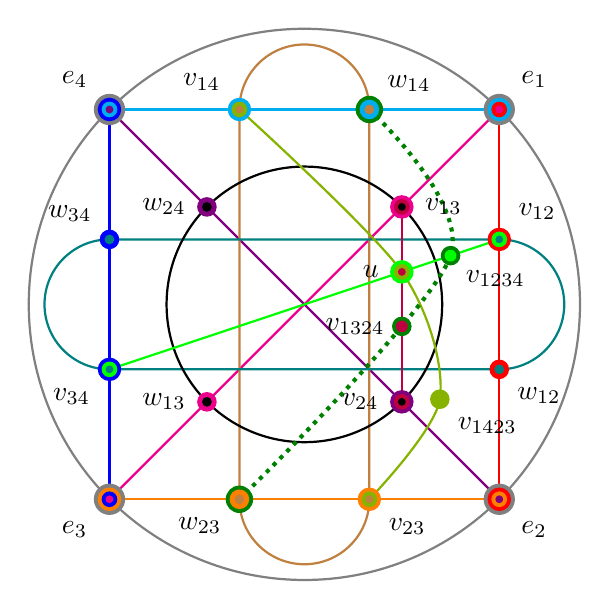
\begin{tikzpicture}[thick, scale=0.35]
    % --- Add necessary TikZ libraries ---
    \usetikzlibrary{decorations.markings, intersections}

    % --- 1. Define all colors ---
    \colorlet{colorCircle}{gray}
    \colorlet{colorE1E2}{red} \colorlet{colorE2E3}{orange}
    \colorlet{colorE3E4}{blue} \colorlet{colorE4E1}{cyan}
    \colorlet{colorV12V34}{green} \colorlet{colorV23V41}{lime!70!black}
    \colorlet{colorCurve13}{magenta} \colorlet{colorCurve24}{violet}
    \colorlet{colorV13V24}{purple}
    \colorlet{colorHiddenA}{brown} \colorlet{colorHiddenB}{teal}
    \colorlet{colorEllipse}{black}   %yellow!80!
    \colorlet{darkgreen}{green!50!black}

    % --- 2. Define geometric parameters ---
    \def\R{10} \def\bendangle{30}

    % --- 3. Define ALL coordinates first, without drawing ---
    \foreach \angle/\i in {45/1, 315/2, 225/3, 135/4} { \coordinate (e\i) at (\angle:\R); }
    \foreach \i/\j in {1/2, 2/3, 3/4, 4/1} {
        \coordinate (v\i\j) at ($(e\i)!1/3!(e\j)$);
        \coordinate (w\i\j) at ($(e\i)!2/3!(e\j)$);
    }
    \coordinate (v13) at ($(e1)!1/4!(e3)$);
    \coordinate (v24) at ($(e2)!1/4!(e4)$);
    \coordinate (w13) at ($(e1)!3/4!(e3)$);
    \coordinate (w24) at ($(e2)!3/4!(e4)$);

    % --- CHANGE: Define u at 0.6 of the distance along the curved green path from v34.
    % \path[
    %     postaction={decorate, decoration={
    %         markings,
    %         mark=at position 0.6 with {\coordinate (u) at (0,0);}
    %     }}
    % ] (v34) to[bend right=\bendangle/2] (v12);
    \path[name path=curve-v12-v34] (v34) -- (v12);
    \path[name path=curve-v13-v24] (v13) -- (v24);
    \path[name intersections={of=curve-v12-v34 and curve-v13-v24, by=u}];

    % All coordinates that depend on u will now be automatically updated.
    \coordinate (g12) at ($(u)!0.5!(v12)$);
    \coordinate (g13) at ($(u)!0.5!(v13)$);
    \coordinate (g23) at (325:\R*.6); % This is the coordinate for node v1423
    % \coordinate (g23) at ($(u)!0.8!(v41)$); % This is the coordinate for node v1423
    \path (e1) (v13) (w13) (e3);
    \path (e2) (v24) (w24) (e4);

    % --- 4. Draw all lines and curves ---
    \draw[colorCircle] (0,0) circle (\R);
    \draw[colorE1E2] (e1) -- (e2); \draw[colorE2E3] (e2) -- (e3);
    \draw[colorE3E4] (e3) -- (e4); \draw[colorE4E1] (e4) -- (e1);
    \draw[colorCurve13] (e1) -- (e3);
    \draw[colorCurve24] (e2) -- (e4);

    \draw[colorHiddenA] (v41) -- (w23); \draw[colorHiddenA] (w41) -- (v23);
    \draw[colorHiddenB] (v12) -- (w34); \draw[colorHiddenB] (w12) -- (v34);
    \draw[colorEllipse] (0,0) circle (\R/2);
    \draw[colorHiddenA] let \p1=($(w41)-(v41)$), \n1={atan2(\y1,\x1)}, \n2={veclen(\x1,\y1)/2} in (w41) arc (\n1:\n1+180:\n2);
    \draw[colorHiddenA] let \p1=($(w23)-(v23)$), \n1={atan2(\y1,\x1)}, \n2={veclen(\x1,\y1)/2} in (w23) arc (\n1:\n1+180:\n2);
    \draw[colorHiddenB] let \p1=($(w12)-(v12)$), \n1={atan2(\y1,\x1)}, \n2={veclen(\x1,\y1)/2} in (w12) arc (\n1:\n1+180:\n2);
    \draw[colorHiddenB] let \p1=($(w34)-(v34)$), \n1={atan2(\y1,\x1)}, \n2={veclen(\x1,\y1)/2} in (w34) arc (\n1:\n1+180:\n2);

    % Draw the green curve.
    % \draw[colorV12V34] (v34) to[bend right=\bendangle/2] (v12);
    \draw[colorV12V34] (v34) -- (v12);

    % The lime!70!black curve automatically adjusts to the new position of u.
    \draw[colorV23V41] plot[smooth, tension=0.5] coordinates {(v41) (u) (g23) (v23)};

    % Dotted green curve adjusts because its shape depends on g12, which depends on u.
    % \draw[darkgreen, dotted, line width=1.5pt,
    %     postaction={decorate, decoration={
    %         markings,
    %         mark=at position 0.15 with {\coordinate (v1324) at (0,0);}
    %     }}
    % ] plot[smooth cycle, tension=0.5] coordinates {(w41) (w23) (g12)};
    \draw[darkgreen, dotted, line width=1.5pt] plot[smooth, tension=0.5] coordinates {(w41) (g12) (w23)};
    \path[name path=curve-w41-w23] plot[smooth, tension=0.5] coordinates {(w41) (g12) (w23)};
    \path[name intersections={of=curve-w41-w23 and curve-v13-v24, by=v1324}];
    % The purple curve automatically adjusts to the new position of u.
    % \draw[colorV13V24] plot[smooth, tension=0.8] coordinates {(v24) %(v1324)
    % (u) (v13)};
    \draw[colorV13V24] (v24) -- (v13);
    % --- 5. Draw all points on TOP ---
    \node[circle, fill=darkgreen, inner sep=2.5pt] at (v1324) {};
    \node[circle, fill=colorV13V24, inner sep=1.5pt, label={left:$v_{1324}$}] at (v1324) {};

    \node[circle, fill=darkgreen, inner sep=2.5pt] at (g12) {};
    \node[circle, fill=colorV12V34, inner sep=1.5pt, label={below right:$v_{1234}$}] at (g12) {};
    \node[circle, fill=colorV23V41, inner sep=2.5pt, label={below right:$v_{1423}$}] at (g23) {};
    \node[circle, fill=colorV12V34, inner sep=3pt, label={left:$u$}] at (u) {}; \node[circle, fill=colorV23V41, inner sep=2pt] at (u) {}; \node[circle, fill=colorV13V24, inner sep=1pt] at (u) {};
    \node[circle, fill=colorCurve13, inner sep=3pt, label={right:$v_{13}$}] at (v13) {}; \node[circle, fill=colorV13V24, inner sep=2pt] at (v13) {}; \node[circle, fill=colorEllipse, inner sep=1pt] at (v13) {};
    \node[circle, fill=colorCurve24, inner sep=3pt, label={left:$v_{24}$}] at (v24) {}; \node[circle, fill=colorV13V24, inner sep=2pt] at (v24) {}; \node[circle, fill=colorEllipse, inner sep=1pt] at (v24) {};
    \node[circle, fill=colorCurve13, inner sep=2.5pt, label={left:$w_{13}$}] at (w13) {}; \node[circle, fill=colorEllipse, inner sep=1.25pt] at (w13) {};
    \node[circle, fill=colorCurve24, inner sep=2.5pt, label={left:$w_{24}$}] at (w24) {}; \node[circle, fill=colorEllipse, inner sep=1.25pt] at (w24) {};
    \node[circle, fill=darkgreen, inner sep=3.5pt] at (w41) {};
    \node[circle, fill=colorE4E1, inner sep=2.5pt, label={above right:$w_{14}$}] at (w41) {}; \node[circle, fill=colorHiddenA, inner sep=1.25pt] at (w41) {};
    \node[circle, fill=darkgreen, inner sep=3.5pt] at (w23) {};
    \node[circle, fill=colorE2E3, inner sep=2.5pt, label={below left:$w_{23}$}] at (w23) {}; \node[circle, fill=colorHiddenA, inner sep=1.25pt] at (w23) {};
    \node[circle, fill=colorE4E1, inner sep=3pt, label={above left:$v_{14}$}] at (v41) {}; \node[circle, fill=colorV23V41, inner sep=2pt] at (v41) {}; \node[circle, fill=colorHiddenA, inner sep=1pt] at (v41) {};
    \node[circle, fill=colorE2E3, inner sep=3pt, label={below right:$v_{23}$}] at (v23) {}; \node[circle, fill=colorV23V41, inner sep=2pt] at (v23) {}; \node[circle, fill=colorHiddenA, inner sep=1pt] at (v23) {};
    \node[circle, fill=colorE1E2, inner sep=3pt, label={above right:$v_{12}$}] at (v12) {}; \node[circle, fill=colorV12V34, inner sep=2pt] at (v12) {}; \node[circle, fill=colorHiddenB, inner sep=1pt] at (v12) {};
    \node[circle, fill=colorE1E2, inner sep=2.5pt, label={below right:$w_{12}$}] at (w12) {}; \node[circle, fill=colorHiddenB, inner sep=1.25pt] at (w12) {};
    \node[circle, fill=colorE3E4, inner sep=3pt, label={below left:$v_{34}$}] at (v34) {}; \node[circle, fill=colorV12V34, inner sep=2pt] at (v34) {}; \node[circle, fill=colorHiddenB, inner sep=1pt] at (v34) {};
    \node[circle, fill=colorE3E4, inner sep=2.5pt, label={above left:$w_{34}$}] at (w34) {}; \node[circle, fill=colorHiddenB, inner sep=1.25pt] at (w34) {};
    \node[circle, fill=colorCircle, inner sep=4pt, label={45:$e_1$}] at (e1) {}; \node[circle, fill=colorE4E1, inner sep=3pt] at (e1) {}; \node[circle, fill=colorE1E2, inner sep=2pt] at (e1) {}; \node[circle, fill=colorCurve13, inner sep=1pt] at (e1) {};
    \node[circle, fill=colorCircle, inner sep=4pt, label={315:$e_2$}] at (e2) {}; \node[circle, fill=colorE1E2, inner sep=3pt] at (e2) {}; \node[circle, fill=colorE2E3, inner sep=2pt] at (e2) {}; \node[circle, fill=colorCurve24, inner sep=1pt] at (e2) {};
    \node[circle, fill=colorCircle, inner sep=4pt, label={225:$e_3$}] at (e3) {}; \node[circle, fill=colorE2E3, inner sep=3pt] at (e3) {}; \node[circle, fill=colorE3E4, inner sep=2pt] at (e3) {}; \node[circle, fill=colorCurve13, inner sep=1pt] at (e3) {};
    \node[circle, fill=colorCircle, inner sep=4pt, label={135:$e_4$}] at (e4) {}; \node[circle, fill=colorE3E4, inner sep=3pt] at (e4) {}; \node[circle, fill=colorE4E1, inner sep=2pt] at (e4) {}; \node[circle, fill=colorCurve24, inner sep=1pt] at (e4) {};

\end{tikzpicture}
&\qquad \qquad \qquad &
%\resizebox{0.4\textwidth}{!}{
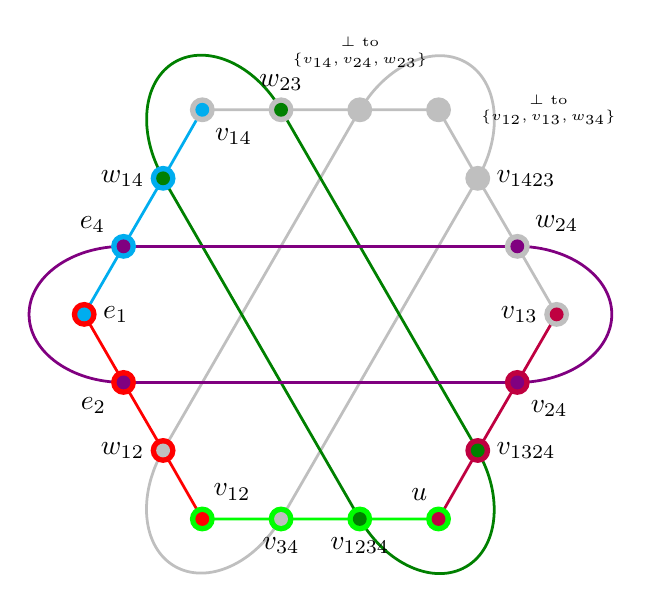
\begin{tikzpicture}  [ultra thick, scale=0.6]

    % --- 1. Define all colors ---
    \colorlet{colorE1E2}{red} \colorlet{colorE4E1}{cyan}
    \colorlet{colorV12V34}{green} \colorlet{colorV13V24}{purple}
    \colorlet{colorCurve24}{violet} \colorlet{lightgray}{gray!50!}
    \colorlet{darkgreen}{green!50!black}

    % --- 2. Define TikZ styles ---
    \tikzstyle{every path}=[line width=1pt]
    \tikzstyle{c2}=[circle,inner sep=3pt,minimum size=9pt]
    \tikzstyle{c1}=[circle,inner sep=0pt,minimum size=5pt]

    % --- 3. Define positions ---
    \path
              (240:5) coordinate(1) (-0.833,-4.33) coordinate(2)
              (0.833,-4.33) coordinate(3) (300:5) coordinate(4)
              (3.33,-2.88) coordinate(5) (4.167,-1.44) coordinate(6)
              (0:5) coordinate(7) (4.167,1.44) coordinate(8)
              (3.33,2.88) coordinate(9) (60:5) coordinate(10)
              (0.833,4.33) coordinate(11) (-0.833,4.33) coordinate(12)
              (120:5) coordinate(13) (-3.33,2.88) coordinate(14)
              (-4.167,1.44) coordinate(15) (180:5) coordinate(16)
              (-4.167,-1.44) coordinate(17) (-3.33,-2.88) coordinate(18);

    % --- 4. Draw context curves ---
    \draw [color=lightgray] (7) -- (8) -- (9)-- (10);
    \draw [color=lightgray] (10) -- (11) -- (12) -- (13);
    \draw [color=lightgray] (9) -- (2); \draw [color=lightgray] (11) -- (18);
    \draw [rotate=240,color=lightgray] (9) arc (90:270:2 and 1.44); \draw[rotate=60,color=lightgray] (18) arc (90:270:2 and 1.44);
    \draw [color=darkgreen] (12) -- (5); \draw [color=darkgreen] (14) -- (3);
    \draw[rotate=300,color=darkgreen] (12) arc (90:270:2 and 1.44); \draw[rotate=120,color=darkgreen] (3) arc (90:270:2 and 1.44);
    \draw [color=colorE4E1] (13) -- (14) -- (15) -- (16);
    \draw [color=colorE1E2] (16) -- (17) -- (18) -- (1);
    \draw [color=colorV12V34] (1) -- (2) -- (3) -- (4);
    \draw [color=colorV13V24] (4) -- (5) -- (6) -- (7);
    \draw [color=colorCurve24] (8) -- (15); \draw [color=colorCurve24](17) -- (6);
    \draw [color=colorCurve24] (8) arc (450:270:2 and 1.44); \draw [color=colorCurve24] (15) arc (90:270:2 and 1.44);

    % --- 5. Draw observables with corrected labels ---
    \draw (1) coordinate[c2,fill=colorV12V34]; \draw (1) coordinate[c1,fill=colorE1E2,label=85:$v_{12}$];
    \draw (2) coordinate[c2,fill=colorV12V34]; \draw (2) coordinate[c1,fill=lightgray,label=270:$v_{34}$];
    \draw (3) coordinate[c2,fill=colorV12V34]; \draw (3) coordinate[c1,fill=darkgreen,label=270:$v_{1234}$];
    \draw (4) coordinate[c2,fill=colorV12V34]; \draw (4) coordinate[c1,fill=colorV13V24,label=95:$u$];
    \draw (5) coordinate[c2,fill=colorV13V24]; \draw (5) coordinate[c1,fill=darkgreen,label=0:$v_{1324}$];
    \draw (6) coordinate[c2,fill=colorV13V24]; \draw (6) coordinate[c1,fill=colorCurve24,label=290:$v_{24}$];
    \draw (7) coordinate[c2,fill=lightgray]; \draw (7) coordinate[c1,fill=colorV13V24,label=180:$v_{13}$];
    \draw (8) coordinate[c2,fill=lightgray]; \draw (8) coordinate[c1,fill=colorCurve24,label=30:$w_{24}$];
    \draw (9) coordinate[c2,fill=lightgray]; \draw (9) coordinate[c1,fill=lightgray,label=0:$v_{1423}$];
    % --- MODIFIED: Explicit construction labels ---
    \draw (10) coordinate[c2,fill=lightgray]; \draw (10) coordinate[c1,fill=lightgray,label={[label distance=3mm,align=center, font=\tiny]0:$\perp$ to \\ $\{v_{12}, v_{13}, w_{34}\}$ }];
    \draw (11) coordinate[c2,fill=lightgray]; \draw (11) coordinate[c1,fill=lightgray,label={[label distance=3mm,align=center, font=\tiny]90:$\perp$ to \\ $\{v_{14}, v_{24}, w_{23}\}$ }];
    \draw (12) coordinate[c2,fill=lightgray]; \draw (12) coordinate[c1,fill=darkgreen,label=90:$w_{23}$];
    \draw (13) coordinate[c2,fill=lightgray]; \draw (13) coordinate[c1,fill=colorE4E1,label=285:$v_{14}$];
    \draw (14) coordinate[c2,fill=colorE4E1]; \draw (14) coordinate[c1,fill=darkgreen,label=180:$w_{14}$];
    \draw (15) coordinate[c2,fill=colorE4E1]; \draw (15) coordinate[c1,fill=colorCurve24,label=160:$e_4$];
    \draw (16) coordinate[c2,fill=colorE1E2]; \draw (16) coordinate[c1,fill=colorE4E1,label=0:$e_1$];
    \draw (17) coordinate[c2,fill=colorE1E2]; \draw (17) coordinate[c1,fill=colorCurve24,label=215:$e_2$];
    \draw (18) coordinate[c2,fill=colorE1E2]; \draw (18) coordinate[c1,fill=lightgray,label=180:$w_{12}$];

\end{tikzpicture}
%}
\\
(a)&&(b)
% \\
% \begin{tikzpicture}[ultra thick, scale=0.35]

%     % --- 1. Define all colors ---
%     \colorlet{colorCircle}{gray}
%     \colorlet{colorE1E2}{red} \colorlet{colorE2E3}{orange}
%     \colorlet{colorE3E4}{blue} \colorlet{colorE4E1}{cyan}
%     \colorlet{colorV12V34}{green} \colorlet{colorV23V41}{lime!70!black}
%     \colorlet{colorCurve13}{magenta} \colorlet{colorCurve24}{violet}
%     \colorlet{colorV13V24}{purple}
%     \colorlet{colorHiddenA}{brown} \colorlet{colorHiddenB}{teal}
%     \colorlet{colorEllipse}{black}   %yellow!80!
%     \colorlet{darkgreen}{green!50!black}

%     % --- 2. Define geometric parameters ---
%     \def\R{10} \def\bendangle{30}

%     % --- 3. Define ALL coordinates first, without drawing ---
% %    \coordinate (u) at (\R/5,0);
%     \foreach \angle/\i in {45/1, 315/2, 225/3, 135/4} { \coordinate (e\i) at (\angle:\R); }
%     \foreach \i/\j in {1/2, 2/3, 3/4, 4/1} {
%         \coordinate (v\i\j) at ($(e\i)!1/3!(e\j)$);
%         \coordinate (w\i\j) at ($(e\i)!2/3!(e\j)$);
%     }
%     \coordinate (v13) at ($(e1)!1/4!(e3)$);
%     \coordinate (v24) at ($(e2)!1/4!(e4)$);
%     \coordinate (w13) at ($(e1)!3/4!(e3)$);
%     \coordinate (w24) at ($(e2)!3/4!(e4)$);
%     \def\vlineangle{63.43}
%     \path[name path=alignment-line] (\vlineangle:\R) -- (\vlineangle+180:\R);
% %    \path[name path=curve-e1-e3] (e1) to[bend right=\bendangle] (e3);
% %    \path[name path=curve-e2-e4] (v23) to[bend right] (v41);
%     \path[name path=curve-v12-v34] (v34) to[bend right] (v12);
%     \path[name path=curve-v23-v14] (v23) to[bend right] (v41);
%     \path[name intersections={of=curve-v12-v34 and curve-v23-v14, by=u}];
% %    \path[name intersections={of=alignment-line and curve-e1-e3, by=v13}];
% %    \path[name intersections={of=alignment-line and curve-e2-e4, by=v24}];
%     \coordinate (g12) at ($(u)!0.5!(v12)$);
%     \coordinate (g13) at ($(u)!0.5!(v13)$);
%     \coordinate (g23) at ($(u)!0.5!(v23)$);
%     \path (e1) (v13)%to[bend right=\bendangle] coordinate[pos=0.85]
%     (w13) (e3);
%     \path (e2) (v24)%to[bend left=\bendangle] coordinate[pos=0.75]
%     (w24) (e4);

%     % --- 4. Draw all lines and curves ---
%     \draw[colorCircle] (0,0) circle (\R);
%     \draw[colorE1E2] (e1) -- (e2); \draw[colorE2E3] (e2) -- (e3);
%     \draw[colorE3E4] (e3) -- (e4); \draw[colorE4E1] (e4) -- (e1);
% %    \draw[colorV12V34] (v12) -- (v34); \draw[colorV23V41] (v23) -- (v41);
%     \draw[colorCurve13] (e1) -- %to[bend right=\bendangle]
%     (e3);
%     \draw[colorCurve24] (e2) -- %to[bend left=\bendangle]
%     (e4);
%     \draw[colorV13V24] (v13) -- (v24);
%     \draw[colorHiddenA] (v41) -- (w23); \draw[colorHiddenA] (w41) -- (v23);
%     \draw[colorHiddenB] (v12) -- (w34); \draw[colorHiddenB] (w12) -- (v34);
%     \draw[colorEllipse] (0,0) circle (\R/2);
% %    \draw[colorEllipse] plot[smooth cycle, tension=0.8] coordinates {(v13) (w24) (w13) (v24)};
%     \draw[colorHiddenA] let \p1=($(w41)-(v41)$), \n1={atan2(\y1,\x1)}, \n2={veclen(\x1,\y1)/2} in (w41) arc (\n1:\n1+180:\n2);
%     \draw[colorHiddenA] let \p1=($(w23)-(v23)$), \n1={atan2(\y1,\x1)}, \n2={veclen(\x1,\y1)/2} in (w23) arc (\n1:\n1+180:\n2);
%     \draw[colorHiddenB] let \p1=($(w12)-(v12)$), \n1={atan2(\y1,\x1)}, \n2={veclen(\x1,\y1)/2} in (w12) arc (\n1:\n1+180:\n2);
%     \draw[colorHiddenB] let \p1=($(w34)-(v34)$), \n1={atan2(\y1,\x1)}, \n2={veclen(\x1,\y1)/2} in (w34) arc (\n1:\n1+180:\n2);

%     \draw[colorV12V34] (v34) to[bend right=\bendangle/3] (v12);
%     \draw[colorV12V34] (v23) to[bend right] (v41);

%     % --- MODIFIED: Emergent block shown with a DOTTED dark green curve ---
%     \draw[darkgreen, dotted, line width=1.5pt] plot[smooth cycle, tension=0.8] coordinates {(w41) %(g13)
%     (w23) (g12)
%     };

%     % --- 5. Draw all points on TOP ---
%     \node[circle, fill=darkgreen, inner sep=2.5pt] at (g13) {};
%     \node[circle, fill=colorV13V24, inner sep=1.5pt, label={left:$v_{1324}$}] at (g13) {};
%     \node[circle, fill=darkgreen, inner sep=2.5pt] at (g12) {};
%     \node[circle, fill=colorV12V34, inner sep=1.5pt, label={below:$v_{1234}$}] at (g12) {};
%     \node[circle, fill=colorV23V41, inner sep=1.5pt, label={above left:$v_{1423}$}] at (g23) {};
%     \node[circle, fill=colorV12V34, inner sep=3pt, label={above left:$u$}] at (u) {}; \node[circle, fill=colorV23V41, inner sep=2pt] at (u) {}; \node[circle, fill=colorV13V24, inner sep=1pt] at (u) {};
% %    \node[circle, fill=colorV12V34, inner sep=3pt, label={above left:$u$}] at (u) {}; \node[circle, fill=colorV23V41, inner sep=2pt] at (u) {}; \node[circle, fill=colorV13V24, inner sep=1pt] at (u) {};
%     \node[circle, fill=colorCurve13, inner sep=3pt, label={above:$v_{13}$}] at (v13) {}; \node[circle, fill=colorV13V24, inner sep=2pt] at (v13) {}; \node[circle, fill=colorEllipse, inner sep=1pt] at (v13) {};
%     \node[circle, fill=colorCurve24, inner sep=3pt, label={below:$v_{24}$}] at (v24) {}; \node[circle, fill=colorV13V24, inner sep=2pt] at (v24) {}; \node[circle, fill=colorEllipse, inner sep=1pt] at (v24) {};
%     \node[circle, fill=colorCurve13, inner sep=2.5pt, label={right:$w_{13}$}] at (w13) {}; \node[circle, fill=colorEllipse, inner sep=1.25pt] at (w13) {};
%     \node[circle, fill=colorCurve24, inner sep=2.5pt, label={below left:$w_{24}$}] at (w24) {}; \node[circle, fill=colorEllipse, inner sep=1.25pt] at (w24) {};
%     \node[circle, fill=darkgreen, inner sep=3.5pt] at (w41) {};
%     \node[circle, fill=colorE4E1, inner sep=2.5pt, label={above right:$w_{14}$}] at (w41) {}; \node[circle, fill=colorHiddenA, inner sep=1.25pt] at (w41) {};
%     \node[circle, fill=darkgreen, inner sep=3.5pt] at (w23) {};
%     \node[circle, fill=colorE2E3, inner sep=2.5pt, label={below left:$w_{23}$}] at (w23) {}; \node[circle, fill=colorHiddenA, inner sep=1.25pt] at (w23) {};
%     \node[circle, fill=colorE4E1, inner sep=3pt, label={above left:$v_{14}$}] at (v41) {}; \node[circle, fill=colorV23V41, inner sep=2pt] at (v41) {}; \node[circle, fill=colorHiddenA, inner sep=1pt] at (v41) {};
%     \node[circle, fill=colorE2E3, inner sep=3pt, label={below right:$v_{23}$}] at (v23) {}; \node[circle, fill=colorV23V41, inner sep=2pt] at (v23) {}; \node[circle, fill=colorHiddenA, inner sep=1pt] at (v23) {};
%     \node[circle, fill=colorE1E2, inner sep=3pt, label={above right:$v_{12}$}] at (v12) {}; \node[circle, fill=colorV12V34, inner sep=2pt] at (v12) {}; \node[circle, fill=colorHiddenB, inner sep=1pt] at (v12) {};
%     \node[circle, fill=colorE1E2, inner sep=2.5pt, label={below right:$w_{12}$}] at (w12) {}; \node[circle, fill=colorHiddenB, inner sep=1.25pt] at (w12) {};
%     \node[circle, fill=colorE3E4, inner sep=3pt, label={below left:$v_{34}$}] at (v34) {}; \node[circle, fill=colorV12V34, inner sep=2pt] at (v34) {}; \node[circle, fill=colorHiddenB, inner sep=1pt] at (v34) {};
%     \node[circle, fill=colorE3E4, inner sep=2.5pt, label={above left:$w_{34}$}] at (w34) {}; \node[circle, fill=colorHiddenB, inner sep=1.25pt] at (w34) {};
%     \node[circle, fill=colorCircle, inner sep=4pt, label={45:$e_1$}] at (e1) {}; \node[circle, fill=colorE4E1, inner sep=3pt] at (e1) {}; \node[circle, fill=colorE1E2, inner sep=2pt] at (e1) {}; \node[circle, fill=colorCurve13, inner sep=1pt] at (e1) {};
%     \node[circle, fill=colorCircle, inner sep=4pt, label={315:$e_2$}] at (e2) {}; \node[circle, fill=colorE1E2, inner sep=3pt] at (e2) {}; \node[circle, fill=colorE2E3, inner sep=2pt] at (e2) {}; \node[circle, fill=colorCurve24, inner sep=1pt] at (e2) {};
%     \node[circle, fill=colorCircle, inner sep=4pt, label={225:$e_3$}] at (e3) {}; \node[circle, fill=colorE2E3, inner sep=3pt] at (e3) {}; \node[circle, fill=colorE3E4, inner sep=2pt] at (e3) {}; \node[circle, fill=colorCurve13, inner sep=1pt] at (e3) {};
%     \node[circle, fill=colorCircle, inner sep=4pt, label={135:$e_4$}] at (e4) {}; \node[circle, fill=colorE3E4, inner sep=3pt] at (e4) {}; \node[circle, fill=colorE4E1, inner sep=2pt] at (e4) {}; \node[circle, fill=colorCurve24, inner sep=1pt] at (e4) {};

% \end{tikzpicture}
% &&
% %\resizebox{0.4\textwidth}{!}{
% \begin{tikzpicture}[thick, scale=0.35]

%     % --- 1. Define all colors ---
%     \colorlet{colorCircle}{gray}
%     \colorlet{colorE1E2}{red} \colorlet{colorE2E3}{orange}
%     \colorlet{colorE3E4}{blue} \colorlet{colorE4E1}{cyan}
%     \colorlet{colorV12V34}{green} \colorlet{colorV23V41}{lime!70!black}
%     \colorlet{colorCurve13}{magenta} \colorlet{colorCurve24}{violet}
%     \colorlet{colorV13V24}{purple}
%     \colorlet{colorHiddenA}{brown} \colorlet{colorHiddenB}{teal}
%     \colorlet{colorEllipse}{black}   %yellow!80!
%     \colorlet{darkgreen}{green!50!black}

%     % --- 2. Define geometric parameters ---
%     \def\R{10} \def\bendangle{30}

%     % --- 3. Define ALL coordinates first, without drawing ---
%     \coordinate (u) at (0,0);
%     \foreach \angle/\i in {45/1, 315/2, 225/3, 135/4} { \coordinate (e\i) at (\angle:\R); }
%     \foreach \i/\j in {1/2, 2/3, 3/4, 4/1} {
%         \coordinate (v\i\j) at ($(e\i)!1/3!(e\j)$);
%         \coordinate (w\i\j) at ($(e\i)!2/3!(e\j)$);
%     }
%     \def\vlineangle{63.43}
%     \path[name path=alignment-line] (\vlineangle:\R) -- (\vlineangle+180:\R);
%     \path[name path=curve-e1-e3] (e1) to[bend right=\bendangle] (e3);
%     \path[name path=curve-e2-e4] (e2) to[bend left=\bendangle] (e4);
%     \path[name intersections={of=alignment-line and curve-e1-e3, by=v13}];
%     \path[name intersections={of=alignment-line and curve-e2-e4, by=v24}];
%     \coordinate (g13) at ($(u)!0.5!(v13)$); \coordinate (g12) at ($(u)!0.5!(v12)$);
%     \coordinate (g23) at ($(u)!0.5!(v23)$);
%     \path (e1) to[bend right=\bendangle] coordinate[pos=0.85] (w13) (e3);
%     \path (e2) to[bend left=\bendangle] coordinate[pos=0.75] (w24) (e4);

%     % --- 4. Draw all lines and curves ---
%     \draw[colorCircle] (0,0) circle (\R);
%     \draw[colorE1E2] (e1) -- (e2); \draw[colorE2E3] (e2) -- (e3);
%     \draw[colorE3E4] (e3) -- (e4); \draw[colorE4E1] (e4) -- (e1);
%     \draw[colorV12V34] (v12) -- (v34); \draw[colorV23V41] (v23) -- (v41);
%     \draw[colorCurve13] (e1) to[bend right=\bendangle] (e3);
%     \draw[colorCurve24] (e2) to[bend left=\bendangle] (e4);
%     \draw[colorV13V24] (v13) -- (v24);
%     \draw[colorHiddenA] (v41) -- (w23); \draw[colorHiddenA] (w41) -- (v23);
%     \draw[colorHiddenB] (v12) -- (w34); \draw[colorHiddenB] (w12) -- (v34);
%     \draw[colorEllipse] plot[smooth cycle, tension=0.8] coordinates {(v13) (w24) (w13) (v24)};
%     \draw[colorHiddenA] let \p1=($(w41)-(v41)$), \n1={atan2(\y1,\x1)}, \n2={veclen(\x1,\y1)/2} in (w41) arc (\n1:\n1+180:\n2);
%     \draw[colorHiddenA] let \p1=($(w23)-(v23)$), \n1={atan2(\y1,\x1)}, \n2={veclen(\x1,\y1)/2} in (w23) arc (\n1:\n1+180:\n2);
%     \draw[colorHiddenB] let \p1=($(w12)-(v12)$), \n1={atan2(\y1,\x1)}, \n2={veclen(\x1,\y1)/2} in (w12) arc (\n1:\n1+180:\n2);
%     \draw[colorHiddenB] let \p1=($(w34)-(v34)$), \n1={atan2(\y1,\x1)}, \n2={veclen(\x1,\y1)/2} in (w34) arc (\n1:\n1+180:\n2);

%     % --- MODIFIED: Emergent block shown with a DOTTED dark green curve ---
%     \draw[darkgreen, dotted, line width=1.5pt] plot[smooth cycle, tension=0.8] coordinates {(w41) (g13) (w23) (g12)};

%     % --- 5. Draw all points on TOP ---
%     \node[circle, fill=darkgreen, inner sep=2.5pt] at (g13) {};
%     \node[circle, fill=colorV13V24, inner sep=1.5pt, label={left:$v_{1324}$}] at (g13) {};
%     \node[circle, fill=darkgreen, inner sep=2.5pt] at (g12) {};
%     \node[circle, fill=colorV12V34, inner sep=1.5pt, label={below:$v_{1234}$}] at (g12) {};
%     \node[circle, fill=colorV23V41, inner sep=1.5pt, label={above left:$v_{1423}$}] at (g23) {};
%     \node[circle, fill=colorV12V34, inner sep=3pt, label={above left:$u$}] at (u) {}; \node[circle, fill=colorV23V41, inner sep=2pt] at (u) {}; \node[circle, fill=colorV13V24, inner sep=1pt] at (u) {};
%     \node[circle, fill=colorCurve13, inner sep=3pt, label={above:$v_{13}$}] at (v13) {}; \node[circle, fill=colorV13V24, inner sep=2pt] at (v13) {}; \node[circle, fill=colorEllipse, inner sep=1pt] at (v13) {};
%     \node[circle, fill=colorCurve24, inner sep=3pt, label={below:$v_{24}$}] at (v24) {}; \node[circle, fill=colorV13V24, inner sep=2pt] at (v24) {}; \node[circle, fill=colorEllipse, inner sep=1pt] at (v24) {};
%     \node[circle, fill=colorCurve13, inner sep=2.5pt, label={right:$w_{13}$}] at (w13) {}; \node[circle, fill=colorEllipse, inner sep=1.25pt] at (w13) {};
%     \node[circle, fill=colorCurve24, inner sep=2.5pt, label={below left:$w_{24}$}] at (w24) {}; \node[circle, fill=colorEllipse, inner sep=1.25pt] at (w24) {};
%     \node[circle, fill=darkgreen, inner sep=3.5pt] at (w41) {};
%     \node[circle, fill=colorE4E1, inner sep=2.5pt, label={above right:$w_{14}$}] at (w41) {}; \node[circle, fill=colorHiddenA, inner sep=1.25pt] at (w41) {};
%     \node[circle, fill=darkgreen, inner sep=3.5pt] at (w23) {};
%     \node[circle, fill=colorE2E3, inner sep=2.5pt, label={below left:$w_{23}$}] at (w23) {}; \node[circle, fill=colorHiddenA, inner sep=1.25pt] at (w23) {};
%     \node[circle, fill=colorE4E1, inner sep=3pt, label={above left:$v_{14}$}] at (v41) {}; \node[circle, fill=colorV23V41, inner sep=2pt] at (v41) {}; \node[circle, fill=colorHiddenA, inner sep=1pt] at (v41) {};
%     \node[circle, fill=colorE2E3, inner sep=3pt, label={below right:$v_{23}$}] at (v23) {}; \node[circle, fill=colorV23V41, inner sep=2pt] at (v23) {}; \node[circle, fill=colorHiddenA, inner sep=1pt] at (v23) {};
%     \node[circle, fill=colorE1E2, inner sep=3pt, label={above right:$v_{12}$}] at (v12) {}; \node[circle, fill=colorV12V34, inner sep=2pt] at (v12) {}; \node[circle, fill=colorHiddenB, inner sep=1pt] at (v12) {};
%     \node[circle, fill=colorE1E2, inner sep=2.5pt, label={below right:$w_{12}$}] at (w12) {}; \node[circle, fill=colorHiddenB, inner sep=1.25pt] at (w12) {};
%     \node[circle, fill=colorE3E4, inner sep=3pt, label={below left:$v_{34}$}] at (v34) {}; \node[circle, fill=colorV12V34, inner sep=2pt] at (v34) {}; \node[circle, fill=colorHiddenB, inner sep=1pt] at (v34) {};
%     \node[circle, fill=colorE3E4, inner sep=2.5pt, label={above left:$w_{34}$}] at (w34) {}; \node[circle, fill=colorHiddenB, inner sep=1.25pt] at (w34) {};
%     \node[circle, fill=colorCircle, inner sep=4pt, label={45:$e_1$}] at (e1) {}; \node[circle, fill=colorE4E1, inner sep=3pt] at (e1) {}; \node[circle, fill=colorE1E2, inner sep=2pt] at (e1) {}; \node[circle, fill=colorCurve13, inner sep=1pt] at (e1) {};
%     \node[circle, fill=colorCircle, inner sep=4pt, label={315:$e_2$}] at (e2) {}; \node[circle, fill=colorE1E2, inner sep=3pt] at (e2) {}; \node[circle, fill=colorE2E3, inner sep=2pt] at (e2) {}; \node[circle, fill=colorCurve24, inner sep=1pt] at (e2) {};
%     \node[circle, fill=colorCircle, inner sep=4pt, label={225:$e_3$}] at (e3) {}; \node[circle, fill=colorE2E3, inner sep=3pt] at (e3) {}; \node[circle, fill=colorE3E4, inner sep=2pt] at (e3) {}; \node[circle, fill=colorCurve13, inner sep=1pt] at (e3) {};
%     \node[circle, fill=colorCircle, inner sep=4pt, label={135:$e_4$}] at (e4) {}; \node[circle, fill=colorE3E4, inner sep=3pt] at (e4) {}; \node[circle, fill=colorE4E1, inner sep=2pt] at (e4) {}; \node[circle, fill=colorCurve24, inner sep=1pt] at (e4) {};

% \end{tikzpicture}
% %}
\end{tabular}
\caption{
(a)
Generalization of the Harding and Salinas Schmeis 3-uniform hypergraph scheme~\cite{harding2025remarksIJTP} in 4 dimensions.
Solid curves represent structurally imposed orthogonal bases (contexts),
while the \textit{dotted dark green curve} highlights an additional  emergent  basis,
$\{w_{14}, w_{23}, v_{1234}, v_{1324}\}$. Its orthogonality is not imposed by construction
but arises as a consequence of the gadget forcing the center vector $u$
into a state of maximal unbiasedness (like a vector from a MUB relative to the computational basis).
(b)
The Kochen--Specker configuration of Cabello et al.~\cite{cabello-96} (labels from Cabello~\cite{cabello:210401})
relabeled with the vector notation from the gadget construction.
 This labeling highlights the informational equivalence of the two vector sets,
ignoring overall signs for simplicity as they represent the same one-dimensional subspaces.
\\
Notice that this Greechie diagram contains loops of order 4 and couples of edges intersecting in two vertices. This is allowed in orthomodular lattices only under special conditions which are difficult to verify in the diagram itself~\cite{kalmbach-83}.
Thus previous works tried to avoid this situation and did not consider such Greechie diagrams.
(However, our diagram is still not complete; some blocks are not drawn.)
Here we know the vector representation which guarantees the correctness of the diagram.
This might found applications also in the mathematical studies of orthomodular lattices, which lack such examples.
}
\label{fig:peres}
\end{figure*}




\begin{table*}[ht]
\caption{Comprehensive comparison and informational equivalence of the 20-vector Gadget Set
and the 18-vector set by Cabello et al.~\cite{cabello-96,cabello:210401}.
Both sets are shown to be subsets of the 24-vector
Peres set~\cite{peres111,mermin90b,peres-91}
which represents the complete eigensystem of the Peres--Mermin square~\cite{pavicic-2004ksafq,svozil-2024-convert-pra-externalfigures}.
Vectors unique to one of the smaller sets are shown to be uniquely constructible from the other,
demonstrating their underlying geometric equivalence.
The labels $v_{ij}$ in this column correspond to the 18-vector diagram~\cite{cabello-96}
(labels from Cabello~\cite{cabello:210401}).}
\label{tab:vector-equivalence}
\begin{ruledtabular}
\begin{tabular}{cccc}
Gadget Label & Gadget Vector & Cabello Diagram Label & Vector Construction / Definition \\
\hline
$u$ & $(1,1,1,1)$ & $v_{56}$ & $(1,1,1,1)$ \\
$e_1$ & $(1,0,0,0)$ & $v_{12}$ & $(1,0,0,0)$ \\
$e_2$ & $(0,1,0,0)$ & $v_{18}$ & $(0,1,0,0)$ \\
$e_3$ & $(0,0,1,0)$ & (Constructed) & $\perp \text{ to } \{v_{12}, v_{18}, v_{28}\}$ \\
$e_4$ & $(0,0,0,1)$ & $v_{28}$ & $(0,0,0,1)$ \\
\hline
$v_{12}$ & $(0,0,1,-1)$ & $v_{16}$ & $(0,0,1,-1)$ \\
$v_{13}$ & $(0,-1,0,1)$ & $v_{45}$ & $(0,1,0,-1)$ \\
$v_{14}$ & $(0,1,-1,0)$ & $v_{23}$ & $(0,1,-1,0)$ \\
$v_{23}$ & $(1,0,0,-1)$ & (Constructed) & $\perp \text{ to } \{v_{18}, v_{23}, v_{29}\}$ \\
$v_{24}$ & $(-1,0,1,0)$ & $v_{58}$ & $(1,0,-1,0)$ \\
$v_{34}$ & $(1,-1,0,0)$ & $v_{67}$ & $(1,-1,0,0)$ \\
\hline
$w_{12}$ & $(0,0,1,1)$ & $v_{17}$ & $(0,0,1,1)$ \\
$w_{13}$ & $(0,1,0,1)$ & (Constructed) & $\perp \text{ to } \{v_{12}, v_{23}, v_{58}\}$ \\
$w_{14}$ & $(0,1,1,0)$ & $v_{29}$ & $(0,1,1,0)$ \\
$w_{23}$ & $(1,0,0,1)$ & $v_{39}$ & $(1,0,0,1)$ \\
$w_{24}$ & $(1,0,1,0)$ & $v_{48}$ & $(1,0,1,0)$ \\
$w_{34}$ & $(1,1,0,0)$ & (Constructed) & $\perp \text{ to } \{v_{16}, v_{17}, v_{28}\}$ \\
\hline
$v_{1234}$ & $(1,1,-1,-1)$ & $v_{69}$ & $(1,1,-1,-1)$ \\
$v_{1324}$ & $(1,-1,1,-1)$ & $v_{59}$ & $(1,-1,1,-1)$ \\
$v_{1423}$ & $(1,-1,-1,1)$ & $v_{47}$ & $(1,1,-1,1)$ \\
\hline
(Constructed) & $\perp \text{ to } \{v_{12}, v_{13}, w_{34}\}$ & $v_{34}$ & $(-1,1,1,1)$ \\
(Constructed) & $\perp \text{ to } \{v_{14}, v_{24}, w_{23}\}$ & $v_{37}$ & $(1,1,1,-1)$ \\
\end{tabular}
\end{ruledtabular}
\end{table*}





\subsubsection{Concrete $D=4$ example: $u=(1,1,1,1)$}

Take the center vector $u=(1,1,1,1)$ and the rim vectors
\begin{align*}
e_1&=(1,0,0,0),& e_2 =(0,1,0,0),\\
e_3&=(0,0,1,0),& e_4 =(0,0,0,1).
\end{align*}
The pair minors and their complementary vectors become:
\begin{align*}
v_{12}&=(0,0,1,-1), & w_{12}&=(0,0,1,1),\\
v_{13}&=(0,-1,0,1), & w_{13}&=(0,1,0,1),\\
v_{14}&=(0,1,-1,0), & w_{14}&=(0,1,1,0),\\
v_{23}&=(1,0,0,-1), & w_{23}&=(1,0,0,1),\\
v_{24}&=(-1,0,1,0), & w_{24}&=(1,0,1,0),\\
v_{34}&=(1,-1,0,0), & w_{34}&=(1,1,0,0).
\end{align*}
Each pair block
\[
\mathcal{B}_{ij}=\{e_i, e_j, v_{ij}, w_{ij}\}
\]
forms an ONB after normalizing $v_{ij}$ and $w_{ij}$.

The connector vectors are
\begin{align*}
v_{1234}&=(1,1,-1,-1),\\
v_{1324}& =(1,-1,1,-1),\\
v_{1423}&=(1,-1,-1,1),
\end{align*}
and they are all orthogonal to $u=(1,1,1,1)$ by inspection.

A convenient explicit completion of the connector blocks can be formed using some of the existing minor vectors:
\begin{align*}
C_{(a)}&=\{u, v_{1234}, v_{34}, v_{12}\},\\
C_{(b)}&=\{u, v_{1324}, v_{24}, v_{13}\},\\
C_{(c)}&=\{u, v_{1423}, v_{23}, v_{14}\}.
\end{align*}
Each of these sets is composed of four mutually orthogonal vectors. For example, in $C_{(a)}$, the vectors $v_{34}$ and $v_{12}$ have disjoint support,
making them orthogonal. The inner products $\langle v_{1234}, v_{34} \rangle$ and $\langle v_{1234}, v_{12} \rangle$ are zero, as are all other inner products involving $u$. To create literal ONBs, the vectors should be normalized.

This example instantiates a gadget, as depicted in Fig.~\ref{fig:peres}(a), which consists of six pair blocks around the rim plus three
connector blocks that together force the condition $|x_1|^2=|x_2|^2=|x_3|^2=|x_4|^2$.

The final state of the center vector, where $|x_1|^2=|x_2|^2=|x_3|^2=|x_4|^2$, is particularly significant.
This condition defines a vector that is maximally unbiased with respect to the computational basis $\{e_i\}$,
a defining characteristic of vectors belonging to a Mutually Unbiased Basis (MUB), such as the Hadamard basis.
It is precisely this forced unbiasedness that gives rise to additional, ``emergent'' orthogonalities not present in the general construction.
For instance, the inner product $\langle w_{14}, v_{1234} \rangle = |x_2|^2 - |x_3|^2$ evaluates to zero only after this condition is met.
This materializes the new orthogonal block $\{w_{14}, w_{23}, v_{1234}, v_{1324}\}$,
which is highlighted by the dotted dark green curve in Fig.~\ref{fig:peres}(a) to distinguish it from the structurally imposed blocks.


\subsubsection{Informational Equivalence and Relation to the Peres-Mermin Eigensystem}
A detailed comparison reveals that both the 20-vector gadget set and the 18-vector Cabello et al. 18-9 set, as modified and depicted in Fig.~\ref{fig:peres}(b), are subsets of
the larger 24-vector set that forms the complete eigensystem of the Peres-Mermin square,
as enumerated by Pavi\v{c}i\'{c}~\cite{pavicic-2004ksafq}
and  conveniently obtainable by the matrix pencil method~\cite[Table~I]{svozil-2024-convert-pra-externalfigures}.
This shared origin explains their deep structural connection.
Furthermore, the two smaller sets are informationally equivalent: as demonstrated in
Table~\ref{tab:vector-equivalence}, every vector present in one set but missing in the other can be uniquely constructed as the orthogonal complement to a 3-dimensional subspace spanned by vectors within the other set. For instance, the gadget vector $e_3=(0,0,1,0)$ is uniquely defined by the 18-9 set  by Cabello et al.\ as it is the only vector orthogonal to the triplet $\{v_{12}, v_{18}, v_{28}\}$ (which corresponds to $\{e_1, e_2, e_4\}$).

If both sets are informationally equivalent and subsets of the same universal set, why is 18-9 set  by Cabello et al.\ a Kochen--Specker (KS) proof
while the gadget set is not? The reason lies in the \textit{choice of contexts} (orthogonal bases or blocks).
The completion of a basis from a 2-dimensional subspace is not unique.
The gadget construction and 18-9 set  by Cabello et al.\ make different, equally valid choices in these situations to suit their respective purposes.
The gadget set explicitly defines pair blocks like $\mathcal{B}_{13}=\{e_1, e_3, v_{13}, w_{13}\}$,
creating a total of 13 orthogonal bases.

These additional contexts provide ``loopholes'' that allow for a separating set of two-valued states.
The 18-9 set  by Cabello et al.\ is a critically pruned selection of 9 contexts that omits these specific bases, closing those loopholes,
a property the gadget set is not designed to have.

Note that the 18-vector construction by Cabello in four dimensions~\cite{cabello-1994} is generalized in~\cite{HardingJagerSmith2005IJTP} and its principle is explained in~\cite{Navara:AIP09}.

\subsubsection{Discussion of Structural Symmetry}

A related notable feature of the MUB-enforcing diagram presented in Fig.~\ref{fig:peres}(a) is an apparent lack of symmetry.
Specifically, one may observe that certain graphical substructures do not possess obvious counterparts.
For example, the block of vectors and their connections represented by $\{v_{13},u,v_{1324},v_{24}\}$ appears unique and breaks any simple visual symmetry in the diagram.
This observation invites a deeper question regarding the nature of such constructions to be answered by demonstrating quantum contextuality.

We argue that this asymmetry is not a fundamental feature, but rather an artifact of two converging factors.
First, any graphical representation of a set of quantum observables and their orthogonality relations involves a degree of arbitrariness in its layout.
The primary goal of such a diagram is to clearly articulate a logical argument---in this case, the enforcement of mutual unbiasedness---which can take precedence over the exhibition of underlying symmetries.

Second, and more fundamentally, many minimal sets used to prove the Kochen--Specker (KS) theorem are themselves asymmetrical subsets of larger, highly symmetrical structures~\cite{peres111,mermin90b,peres-91}.
As mentioned earlier, a canonical example is the relationship between the Peres-Mermin square and its ``completion'', a highly symmetric 24-vector, 24-context configuration~\cite{Pavicic-2005,pavicic-2005csvcorri}.
From this complete 24-24 set, one can derive smaller, minimal KS sets, such as the well-known 18-9 set by Cabello \textit{et al.}~\cite{cabello-96,cabello:210401}.
The process of ``stripping'' vectors and contexts from the parent structure to arrive at a minimal proof inevitably breaks the overarching symmetry.
Therefore, the MUB-enforcing diagram we analyze is best understood as an incomplete representation.
A full completion of all its contexts would restore the visual and structural symmetry by embedding it within a larger, known configuration like the 24-24 set.
This perspective reinforces the idea that the core structures of quantum contextuality possess deep symmetries, even when their minimal representations appear otherwise.


\subsubsection{A remark of caution when it comes to contextual properties}

The properties of a set of states on an orthomodular lattice (OML) are not intrinsic to the states alone but are highly dependent on the completeness of the underlying algebraic structure. A compelling example of this contextuality can be seen by comparing two OMLs constructed from 4-dimensional mutually unbiased bases (MUBs). Both lattices are defined on a set of 20 atoms and, crucially, they share the exact same set of 36 two-valued states. The sole difference lies in the set of blocks, which define the orthogonality relations.



The first 20-10 (20 atoms in 10 blocks) system is defined by a set of 10 blocks:
\begin{align*}
    B_{10} = \{ &\{1, 4, 20, 17\}, \{1, 2, 3, 4\}, \{4, 9, 16, 20\}, \\
    &\{20, 19, 18, 17\}, \{17, 12, 5, 1\}, \{1, 6, 14, 20\}, \\
    &\{4, 7, 13, 17\}, \{7, 8, 11, 14\}, \{2, 11, 15, 19\}, \\
    &\{12, 11, 10, 9\} \}.
\end{align*}
While this system possesses a separating set of 36 states, the states exhibit contextual properties that the algebraic structure does not account for.
Specifically, the states exhibit a ``True-Implies-False'' (TIFS)~\cite{2018-minimalYIYS} behavior for several pairs of atoms,
meaning the states behave as if these atoms are orthogonal. Key examples include (TIFS are symmetric with respect to exchange
of terminals~\cite{svozil-2021-chroma}):
\\ \\
      2 true implies 18 false (and \textit{vice versa}).           \\
      3 true implies  18 and 19 false (and \textit{vice versa}).   \\
      5 true implies  9 and 16 false (and \textit{vice versa}).    \\
      6 true implies  7 and 13 false (and \textit{vice versa}).    \\
      12 true implies 16 false (and \textit{vice versa}).          \\
      13 true implies 14 false (and \textit{vice versa}). \\


This mismatch---where the states imply orthogonality but the structure does not formally define it---is
the reason the collection of observables exhibits quantum contextuality, such as exhibiting TIFS.


The second 20-13 (20 atoms in 13 blocks) system resolves this discrepancy by extending the structure.
It includes the original 10 blocks plus three additional ones specifically chosen to formalize the TIFS relations observed in the states:
\begin{align*}
    B_{13} = B_{10} \cup \bigl\{ &\{9, 16, 5, 12\}, \{7, 13, 6, 14\}, \\
    &\{2, 3, 18, 19\} \bigr\}.
\end{align*}
The effect of these additions is direct and corrective. The TIFS relation between atoms 2 and 18 is now structurally enforced by the block $\{2, 3, 18, 19\}$,
which makes them orthogonal by definition.
 Likewise, the block $\{9, 16, 5, 12\}$ structurally accounts for the state-derived orthogonality between atoms 5, 9, 12, and 16.
Finally, $\{7, 13, 6, 14\}$ does the same for atoms 6, 7, 13, and 14.
With the structure now aligned with the behavior of the states, the \textit{exact same set of 36 states} lack any TIFS-type contextuality.



The failure of the 10-block system was not a flaw in its states, but a consequence of its incomplete structural definition.
By augmenting the lattice with the three additional blocks, the structural orthogonality relations
are brought into alignment with the state-derived orthogonalities.
 This resolves the conflict and restores the global properties of the lattice.
This comparison demonstrates that one must be careful to evaluate and enumerate all blocks of a hypergraph.
Otherwise, an incomplete structure may yield ``artificial'' violations of quantum logical principles,
masking the intrinsically well-behaved nature of the physical states.
(This is similar to the aforementioned allowance of incomplete blocks, yielding ``artificial'' KS configurations.)


\subsection{An explicit scaffold and connectors for $D=5$}

\subsubsection{Triple minors (Levi-Civita contraction).}
Let $\varepsilon_{abcde}$ be the totally antisymmetric tensor with $\varepsilon_{12345}=+1$. For each triple $\{i,j,k\}$, define the vector $v_{ijk}$ by its components:
\[
(v_{ijk})_m = \sum_{\ell=1}^5 \varepsilon_{mijk\ell}\,\overline{x_\ell}.
\]
Then $v_{ijk}$ has zero components in coordinates $i,j,k$ and is orthogonal to $u$, that is, $\langle v_{ijk},u\rangle=0$.

\subsubsection{Scaffolding and connectors.}
For each triple, choose a vector $w_{ijk}$ supported on the complementary two coordinates such that $\langle v_{ijk},w_{ijk}\rangle=0$. This gives the blocks
\[
B_{ijk}=\{e_i, e_j, e_k, v_{ijk}, w_{ijk}\}.
\]
To force equal moduli, use four connector vectors:
\begin{align*}
g_1&=(x_1,0,0,0,-x_5),\;\\
g_2&=(0,x_2,0,0,-x_5),\;\\
g_3&=(0,0,x_3,0,-x_5),\;\\
g_4&=(0,0,0,x_4,-x_5),
\end{align*}
so that the orthogonality condition $\langle u,g_i\rangle=0$ implies $|x_i|^2-|x_5|^2=0$. Four connector blocks
\[
C_i=\{u, g_i, h^{(i)}_1, h^{(i)}_2, h^{(i)}_3\}
\]
(where the $h$ vectors form a basis for the orthogonal complement) enforce $|x_i|^2=|x_5|^2$ for $i=1,2,3,4$, and thus $|x_1|^2=\cdots=|x_5|^2$.

\section{Summary and Conclusion}

%\subsection{Summary}

In this work, we have presented a comprehensive, constructive analysis of Kochen--Specker (KS) sets, emphasizing a return to the theorem's original logical foundations by considering complete contextual structures. Our contributions are twofold.

First, focusing on three-dimensional Hilbert space, we systematically generated and classified a complete inventory of 165 unique rays and 130 orthogonal bases derived from three mutually unbiased bases (MUBs). This unified framework reveals that several important prior constructions---including the Yu-Oh set, the Harding-Salinas Schmeis hypergraph, and Cabello's ``triple diagram''---are equivalent manifestations of the same underlying 69-ray, 50-context KS nucleus. Our analysis uncovered a striking 40-4-4 asymmetry in the number of ``pure'' bases associated with each MUB. We explained this phenomenon by tracing it to the unique generative exclusivity of the Fourier basis, which produces a large vocabulary of unique vectors, in contrast to the widespread projective degeneracy found in the vector sets generated by the other two MUBs. Crucially, this entire analysis was performed at the level of full contexts (3-uniform hyperedges), maintaining fidelity to the original KS logical perspective.

Second, we developed explicit ``forcing gadgets'' in higher dimensions ($D=4$ and $D=5$). These gadgets employ scaffolds built from Levi-Civita minors and dedicated connector blocks to impose orthogonality constraints that deterministically force a central vector into a state of maximal unbiasedness relative to a chosen basis. For the $D=4$ case, we explicitly demonstrated that our 20-vector gadget and the well-known 18-vector set by Cabello et al.\ are informationally equivalent, as both are subsets of the 24-vector Peres-Mermin eigensystem. We resolved the apparent paradox that one is a KS proof while the other is not by identifying the crucial difference: the choice of contexts (that is, the completion of orthogonal bases). This choice can either foreclose or create ``loopholes'' for classical, two-valued state assignments, thereby providing a clear example of our central thesis that the contexts, not just the set of intertwining vectors, are the definitive carriers of Kochen--Specker contextuality.

%\subsection{Conclusion}
The central conclusion of our work is that a faithful analysis of quantum contextuality demands consideration of the entire logical structure---the complete hypergraph of vectors and their contextual relationships within orthogonal bases. Focusing on truncated or incomplete subsets of observables, such as only the intertwining vectors, can lead to misleading conclusions, potentially masking the classical embeddability of a system or creating ``artificial'' violations of noncontextuality where none exist in the complete structure.

Our MUB-based generation method provides a powerful and systematic toolkit for constructing and classifying the complex vector sets that underpin proofs of quantum contextuality and related quantum information protocols. The ``forcing gadgets'' we introduced represent a novel, constructive technique for engineering quantum states with specific properties, like maximal unbiasedness, through carefully designed geometric and algebraic constraints. Furthermore, the observed 40-4-4 generative asymmetry between different MUBs reveals a structural nuance that goes beyond their defining property of mutual unbiasedness, a finding that may have further implications for their application in quantum tasks.

The findings advocate for a rigorous and holistic approach to contextuality, one that ensures the underlying algebraic structures are fully enumerated and respected. This approach is not only vital for a deeper understanding of quantum foundations but also essential for the robust design of future quantum technologies that harness contextuality as a computational resource.

\begin{acknowledgments}
We are grateful to Josef Tkadlec for providing a {\em Pascal} program that computes and analyses the set of two-valued states of collections of contexts.
We are also grateful to Ad\'{a}n Cabello and Mladen Pavi{\v{c}}i{\'{c}} for valuable communications.

This text was partially created and revised with assistance from one or more of the following large language models:  Gemini 2.5 Pro
and gpt-5-high. All content, ideas, and prompts were provided by the authors.

MN was supported by the Czech Science Foundation under Grant 25-20013L.
KS was funded in whole or in part by the Austrian Science Fund (FWF) [Grant DOI:10.55776/PIN5424624].

The authors declare no conflict of interest.
\end{acknowledgments}

\bibliography{svozil}


\appendix

\section{Mutually unbiased bases in dimensions 3 and 4}

For the motivation and introduction and more complete treatments of MUPs we refer to Refs.~\cite{Schwinger.60,WooFie,Brierley2009,springerlink:10.1007/978-3-540-24633-6_10,durt,mcnulty2024mutually}.

\subsection{Mutually unbiased bases in $\mathbb{C}^3$}
\label{appendix:MUBsD3}

Let
\begin{align}
\omega &:= e^{2\pi i/3} = e^{-4\pi i/3}, \\
\omega^{3} &= 1, \\
\omega &\neq 1,\\
\omega^{2} &= e^{4\pi i/3} = e^{-2\pi i/3}, \\
\overline{e^{2\pi i/3}} &= e^{-2\pi i/3} = \omega^{2}, \\
\overline{e^{-2\pi i/3}} &= e^{2\pi i/3} = \omega, \\
\overline{e^{4\pi i/3}} &= e^{-4\pi i/3} = \omega, \\
\overline{e^{-4\pi i/3}} &= e^{4\pi i/3} = \omega^{2}, \\
\overline{\omega} &= \omega^{2}, \\
\overline{\omega^{2}} &= \omega, \\
0&=1+\omega+\omega^{2}.
\end{align}

In dimension \(D=3\) a complete set of mutually unbiased bases (MUBs) contains \(D+1=4\) orthonormal bases~\cite{ivanovic-1997}.
We denote these by \(\mathcal{B}_j\), \(j=0,\dots,3\).  All vectors below are normalized and
written in the standard Cartesian ordering \((1,0,0),\,(0,1,0),\,(0,0,1)\),
and up to normalization factors ${1}/{\sqrt{3}}$ for vectors in $\mathcal{B}_1$, $\mathcal{B}_2$, $\mathcal{B}_3$ they are given by
\begin{align}
\mathcal{B}_0 &= \{\, (1,0,0),\ (0,1,0),\ (0,0,1)\,\},
\label{eq:B0_3} \\[6pt]
%
\mathcal{B}_1 &= \left\{(1,1,1),\ (1,\omega,\omega^2),\ (1,\omega^2,\omega)\right\},
\label{eq:B1_3} \\[6pt]
%
\mathcal{B}_2 &= \left\{(1,1,\omega),\ (1,\omega,1),\ (1,\omega^2,\omega^2)\right\},
\label{eq:B2_3} \\[6pt]
%
\mathcal{B}_3 &= \left\{(1,1,\omega^2),\ (1,\omega,\omega),\ (1,\omega^2,1)\right\}.
\label{eq:B3_3}
\end{align}

The basis in Eq.~(\ref{eq:B0_3}) is the \textit{computational (Cartesian) basis}.
The basis in Eq.~(\ref{eq:B1_3}) is the \textit{Fourier basis}; its vectors are the normalized columns of the discrete Fourier transform matrix \(\mathcal{F}_3\).  Explicitly,
\begin{align}
\mathcal{F}_3 \;=\; \frac{1}{\sqrt{3}}
\begin{pmatrix}
1 & 1 & 1 \\
1 & \omega & \omega^2 \\
1 & \omega^2 & \omega
\end{pmatrix},
\label{eq:F3}
\end{align}
so that Eq.~(\ref{eq:B1_3}) lists the columns of \(\mathcal{F}_3\).

Eqs.~(\ref{eq:B2_3}) and (\ref{eq:B3_3}) give two additional bases completing the set of four MUBs.
One standard way to obtain these (Wootters--Fields style) is to form, for \(a\in\{0,1,2\}\), the vectors
\((1,\omega^{a},\omega^{2a})\) and cyclic variants; the particular ordering above matches common presentations and makes the mutual-unbiasedness transparent.





\subsection{Mutually unbiased bases in \(\mathbb{C}^4\)}
\label{appendix:MUBsD4}

In dimension \(D=4\), a complete set of mutually unbiased bases (MUBs) consists of \(D+1=5\) orthonormal bases.
We denote each basis by \(\mathcal{B}_j\), \(j=0,\dots,4\).
All vectors below are normalized, written in Cartesian coordinates relative to the standard ordering
\((1,0,0,0),\,(0,1,0,0),\,(0,0,1,0),\,(0,0,0,1)\).
For \(j\neq k\), the overlaps satisfy
\(|\langle v\in\mathcal{B}_j | w\in\mathcal{B}_k\rangle|^2 = 1/4\), as required for MUBs in dimension four.
The five MUBs in $\mathbb{C}^4$,
up to normalization factors $1/2$ for vectors in $\mathcal{B}_1$ ,$\mathcal{B}_2$ and $\mathcal{B}_4$,
and $ {1}/{\sqrt{2}}$ in $\mathcal{B}_3$, they are given by:
\begin{align}
\mathcal{B}_0 &= \{ (1,0,0,0),\ (0,1,0,0),\nonumber \\ &\qquad (0,0,1,0),\ (0,0,0,1) \},
\label{eq:B0} \\
%
\mathcal{B}_1 &= \{(1,1,1,1),\ (1,1,-1,-1),\nonumber \\ &\qquad  (1,-1,1,-1),\ (1,-1,-1,1)\},
\label{eq:B1} \\
%
\mathcal{B}_2 &= \{(1,1,i,i),\ (1,1,-i,-i),\nonumber \\ &\qquad  (1,-1,i,-i),\ (1,-1,-i,i)\},
%
\label{eq:B2} \\
%
\mathcal{B}_3 &= \{(1,0,0,1),\ (0,1,1,0),\nonumber \\ &\qquad  (1,0,0,-1),\ (0,1,-1,0)\},
\label{eq:B3} \\
%
\mathcal{B}_4 &= \{(1,1,1,1),\ (1,i,-1,-i),\nonumber \\ &\qquad  (1,-1,1,-1),\ (1,-i,-1,i)\}.
\label{eq:B4}
\end{align}

The basis in Eq.~(\ref{eq:B0}) is the \textit{computational (Cartesian) basis}, that is, the joint eigenbasis of
\(\sigma_z\otimes I\) and \(I\otimes\sigma_z\).
It is a product basis (not entangled).

The basis in Eq.~(\ref{eq:B1}) is the \textit{product \(X\)-basis}, that is,\ the joint eigenbasis of
\(\sigma_x\otimes I\) and \(I\otimes\sigma_x\).
It is also a product basis (not entangled).

The basis in Eq.~(\ref{eq:B2}) is the \textit{product \(Y\)-basis}, that is,\ the joint eigenbasis of
\(\sigma_y\otimes I\) and \(I\otimes\sigma_y\).
Again, it is a product basis (not entangled).

The basis in Eq.~(\ref{eq:B3}) is the \textit{Bell basis}, consisting of maximally entangled two-qubit states.
It arises as the joint eigenbasis of \(\sigma_x\otimes\sigma_x\) and \(\sigma_z\otimes\sigma_z\).

The basis in Eq.~(\ref{eq:B4}) is the \textit{Fourier basis}, that is,\ the set of columns of the discrete Fourier transform (DFT) matrix \(\mathcal{F}_4\).
Explicitly,
\begin{align}
\mathcal{F}_4 =
\begin{pmatrix}
1 & 1 & 1 & 1 \\
1 & i & -1 & -i \\
1 & -1 & 1 & -1 \\
1 & -i & -1 & i
\end{pmatrix},
\label{eq:FourierMatrix}
\end{align}
so that the vectors in Eq.~(\ref{eq:B4}) are precisely the normalized columns of \(\mathcal{F}_4\).
The Fourier basis is not entangled: each state can be mapped to a product form by local phase operations.

%\subsubsection{Entanglement structure}

Among the five MUBs, three are product (non-entangled): \(\mathcal{B}_0\) (computational), \(\mathcal{B}_1\) (product \(X\)), and \(\mathcal{B}_2\) (product \(Y\)).
One is maximally entangled: \(\mathcal{B}_3\) (Bell basis).
Finally, \(\mathcal{B}_4\) is the Fourier basis, which is equivalent to a product basis up to local unitaries.





\end{document}

~~~~~~~~~~~~~~~~~~~~~~~~~~~~~~~~~~~~~~~~~~~~~~~~~~~~~~~~~~~~~~~~~~~~~~~~~~~~~~~~~~~~~~~~

(* ::Section:: *)
(* Symmetric MUB analysis with projective collinearity + orthogonal bases + LaTeX export *)
(* Version: Final, with professional label formatting a_2[1] -> $a_{21}$ *)

(* Clean slate *)
ClearAll["Global`*"];

(* ---------- Core symbols and pretty printing ---------- *)
w = Exp[2 Pi I/3];
toOmegaRules = {Exp[(2 Pi I)/3] -> \[Omega], Exp[(-2 Pi I)/3] -> \[Omega]^2, Exp[(4 Pi I)/3] -> \[Omega]^2, Exp[(-4 Pi I)/3] -> \[Omega], Conjugate[Exp[(2 Pi I)/3]] -> \[Omega]^2, Conjugate[Exp[(-2 Pi I)/3]] -> \[Omega], Conjugate[Exp[(4 Pi I)/3]] -> \[Omega], Conjugate[Exp[(-4 Pi I)/3]] -> \[Omega]^2, w -> \[Omega], w^2 -> \[Omega]^2, Conjugate[w] -> \[Omega]^2, Conjugate[w^2] -> \[Omega]};
assum = {w^3 == 1, w != 1, 1 + w + w^2 == 0, Conjugate[w] == w^2, Conjugate[w^2] == w};
pretty[expr_] := Simplify[expr /. toOmegaRules, Assumptions -> assum] /. toOmegaRules;

(* ---------- Utility: projective canonical representative & collinearity ---------- *)
ZeroVectorQ[v_List] := TrueQ[Simplify[v == {0, 0, 0}, Assumptions -> assum]];
CanonicalDir[v_List] := Module[{v2 = Simplify[v, Assumptions -> assum], pos}, If[ZeroVectorQ[v2], {0, 0, 0}, pos = First@First@Position[Map[Simplify[# != 0, Assumptions -> assum] &, v2], True]; Simplify[v2/v2[[pos]], Assumptions -> assum]]];
UniqueCountNonCollinear[vecs_List] := Length@GatherBy[vecs, CanonicalDir];

(* ---------- Index helpers and symmetric family definitions (unchanged) ---------- *)
e[1] = {1, 0, 0}; e[2] = {0, 1, 0}; e[3] = {0, 0, 1};
others2[i_Integer] := Complement[{1, 2, 3}, {i}];
a[i_Integer][_ : Null] := e[i];
uF[{x_, y_, z_}] := {x, y, z};
b[i_Integer][{x_, y_, z_}] := ReplacePart[{x, y, z}, i -> 0];
c[i_Integer][u_List] := -Conjugate[Cross[e[i], u]];
d[i_Integer][u : {x_, y_, z_}] := Module[{j, k, lst = {x, y, z}}, {j, k} = others2[i]; ReplacePart[ConstantArray[0, 3], {i -> -(lst[[j]] Conjugate[lst[[j]]] + lst[[k]] Conjugate[lst[[k]]]), j -> Conjugate[lst[[i]]] lst[[j]], k -> Conjugate[lst[[i]]] lst[[k]]}]];
b12[{x_, y_, z_}] := {Conjugate[y z], Conjugate[x z], -Conjugate[x y]};
b13[{x_, y_, z_}] := {Conjugate[y z], -Conjugate[x z], Conjugate[x y]};
b23[{x_, y_, z_}] := {-Conjugate[y z], Conjugate[x z], Conjugate[x y]};
CCross[u_List, v_List] := Conjugate[Cross[u, v]];
eF[1][uvw_] := CCross[c[2][uvw], b13[uvw]];
eF[2][uvw_] := CCross[c[3][uvw], b12[uvw]];
eF[3][uvw_] := CCross[c[1][uvw], b23[uvw]];
b112[{x_, y_, z_}] := {x y Conjugate[y] + x z Conjugate[z], -y z Conjugate[z], y Conjugate[y] z};
b212[{x_, y_, z_}] := {-x z Conjugate[z], x Conjugate[x] y + y z Conjugate[z], x Conjugate[x] z};
b113[{x_, y_, z_}] := {x y Conjugate[y] + x z Conjugate[z], y z Conjugate[z], -y Conjugate[y] z};
b313[{x_, y_, z_}] := {-x y Conjugate[y], x Conjugate[x] y, x Conjugate[x] z + y Conjugate[y] z};
b223[{x_, y_, z_}] := {x z Conjugate[z], y z Conjugate[z] + x Conjugate[x] y, -x Conjugate[x] z};
b323[{x_, y_, z_}] := {x y Conjugate[y], -x Conjugate[x] y, x Conjugate[x] z + y Conjugate[y] z};
labelsAndFns = {{"a_1", a[1]}, {"a_2", a[2]}, {"a_3", a[3]}, {"u", uF}, {"b_1", b[1]}, {"b_2", b[2]}, {"b_3", b[3]}, {"c_1", c[1]}, {"c_2", c[2]}, {"c_3", c[3]}, {"d_1", d[1]}, {"d_2", d[2]}, {"d_3", d[3]}, {"b_{12}", b12}, {"b_{13}", b13}, {"b_{23}", b23}, {"e_1", eF[1]}, {"e_2", eF[2]}, {"e_3", eF[3]}, {"b_{112}", b112}, {"b_{212}", b212}, {"b_{113}", b113}, {"b_{313}", b313}, {"b_{223}", b223}, {"b_{323}", b323}};
sets = {{1, 1, 1}, {1, w, w^2}, {1, w^2, w}, {1, w, w}, {1, w^2, 1}, {1, 1, w^2}, {1, w^2, w^2}, {1, w, 1}, {1, 1, w}};

(* ========== Label Formatting Helper (*NEW*) ========== *)
formatLabelAsTeX[str_String] := Module[{name, subscript, index},
  If[StringContainsQ[str, "["],
    (* It's a generated vector label like a_2[1] or u[5] *)
    name = StringSplit[str, {"_", "["}][[1]];
    index = StringCases[str, "[" ~~ i__ ~~ "]" :> i][[1]];
    subscript = If[StringContainsQ[str, "_"],
      StringDelete[StringCases[str, "_" ~~ s__ ~~ "[" :> s][[1]], {"{", "}"}],
      ""
    ];
    "$" <> name <> "_{" <> subscript <> index <> "}$"
    ,
    (* It's a base function label like a_1 or b_{12} *)
    "$" <> StringReplace[str, "_" -> "_"] <> "$"
  ]
];

(* ---------- (1) Row-wise table with projective non-collinearity counts ---------- *)
table1Rows = labelsAndFns /. {label_, f_} :> Module[{vecsRaw = f /@ sets, count}, count = UniqueCountNonCollinear[vecsRaw]; Join[{label}, pretty /@ vecsRaw, {count}]];
table1 = Prepend[table1Rows, Join[{"Label"}, Table["u" <> ToString[i], {i, Length[sets]}], {"# Non-collinear"}]];
Print[Style["Table 1: Row-wise Non-collinearity Counts", Bold, 14]];
Grid[table1, Frame -> All, ItemSize -> All, Spacings -> {2, 1}, Background -> {None, {LightGray, None}}]

(* ---------- (2) Global non-collinear set with labels ---------- *)
allLabeled = Flatten[Table[{labelsAndFns[[k, 1]] <> "[" <> ToString[i] <> "]", labelsAndFns[[k, 2]][sets[[i]]]}, {k, Length[labelsAndFns]}, {i, Length[sets]}], 1];
allLabeledWithCanon = Table[{vec[[1]], vec[[2]], CanonicalDir[vec[[2]]]}, {vec, allLabeled}];
globalClasses = GatherBy[allLabeledWithCanon, Last];
uniqueLabeledVectors = {#[[1]], #[[2]]} & /@ (First /@ globalClasses);
(* >> REVISED: Create a display-ready version of the table with new label format *)
displayTable2 = Prepend[({formatLabelAsTeX[#[[1]]], pretty@#[[2]]} & /@ uniqueLabeledVectors), {"Label", "Vector"}];
Print["\n", Style["Table 2: Globally Unique Non-Collinear Vectors", Bold, 14]];
Grid[displayTable2, Frame -> All, ItemSize -> All, Spacings -> {2, 1}, Background -> {None, {LightGray, None}}]
Print[Style["\n(1) Total number of global non-collinear vectors: ", Bold], Length[uniqueLabeledVectors]];

(* ---------- (3) Orthogonal bases among globally unique vectors ---------- *)
OrthogonalQ[v1_, v2_] := TrueQ[Simplify[v1 . Conjugate[v2] == 0, Assumptions -> assum]];
nonZeroUniques = Select[uniqueLabeledVectors, !ZeroVectorQ[#[[2]]]&];
numUniques = Length[nonZeroUniques];
Print["\nBuilding orthogonality graph..."];
orthoLists = Monitor[Table[v1 = nonZeroUniques[[i, 2]]; Select[Range[i + 1, numUniques], OrthogonalQ[v1, nonZeroUniques[[#, 2]]]&], {i, 1, numUniques}], "Processing vector " <> ToString[i] <> "/" <> ToString[numUniques]];
Print["Graph built. Searching for bases..."];
Module[{result}, result = Last@Reap[Monitor[Do[Module[{neighborsOfI}, neighborsOfI = orthoLists[[i]]; If[Length[neighborsOfI] < 2, Continue[]]; Do[Module[{j, neighborsOfJ, commonNeighborsK}, j = neighborsOfI[[jIdx]]; neighborsOfJ = orthoLists[[j]]; commonNeighborsK = Intersection[neighborsOfI, neighborsOfJ]; Do[Sow[{nonZeroUniques[[i]], nonZeroUniques[[j]], nonZeroUniques[[k]]}], {k, commonNeighborsK}]], {jIdx, 1, Length[neighborsOfI]}]], {i, 1, numUniques}], "Searching for bases starting with vector " <> ToString[i] <> "/" <> ToString[numUniques]]]; orthBases = If[result === {}, {}, First[result]];];
(* >> REVISED: Create a display-ready version of the table with new label format *)
displayTable3 = Prepend[({StringRiffle[formatLabelAsTeX /@ #[[All, 1]], ", "]} & /@ orthBases), {"Orthogonal Basis (Labels)"}];
Print["\n", Style["Table 3: Orthogonal Bases Found", Bold, 14]];
Grid[displayTable3, Frame -> All, ItemSize -> All, Spacings -> {2, 1}, Background -> {None, {LightGray, None}}]
Print[Style["\n(2) Total number of orthogonal bases: ", Bold], Length[orthBases]];


(* ========== LaTeX helpers and exports (*REVISED*) ========== *)
Print["\n" <> StringRepeat["-", 50]];
Print[Style["LaTeX Generation and Export", Bold, 14]];
outputDir = "C:/mytex/";
toTeXComponent[c_Integer] := ToString[c];
toTeXComponent[\[Omega]] := "\\omega";
toTeXComponent[\[Omega]^2] := "\\omega^2";
toTeXComponent[v_ /; v === 1*\[Omega]] := "\\omega";
toTeXComponent[v_ /; v === -1*\[Omega]] := "-\\omega";
toTeXComponent[v_ /; v === 1*\[Omega]^2] := "\\omega^2";
toTeXComponent[v_ /; v === -1*\[Omega]^2] := "-\\omega^2";
toTeXComponent[c_Integer \[Omega]] := ToString[c] <> "\\omega";
toTeXComponent[c_Integer \[Omega]^2] := ToString[c] <> "\\omega^2";
toTeXComponent[expr_] := ToString[expr];
vecToTeX[v_List] := "\\(" <> StringRiffle[toTeXComponent /@ v, ",\\;"] <> "\\)";

(* >> REVISED: Using the new label formatter for all LaTeX tables *)
latexTable1 := Module[{headerRow, dataRows, texHeader, texRows}, headerRow = table1[[1]]; dataRows = table1[[2 ;;]]; texHeader = StringRiffle[{"Label", Sequence @@ Table["$u_{" <> ToString[i] <> "}$", {i, 1, Length[sets]}], "\\# Non-collinear"}, " & "]; texRows = Table[StringRiffle[{formatLabelAsTeX[row[[1]]], Sequence @@ (vecToTeX /@ row[[2 ;; -2]]), ToString[row[[-1]]]}, " & "], {row, dataRows}]; "\\begin{tabular}{|c|" <> StringJoin@Table["c|", {Length[headerRow] - 2}] <> "c|}\n\\n" <> texHeader <> " \\\\ \\n" <> StringRiffle[texRows, " \\\\ \\n"] <> "\n\\end{tabular}\n"];
latexTable2 := Module[{header = {"Label", "Vector"}, bodyRows = uniqueLabeledVectors}, "\\begin{tabular}{|c|c|}\\n" <> StringRiffle[header, " & "] <> " \\\\ \\n" <> StringRiffle[(formatLabelAsTeX[#[[1]]] <> " & " <> vecToTeX[#[[2]]]) <> " \\\\ \" & /@ bodyRows, "\n"] <> "\n\\end{tabular}\n"];
latexTable3 := Module[{header = {"Orthogonal Basis (Labels)"}, bodyRows = orthBases}, "\\begin{tabular}{|c|}\\n" <> header[[1]] <> " \\\\ \\n" <> StringRiffle[StringRiffle[formatLabelAsTeX /@ #[[All, 1]], ",\\ "] <> " \\\\ \" & /@ bodyRows, "\n"] <> "\n\\end{tabular}\n"];

If[! DirectoryQ[outputDir], CreateDirectory[outputDir]];
Print["\nExporting LaTeX files to " <> outputDir <> "..."];
Export[FileNameJoin[{outputDir, "table1.tex"}], latexTable1, "Text"];
Export[FileNameJoin[{outputDir, "table2.tex"}], latexTable2, "Text"];
Export[FileNameJoin[{outputDir, "table3.tex"}], latexTable3, "Text"];
Print["Done exporting."];
Print["\nLaTeX Source for Table 1:\n", latexTable1];
Print["\nLaTeX Source for Table 2:\n", latexTable2];
Print["\nLaTeX Source for Table 3:\n", latexTable3];


(************************************************************************************************************************)

(* ::Package:: *)

(* ::Title:: *)
(*Standalone Program for Vector Analysis with Custom Sorting and Export*)

(* ::Section:: *)
(*Setup: Definitions and Utility Functions*)

(* Clean slate *)
ClearAll["Global`*"];

(* ---------- Core symbols and pretty printing ---------- *)
w = Exp[2 Pi I/3];
toOmegaRules = {Exp[(2 Pi I)/3] -> \[Omega], Exp[(-2 Pi I)/3] -> \[Omega]^2, Exp[(4 Pi I)/3] -> \[Omega]^2, Exp[(-4 Pi I)/3] -> \[Omega], Conjugate[Exp[(2 Pi I)/3]] -> \[Omega]^2, Conjugate[Exp[(-2 Pi I)/3]] -> \[Omega], Conjugate[Exp[(4 Pi I)/3]] -> \[Omega], Conjugate[Exp[(-4 Pi I)/3]] -> \[Omega]^2, w -> \[Omega], w^2 -> \[Omega]^2, Conjugate[w] -> \[Omega]^2, Conjugate[w^2] -> \[Omega]};
assum = {w^3 == 1, w != 1, 1 + w + w^2 == 0, Conjugate[w] == w^2, Conjugate[w^2] == w};
pretty[expr_] := Simplify[expr /. toOmegaRules, Assumptions -> assum] /. toOmegaRules;

(* ---------- Utility Functions ---------- *)
ZeroVectorQ[v_List] := TrueQ[Simplify[v == {0, 0, 0}, Assumptions -> assum]];

CanonicalDir[v_List] := Module[{v2 = Simplify[v, Assumptions -> assum], pos},
   If[ZeroVectorQ[v2], {0, 0, 0},
    pos = First@First@Position[Map[Simplify[# != 0, Assumptions -> assum] &, v2], True];
    Simplify[v2/v2[[pos]], Assumptions -> assum]]
   ];

OrthogonalQ[v1_, v2_] := TrueQ[Simplify[v1 . Conjugate[v2] == 0, Assumptions -> assum]];

(* ---------- Vector Family Definitions ---------- *)
e[1] = {1, 0, 0}; e[2] = {0, 1, 0}; e[3] = {0, 0, 1};
others2[i_Integer] := Complement[{1, 2, 3}, {i}];
a[i_Integer][_ : Null] := e[i];
uF[{x_, y_, z_}] := {x, y, z};
b[i_Integer][{x_, y_, z_}] := ReplacePart[{x, y, z}, i -> 0];
c[i_Integer][u_List] := -Conjugate[Cross[e[i], u]];
d[i_Integer][u : {x_, y_, z_}] := Module[{j, k, lst = {x, y, z}}, {j, k} = others2[i]; ReplacePart[ConstantArray[0, 3], {i -> -(lst[[j]] Conjugate[lst[[j]]] + lst[[k]] Conjugate[lst[[k]]]), j -> Conjugate[lst[[i]]] lst[[j]], k -> Conjugate[lst[[i]]] lst[[k]]}]];
b12[{x_, y_, z_}] := {Conjugate[y z], Conjugate[x z], -Conjugate[x y]};
b13[{x_, y_, z_}] := {Conjugate[y z], -Conjugate[x z], Conjugate[x y]};
b23[{x_, y_, z_}] := {-Conjugate[y z], Conjugate[x z], Conjugate[x y]};
CCross[u_List, v_List] := Conjugate[Cross[u, v]];
eF[1][uvw_] := CCross[c[2][uvw], b13[uvw]];
eF[2][uvw_] := CCross[c[3][uvw], b12[uvw]];
eF[3][uvw_] := CCross[c[1][uvw], b23[uvw]];
b112[{x_, y_, z_}] := {x y Conjugate[y] + x z Conjugate[z], -y z Conjugate[z], y Conjugate[y] z};
b212[{x_, y_, z_}] := {-x z Conjugate[z], x Conjugate[x] y + y z Conjugate[z], x Conjugate[x] z};
b113[{x_, y_, z_}] := {x y Conjugate[y] + x z Conjugate[z], y z Conjugate[z], -y Conjugate[y] z};
b313[{x_, y_, z_}] := {-x y Conjugate[y], x Conjugate[x] y, x Conjugate[x] z + y Conjugate[y] z};
b223[{x_, y_, z_}] := {x z Conjugate[z], y z Conjugate[z] + x Conjugate[x] y, -x Conjugate[x] z};
b323[{x_, y_, z_}] := {x y Conjugate[y], -x Conjugate[x] y, x Conjugate[x] z + y Conjugate[y] z};

labelsAndFns = {{"a_1", a[1]}, {"a_2", a[2]}, {"a_3", a[3]}, {"u", uF}, {"b_1", b[1]}, {"b_2", b[2]}, {"b_3", b[3]}, {"c_1", c[1]}, {"c_2", c[2]}, {"c_3", c[3]}, {"d_1", d[1]}, {"d_2", d[2]}, {"d_3", d[3]}, {"b_{12}", b12}, {"b_{13}", b13}, {"b_{23}", b23}, {"e_1", eF[1]}, {"e_2", eF[2]}, {"e_3", eF[3]}, {"b_{112}", b112}, {"b_{212}", b212}, {"b_{113}", b113}, {"b_{313}", b313}, {"b_{223}", b223}, {"b_{323}", b323}};
sets = {{1, 1, 1}, {1, w, w^2}, {1, w^2, w}}; (* Using only u1, u2, u3 *)

(* ::Section:: *)
(*Part (1): Generate Table for u1, u2, u3*)

Print[Style["Part (1): New table containing vectors from u1, u2, u3", Bold, 14]];
table1Rows = labelsAndFns /. {label_, f_} :> {label, Sequence @@ (pretty /@ (f /@ sets))};
table1 = Prepend[table1Rows, Style[#, Bold] & /@ {"Family", "u1 = {1,1,1}", "u2 = {1,w,w^2}", "u3 = {1,w^2,w}"}];
Grid[table1, Frame -> All, Spacings -> {2, 1}, Background -> {None, {LightGray, None}}]


(* ::Section:: *)
(*Part (2): Identify, Relabel, and Count Non-Collinear Vectors*)

Print[Style["\nPart (2): Analysis of Mutually Non-Collinear Vectors", Bold, 14]];

(* Helper function to sanitize labels for sorting as per the new rule *)
sanitizeLabel[label_String] := StringDelete[label, {"_", "{", "}"}];

(* Generate a list of {label, vector} pairs from all functions and the 3 input vectors *)
allLabeledVectors = Flatten[Table[{labelsAndFns[[k, 1]], labelsAndFns[[k, 2]][sets[[i]]]}, {k, Length[labelsAndFns]}, {i, Length[sets]}], 1];

(* Group vectors by their canonical direction to find unique ones, keeping their labels *)
uniqueLabeledVectors = First /@ GatherBy[Select[allLabeledVectors, Not@*ZeroVectorQ@*Last], CanonicalDir@*Last];

(* Sort these unique vectors based on their SANITIZED labels *)
sortedUniqueLabeledVectors = SortBy[uniqueLabeledVectors, sanitizeLabel@*First];

(* Extract just the vector part into a sorted list. The index of a vector in this list IS its new label. *)
sortedUniqueVectors = sortedUniqueLabeledVectors[[All, 2]];

nonCollinearCount = Length[sortedUniqueVectors];
Print["Number of mutually non-collinear vectors found: ", Style[nonCollinearCount, Bold]];


(* ::Section:: *)
(*Part (3): Find Orthogonal Basis Triples*)

Print[Style["\nPart (3): Identifying Orthogonal Basis Triples", Bold, 14]];

(* Pre-calculate orthogonality graph based on the sorted list. The indices are the new labels. *)
orthoLists = Table[
    v1 = sortedUniqueVectors[[i]];
    Select[Range[i + 1, nonCollinearCount], OrthogonalQ[v1, sortedUniqueVectors[[#]]] &],
    {i, 1, nonCollinearCount}
    ];

(* Efficiently find all 3-cliques (mutually orthogonal triples) in the graph *)
orthogonalBasisIndices = Last@Reap[
     Do[
      neighborsOfI = orthoLists[[i]];
      If[Length[neighborsOfI] < 2, Continue[]];
      Do[
       j = neighborsOfI[[jIdx]];
       commonNeighborsK = Intersection[Drop[neighborsOfI, jIdx], orthoLists[[j]]];
       Do[Sow[{i, j, k}], {k, commonNeighborsK}],
       {jIdx, 1, Length[neighborsOfI]}
       ],
      {i, 1, nonCollinearCount}
      ]
     ];
orthogonalBasisIndices = If[orthogonalBasisIndices === {}, {}, First[orthogonalBasisIndices]];


(* ::Section:: *)
(*Part (4): Create and Export Table 4*)

Print[Style["\nPart (4): Generating and Exporting Table 4", Bold, 14]];

(* Format the triples for the output table as specified: "3   i j k" *)
formattedBasisRows = Table[
   "3   " <> StringRiffle[ToString /@ triple, " "],
   {triple, orthogonalBasisIndices}
   ];

(* Display the formatted table in the notebook *)
table4 = Prepend[List /@ formattedBasisRows, Style["Relabelled Orthogonal Triples (Format: 3 i j k)", Bold]];
Grid[table4, Frame -> All, Alignment -> Left, Spacings -> {2, 1}]

orthogonalBasisCount = Length[orthogonalBasisIndices];
Print["\nNumber of orthogonal bases found: ", Style[orthogonalBasisCount, Bold]];

(* --- LaTeX Export --- *)
outputDir = "C:/mytex/";
If[! DirectoryQ[outputDir], CreateDirectory[outputDir]];

(* Create the LaTeX string for the table *)
latexTable4 = "\\begin{tabular}{l}\n" <>
   "\\n" <>
   StringRiffle[formattedBasisRows, " \\\\ \n"] <>
   " \\\\ \\n" <>
   "\\end{tabular}";

(* Export the string to a .tex file *)
Export[FileNameJoin[{outputDir, "table4.tex"}], latexTable4, "Text"];

Print["\nSuccessfully exported table of ", orthogonalBasisCount, " bases to: ", Style[FileNameJoin[{outputDir, "table4.tex"}], Bold]];
Print["\nLaTeX Source for Table 4:\n", latexTable4];

(************************************************************************************************************************)

Bu-Sch�tte:

Please write a Mathematica program that
(1) inputs the following vectors,
(2)finds how many there are,
(3) if there are any collinearities,
(4) finds orthogonal triples and lists them in a list (one triple per row), and how many of them;
(5) searcher if there are "incomplete orthogonal bases: two vectors whose cross product is NOT COLLINEAR with any of the vectors therein:

(0 , 0  , 1 ) ,
(0 , 1  , 0 ) ,
(1 , 0  , 0 ) ,
(0 , 1  , 1 ) ,
(0 , 1  , -1) ,
(1 , 0  , 1 ) ,
(1 , 0  , -1) ,
(1 , 1  , 0 ) ,
(1 , -1 ,  0) ,
(1 , 1  , 1 ) ,
(1 , -1 ,  1) ,
(1 , 1  , -1) ,
(1 , -1 ,  -1) ,
(1 , 0  , 2 ) ,
(1 , 0  , -2) ,
(2 , 0  , 1 ) ,
(2 , 0  , -1) ,
(1 , 1  , 2 ) ,
(1 , 1  , -2) ,
(1 , -1 ,  2) ,
(1 , -1 ,  -2) ,
(1 , 2  , 1 ) ,
(1 , 2  , -1) ,
(1 , -2 ,  1) ,
(1 , -2 ,  -1) ,
(2 , 1  , 1 ) ,
(2 , 1  , -1) ,
(2 , -1 ,  1) ,
(2 , -1 ,  -1) ,
(1 , 5  , 2 ) ,
(1 , 5  , -2) ,
(1 , -5 ,  2) ,
(1 , -5 ,  -2) ,
(2 , 5  , 1 ) ,
(2 , 5  , -1) ,
(2 , -5 ,  1) ,
(2 , -5 ,  -1).

(************************************************************************************************************************)


(* =========================================
   Vector Analysis Program (Final Corrected List)
   ========================================= *)

(* Input vectors (all real, corrected) *)
vecs = {
  {0, 0, 1}, {0, 1, 0}, {1, 0, 0}, {0, 1, 1}, {0, 1, -1},
  {1, 0, 1}, {1, 0, -1}, {1, 1, 0}, {1, -1, 0}, {1, 1, 1},
  {1, -1, 1}, {1, 1, -1}, {1, -1, -1}, {1, 0, 2}, {1, 0, -2},
  {2, 0, 1}, {2, 0, -1}, {1, 1, 2}, {1, 1, -2}, {1, -1, 2},
  {1, -1, -2}, {1, 2, 1}, {1, 2, -1}, {1, -2, 1}, {1, -2, -1},
  {2, 1, 1}, {2, 1, -1}, {2, -1, 1}, {2, -1, -1}, {1, 5, 2},
  {1, 5, -2}, {1, -5, 2}, {1, -5, -2}, {2, 5, 1}, {2, 5, -1},
  {2, -5, 1}, {2, -5, -1}
};

numVecs = Length[vecs];
zero = {0, 0, 0};

(* Tests *)
collinearQ[u_, v_] := Simplify[Cross[u, v] == zero];
orthQ[u_, v_] := Simplify[u.v == 0];   (* bilinear orthogonality *)

(* Helpers *)
prettyVec[id_] := Row[{"v", id, " = ", vecs[[id]]}];
crossHasMatchQ[w_] := AnyTrue[vecs, collinearQ[w, #] &];

(* === Step 3: Collinear classes === *)
collinearPairs =
  Select[Subsets[Range[numVecs], {2}],
    collinearQ @@ (vecs[[#]] &) /@ # &];

collinearityGraph =
  Graph[Range[numVecs], UndirectedEdge @@@ collinearPairs];

collinearClassesIdx =
  Select[ConnectedComponents[collinearityGraph], Length[#] > 1 &];

collinearClasses =
  Table[prettyVec /@ ids, {ids, collinearClassesIdx}];

(* === Step 4: Orthogonal triples === *)
orthTriplesIdx =
  Select[Subsets[Range[numVecs], {3}],
    With[{a = vecs[[#[[1]]]], b = vecs[[#[[2]]]], c = vecs[[#[[3]]]]},
      orthQ[a, b] && orthQ[a, c] && orthQ[b, c]
    ] &
  ];

orthogonalTriples =
  Table[prettyVec /@ ids, {ids, orthTriplesIdx}];

(* === Orthogonal triples: tables (one triple per row) === *)

(* 1) Indices only -- THIS IS THE CORRECTED BLOCK *)
orthogonalTriplesIndexTable :=
  Grid[
    Prepend[
      orthTriplesIdx, (* The Table function was removed as it was incorrect and unnecessary *)
      {"i", "j", "k"}
    ],
    Frame -> All, Alignment -> Left
  ];

(* 2) Indices + actual vectors (3 columns of vectors) *)
orthogonalTriplesVecTable :=
  Grid[
    Prepend[
      Table[
        With[{i = ids[[1]], j = ids[[2]], k = ids[[3]]},
          {i, vecs[[i]], j, vecs[[j]], k, vecs[[k]]}
        ],
        {ids, orthTriplesIdx}  (* This iterator is correct *)
      ],
      {"i", "v_i", "j", "v_j", "k", "v_k"}
    ],
    Frame -> All, Alignment -> Left
  ];

(* Show them *)
Print["\n=== Orthogonal Triples (indices) ==="];
orthogonalTriplesIndexTable

Print["\n=== Orthogonal Triples (indices + vectors) ==="];
orthogonalTriplesVecTable


(* === Step 5: Incomplete orthogonal bases === *)
orthPairsIdx =
  Select[Subsets[Range[numVecs], {2}],
    orthQ @@ (vecs[[#]] &) /@ # &];

incompletePairs =
  Select[orthPairsIdx,
    With[{w = Cross @@ (vecs[[#]] &) /@ #}, Not[crossHasMatchQ[w]]] &
  ];

incompleteOrthogonalPairs =
  Table[
    <|
      "Pair" -> (prettyVec /@ ids),
      "CrossProduct" -> Cross @@ (vecs[[ids]]),
      "Note" -> "No collinear vector in the set"
    |>,
    {ids, incompletePairs}
  ];

(* === Organize results into a Dataset === *)
resultsDataset = Dataset[<|
  "Count of vectors" -> numVecs,
  "Collinear classes" -> collinearClasses,
  "Number of orthogonal triples" -> Length[orthogonalTriples],
  "Orthogonal triples" -> orthogonalTriples,
  "Number of incomplete orthogonal pairs" -> Length[incompleteOrthogonalPairs],
  "Incomplete orthogonal pairs" -> incompleteOrthogonalPairs
|>];

(* === Optional: also pretty tables === *)

collinearClassesTable :=
  Grid[Prepend[Table[class, {class, collinearClasses}], {"Collinear sets"}],
    Frame -> All, Alignment -> Left];

orthogonalTriplesTable :=
  Grid[Prepend[
    Table[Row[triple, " , "], {triple, orthogonalTriples}],
    {"Orthogonal triples"}],
    Frame -> All, Alignment -> Left];

incompletePairsTable :=
  Grid[
    Prepend[
      Table[
        {Row[assoc["Pair"], " , "],
         "cross ? " <> ToString[assoc["CrossProduct"]]},
        {assoc, incompleteOrthogonalPairs}
      ],
      {"Pair", "Cross product"}
    ],
    Frame -> All,
    Alignment -> Left
  ];

(* === OUTPUT === *)
Print["=== Combined Results ==="];
resultsDataset

Print["\n=== Collinear Classes (Table) ==="];
collinearClassesTable

Print["\n=== Orthogonal Triples (Table) ==="];
orthogonalTriplesTable

Print["\n=== Incomplete Orthogonal Pairs (Table) ==="];
incompletePairsTable

(************************************************************************************************************************)


OML: Yu; Oh - State-independent proof of Kochen--Specker theorem with 13 rays
37 atoms
26 blocks
 0 proper subsets of blocks
 3   1  2  3
 3   1  8  9
 3   2  6  7
 3   2 14 17
 3   2 15 16
 3   3  4  5
 3   4 11 27
 3   4 12 28
 3   5 10 29
 3   5 13 26
 3   6 12 25
 3   6 13 23
 3   7 10 24
 3   7 11 22
 3   8 11 21
 3   8 13 20
 3   9 10 19
 3   9 12 18
 3  14 27 37
 3  14 29 35
 3  15 26 36
 3  15 28 34
 3  16 19 33
 3  16 21 31
 3  17 18 32
 3  17 20 30
8 2-valued evaluations of atoms:
0 1 0 1 0 0 0 1 0 1 0 0 0 0 0 0 0 1 0 0 0 1 1 0 1 1 0 0 0 1 1 0 1 1 1 0 1
0 1 0 1 0 0 0 1 0 0 0 0 0 0 0 0 0 1 1 0 0 1 1 1 1 1 0 0 1 1 1 0 0 1 0 0 1
0 1 0 0 1 0 0 1 0 0 0 1 0 0 0 0 0 0 1 0 0 1 1 1 0 0 1 0 0 1 1 1 0 1 1 1 0
0 1 0 0 1 0 0 1 0 0 0 0 0 0 0 0 0 1 1 0 0 1 1 1 1 0 1 1 0 1 1 0 0 0 1 1 0
0 1 0 1 0 0 0 0 1 0 0 0 1 0 0 0 0 0 0 0 1 1 0 1 1 0 0 0 1 1 0 1 1 1 0 1 1
0 1 0 1 0 0 0 0 1 0 0 0 0 0 0 0 0 0 0 1 1 1 1 1 1 1 0 0 1 0 0 1 1 1 0 0 1
0 1 0 0 1 0 0 0 1 0 1 0 0 0 0 0 0 0 0 1 0 0 1 1 1 0 0 1 0 0 1 1 1 0 1 1 1
0 1 0 0 1 0 0 0 1 0 0 0 0 0 0 0 0 0 0 1 1 1 1 1 1 0 1 1 0 0 0 1 1 0 1 1 0

set of 2-valued evaluations of atoms:
nonempty: yes
unital: no for atoms 1 3 6 7 14 15 16 17

(************************************************************************************************************************)



(************************************************************************************************************************)



(************************************************************************************************************************)

(* ::Package:: *)
(* ::Title:: *)
(* Redone Task: Complex Cross Product and Subgroup Basis Analysis *)

(* ::Section:: *)
(* Setup: Definitions and Utility Functions from Provided Code *)

(* Clean slate *)
ClearAll["Global`*"];

(* ---------- Core symbols and pretty printing ---------- *)
w = Exp[2 Pi I/3];
toOmegaRules = {
   Exp[(2 Pi I)/3] -> \[Omega], Exp[(-2 Pi I)/3] -> \[Omega]^2,
   Exp[(4 Pi I)/3] -> \[Omega]^2, Exp[(-4 Pi I)/3] -> \[Omega],
   Conjugate[Exp[(2 Pi I)/3]] -> \[Omega]^2, Conjugate[Exp[(-2 Pi I)/3]] -> \[Omega],
   Conjugate[Exp[(4 Pi I)/3]] -> \[Omega], Conjugate[Exp[(-4 Pi I)/3]] -> \[Omega]^2,
   w -> \[Omega], w^2 -> \[Omega]^2,
   Conjugate[w] -> \[Omega]^2, Conjugate[w^2] -> \[Omega]
   };
assum = {w^3 == 1, w != 1, 1 + w + w^2 == 0, Conjugate[w] == w^2, Conjugate[w^2] == w};
pretty[expr_] := Simplify[expr /. toOmegaRules, Assumptions -> assum] /. toOmegaRules;

(* ---------- Utility Functions ---------- *)
ZeroVectorQ[v_List] := TrueQ[Simplify[v == {0, 0, 0}, Assumptions -> assum]];

CanonicalDir[v_List] := Module[{v2 = Simplify[v, Assumptions -> assum], pos},
   If[ZeroVectorQ[v2], {0, 0, 0},
    pos = First@First@Position[Map[Simplify[# != 0, Assumptions -> assum] &, v2], True];
    Simplify[v2/v2[[pos]], Assumptions -> assum]]
   ];

OrthogonalQ[v1_, v2_] := TrueQ[Simplify[v1 . Conjugate[v2] == 0, Assumptions -> assum]];

CCross[u_List, v_List] := Conjugate[Cross[u, v]];

(* ---------- Vector Family Definitions ---------- *)
e[1] = {1, 0, 0}; e[2] = {0, 1, 0}; e[3] = {0, 0, 1};
others2[i_Integer] := Complement[{1, 2, 3}, {i}];
a[i_Integer][_ : Null] := e[i];
uF[{x_, y_, z_}] := {x, y, z};
b[i_Integer][{x_, y_, z_}] := ReplacePart[{x, y, z}, i -> 0];
c[i_Integer][u_List] := -Conjugate[Cross[e[i], u]];
d[i_Integer][u : {x_, y_, z_}] := Module[{j, k, lst = {x, y, z}}, {j, k} = others2[i]; ReplacePart[ConstantArray[0, 3], {i -> -(lst[[j]] Conjugate[lst[[j]]] + lst[[k]] Conjugate[lst[[k]]]), j -> Conjugate[lst[[i]]] lst[[j]], k -> Conjugate[lst[[i]]] lst[[k]]}]];
b12[{x_, y_, z_}] := {Conjugate[y z], Conjugate[x z], -Conjugate[x y]};
b13[{x_, y_, z_}] := {Conjugate[y z], -Conjugate[x z], Conjugate[x y]};
b23[{x_, y_, z_}] := {-Conjugate[y z], Conjugate[x z], Conjugate[x y]};
eF[1][uvw_] := CCross[c[2][uvw], b13[uvw]];
eF[2][uvw_] := CCross[c[3][uvw], b12[uvw]];
eF[3][uvw_] := CCross[c[1][uvw], b23[uvw]];
b112[{x_, y_, z_}] := {x y Conjugate[y] + x z Conjugate[z], -y z Conjugate[z], y Conjugate[y] z};
b212[{x_, y_, z_}] := {-x z Conjugate[z], x Conjugate[x] y + y z Conjugate[z], x Conjugate[x] z};
b113[{x_, y_, z_}] := {x y Conjugate[y] + x z Conjugate[z], y z Conjugate[z], -y Conjugate[y] z};
b313[{x_, y_, z_}] := {-x y Conjugate[y], x Conjugate[x] y, x Conjugate[x] z + y Conjugate[y] z};
b223[{x_, y_, z_}] := {x z Conjugate[z], y z Conjugate[z] + x Conjugate[x] y, -x Conjugate[x] z};
b323[{x_, y_, z_}] := {x y Conjugate[y], -x Conjugate[x] y, x Conjugate[x] z + y Conjugate[y] z};

labelsAndFns = {{"a_1", a[1]}, {"a_2", a[2]}, {"a_3", a[3]}, {"u", uF}, {"b_1", b[1]}, {"b_2", b[2]}, {"b_3", b[3]}, {"c_1", c[1]}, {"c_2", c[2]}, {"c_3", c[3]}, {"d_1", d[1]}, {"d_2", d[2]}, {"d_3", d[3]}, {"b_{12}", b12}, {"b_{13}", b13}, {"b_{23}", b23}, {"e_1", eF[1]}, {"e_2", eF[2]}, {"e_3", eF[3]}, {"b_{112}", b112}, {"b_{212}", b212}, {"b_{113}", b113}, {"b_{313}", b313}, {"b_{223}", b223}, {"b_{323}", b323}};

(* Define the 9 initial vectors u1 through u9 *)
allSets = {{1, 1, 1}, {1, w, w^2}, {1, w^2, w}, {1, w, w}, {1, w^2, 1}, {1, 1, w^2}, {1, w^2, w^2}, {1, w, 1}, {1, 1, w}};

(* ::Section:: *)
(* Part (1): Check for Non-Collinear Complex Cross Products in the "Great Set" (u1-u9) *)

Print[Style["Part (1): Analysis of the 'Great Set' from u1-u9", Bold, 16]];

(* Generate the full set of non-collinear vectors *)
Module[{sets = allSets, allLabeled, allLabeledWithCanon, globalClasses, greatSetVectors, greatSetCanonicalDirs, counterExample},
  allLabeled = Flatten[Table[{labelsAndFns[[k, 1]] <> "[" <> ToString[i] <> "]", labelsAndFns[[k, 2]][sets[[i]]]}, {k, Length[labelsAndFns]}, {i, Length[sets]}], 1];
  allLabeledWithCanon = Table[{vec[[1]], vec[[2]], CanonicalDir[vec[[2]]]}, {vec, allLabeled}];
  globalClasses = GatherBy[allLabeledWithCanon, Last];
  greatSetVectors = Select[First[#][[2]] & /@ globalClasses, Not@*ZeroVectorQ];
  greatSetCanonicalDirs = CanonicalDir /@ greatSetVectors;

  (* Check all pairs *)
  counterExample = Catch[
    Do[
     Do[
      Module[{v1 = greatSetVectors[[i]], v2 = greatSetVectors[[j]], crossProd, canonCross},
       crossProd = CCross[v1, v2];
       If[! ZeroVectorQ[crossProd],
        canonCross = CanonicalDir[crossProd];
        If[! MemberQ[greatSetCanonicalDirs, canonCross],
         Throw[{{v1, v2}, crossProd}]
         ]
        ]
       ],
      {j, i + 1, Length[greatSetVectors]}],
     {i, 1, Length[greatSetVectors]}]
    ];

  If[Head[counterExample] === List,
   Print[Style["YES, a tuple was found whose complex cross product is NOT COLLINEAR to any vector in the great set.", Bold, Red]];
   Print["Example:"];
   Print["  Vector 1: ", pretty[counterExample[[1, 1]]]];
   Print["  Vector 2: ", pretty[counterExample[[1, 2]]]];
   Print["  CCross Result: ", pretty[counterExample[[2]]]];
   Print["  Canonical form of result: ", pretty[CanonicalDir[counterExample[[2]]]]];
   ,
   Print[Style["NO, the complex cross product of any two vectors in the great set is either the zero vector or is COLLINEAR with another vector in the set.", Bold, Green]];
   ]
  ];

(* ::Section:: *)
(* Part (2): Check for Non-Collinear Complex Cross Products in the Restricted Set (u1-u3) *)

Print[Style["\nPart (2): Analysis of the Restricted Set from u1-u3", Bold, 16]];

(* Generate the restricted set of non-collinear vectors *)
Module[{sets = allSets[[1 ;; 3]], allLabeled, allLabeledWithCanon, globalClasses, smallSetVectors, smallSetCanonicalDirs, counterExample},
  allLabeled = Flatten[Table[{labelsAndFns[[k, 1]] <> "[" <> ToString[i] <> "]", labelsAndFns[[k, 2]][sets[[i]]]}, {k, Length[labelsAndFns]}, {i, Length[sets]}], 1];
  allLabeledWithCanon = Table[{vec[[1]], vec[[2]], CanonicalDir[vec[[2]]]}, {vec, allLabeled}];
  globalClasses = GatherBy[allLabeledWithCanon, Last];
  smallSetVectors = Select[First[#][[2]] & /@ globalClasses, Not@*ZeroVectorQ];
  smallSetCanonicalDirs = CanonicalDir /@ smallSetVectors;

  (* Check all pairs *)
  counterExample = Catch[
    Do[
     Do[
      Module[{v1 = smallSetVectors[[i]], v2 = smallSetVectors[[j]], crossProd, canonCross},
       crossProd = CCross[v1, v2];
       If[! ZeroVectorQ[crossProd],
        canonCross = CanonicalDir[crossProd];
        If[! MemberQ[smallSetCanonicalDirs, canonCross],
         Throw[{{v1, v2}, crossProd}]
         ]
        ]
       ],
      {j, i + 1, Length[smallSetVectors]}],
     {i, 1, Length[smallSetVectors]}]
    ];

  If[Head[counterExample] === List,
   Print[Style["YES, a tuple was found whose complex cross product is NOT COLLINEAR to any vector in the restricted set.", Bold, Red]];
   Print["Example:"];
   Print["  Vector 1: ", pretty[counterExample[[1, 1]]]];
   Print["  Vector 2: ", pretty[counterExample[[1, 2]]]];
   Print["  CCross Result: ", pretty[counterExample[[2]]]];
   Print["  Canonical form of result: ", pretty[CanonicalDir[counterExample[[2]]]]];
   ,
   Print[Style["NO, the complex cross product of any two vectors in the restricted set is either the zero vector or is COLLINEAR with another vector in the set.", Bold, Green]];
   ]
  ];

(* ::Section:: *)
(* Part (3) & (4): Find and Color-Code Orthogonal Bases from Specific Subgroups *)

Print[Style["\nPart (3) & (4): Finding and Preparing Color-Coded Orthogonal Bases", Bold, 16]];

(* ---------- First, find all orthogonal bases from the great set (u1-u9) ---------- *)
sets = allSets;
allLabeled = Flatten[Table[{labelsAndFns[[k, 1]] <> "[" <> ToString[i] <> "]", labelsAndFns[[k, 2]][sets[[i]]]}, {k, Length[labelsAndFns]}, {i, Length[sets]}], 1];
allLabeledWithCanon = Table[{vec[[1]], vec[[2]], CanonicalDir[vec[[2]]]}, {vec, allLabeled}];
globalClasses = GatherBy[allLabeledWithCanon, Last];
uniqueLabeledVectors = {#[[1, 1]], #[[1, 2]]} & /@ globalClasses;
nonZeroUniques = Select[uniqueLabeledVectors, ! ZeroVectorQ[#[[2]]] &];
numUniques = Length[nonZeroUniques];

Print["Building orthogonality graph for the great set..."];
orthoLists = Monitor[Table[v1 = nonZeroUniques[[i, 2]];
    Select[Range[i + 1, numUniques], OrthogonalQ[v1, nonZeroUniques[[#, 2]]] &],
    {i, 1, numUniques}], "Processing vector " <> ToString[i] <> "/" <> ToString[numUniques]];

Print["Graph built. Searching for all orthogonal bases..."];
allOrthBases = Module[{result},
   result = Last@Reap[
     Monitor[
      Do[
       Module[{neighborsOfI},
        neighborsOfI = orthoLists[[i]];
        If[Length[neighborsOfI] < 2, Continue[]];
        Do[
         Module[{j, neighborsOfJ, commonNeighborsK},
          j = neighborsOfI[[jIdx]];
          neighborsOfJ = orthoLists[[j]];
          commonNeighborsK = Intersection[neighborsOfI, neighborsOfJ];
          Do[Sow[{nonZeroUniques[[i]], nonZeroUniques[[j]], nonZeroUniques[[k]]}], {k, commonNeighborsK}]
          ],
         {jIdx, 1, Length[neighborsOfI]}]
        ],
       {i, 1, numUniques}],
      "Searching for bases starting with vector " <> ToString[i] <> "/" <> ToString[numUniques]]
     ];
   If[result === {}, {}, First[result]]
   ];
Print["Found ", Length[allOrthBases], " total orthogonal bases."];


(* ---------- Second, classify these bases ---------- *)
Print["Classifying bases into subgroups..."];
(* Helper to get the originating u-index from a label like "a_2[5]" -> 5 *)
getOriginIndex[label_String] := ToExpression@StringCases[label, "[" ~~ i__ ~~ "]" :> i][[1]];

group1Indices = {1, 2, 3};
group2Indices = {4, 5, 6};
group3Indices = {7, 8, 9};

(* Partition the bases into the three specified classes *)
basesU123 = Select[allOrthBases, AllTrue[#[[All, 1]], MemberQ[group1Indices, getOriginIndex[#]] &] &];
basesU456 = Select[allOrthBases, AllTrue[#[[All, 1]], MemberQ[group2Indices, getOriginIndex[#]] &] &];
basesU789 = Select[allOrthBases, AllTrue[#[[All, 1]], MemberQ[group3Indices, getOriginIndex[#]] &] &];
mixedBases = Complement[allOrthBases, basesU123, basesU456, basesU789];

Print["Classification complete:"];
Print["  Bases solely from u1,u2,u3: ", Length[basesU123]];
Print["  Bases solely from u4,u5,u6: ", Length[basesU456]];
Print["  Bases solely from u7,u8,u9: ", Length[basesU789]];
Print["  Mixed-origin bases: ", Length[mixedBases]];

(* ---------- Third, generate the color-coded LaTeX output ---------- *)
(* Helper to format a label like "a_2[1]" into LaTeX "a_{21}" *)
formatLabelAsTeX[str_String] := Module[{name, subscript, index},
   name = StringSplit[str, {"_", "["}][[1]];
   index = StringCases[str, "[" ~~ i__ ~~ "]" :> i][[1]];
   subscript = If[StringContainsQ[str, "_"],
     StringDelete[StringCases[str, "_" ~~ s__ ~~ "[" :> s][[1]], {"{", "}"}],
     ""
     ];
   StringJoin["$", name, "_{", subscript, index, "}$"]
   ];

(* Main function to generate the color-coded LaTeX table row for a basis *)
makeColoredRow[basis_List] := Module[{color},
   color = Which[
     MemberQ[basesU123, basis], "red",
     MemberQ[basesU456, basis], "green",
     MemberQ[basesU789, basis], "blue",
     True, "black" (* Should not happen if only pure bases are passed, but good for safety *)
     ];
   StringRiffle[
    Table["\\textcolor{" <> color <> "}{" <> formatLabelAsTeX[basis[[i, 1]]] <> "}", {i, 3}], ", "]
   ];

(* We will only include the PURE bases in the final table as per the prompt *)
pureBases = Join[basesU123, basesU456, basesU789];

latexTablePureBases := Module[{header, bodyRows},
   header = {"Orthogonal Bases from Pure Subgroups (u1-3, u4-6, u7-9)"};
   bodyRows = makeColoredRow /@ pureBases;
   "\\documentclass{article}\n\\usepackage{xcolor}\n\\begin{document}\n" <>
    "\\begin{tabular}{|c|}\n\\n" <>
    "\\textit{" <> header[[1]] <> "} \\\\ \\n" <>
    StringRiffle[bodyRows, " \\\\ \\n"] <> "\n" <>
    "\\end{tabular}\n\\end{document}"
   ];

(* Export and print the LaTeX source *)
outputDir = FileNameJoin[{$TemporaryDirectory, "mathematica_output"}];
If[! DirectoryQ[outputDir], CreateDirectory[outputDir]];
outputFile = FileNameJoin[{outputDir, "colored_bases_table.tex"}];
Print["\nExporting LaTeX file to ", outputFile];
Export[outputFile, latexTablePureBases, "Text"];
Print["Done exporting."];
Print[StringRepeat["-", 60]];
Print[Style["LaTeX Source for Color-Coded Table of Pure Orthogonal Bases:", Bold]];
Print[latexTablePureBases];

(************************************************************************************************************************)



(************************************************************************************************************************)



(************************************************************************************************************************)


\begin{verbatim}
OML: Cabello, Harding, Salinas Schmeis, YuOh --- state-independent proof of Kochen--Specker theorem with 13 rays
69 atoms
50 blocks
 0 proper subsets of blocks
 3   1  2  3
 3   1  4 40
 3   1  5 41
 3   1  6 42
 3   2 19 43
 3   2 20 45
 3   2 21 44
 3   3 31 46
 3   3 32 48
 3   3 33 47
 3   4  7 13
 3   4 10 16
 3   5  8 14
 3   5 11 17
 3   6  9 15
 3   6 12 18
 3  13 14 15
 3  13 19 22
 3  13 46 61
 3  14 21 23
 3  14 48 62
 3  15 20 24
 3  15 47 63
 3  16 17 18
 3  16 31 34
 3  16 43 58
 3  17 32 35
 3  17 44 60
 3  18 33 36
 3  18 45 59
 3  19 25 28
 3  20 27 30
 3  21 26 29
 3  28 29 30
 3  28 31 37
 3  28 40 64
 3  29 32 38
 3  29 41 65
 3  30 33 39
 3  30 42 66
 3  40 49 67
 3  41 50 68
 3  42 51 69
 3  43 52 67
 3  44 54 68
 3  45 53 69
 3  46 55 67
 3  47 57 69
 3  48 56 68
 3  67 68 69
0 2-valued evaluations of atoms:

set of 2-valued evaluations of atoms:
nonempty: no
\end{verbatim}


(************************************************************************************************************************)


(************************************************************************************************************************)



(************************************************************************************************************************)

 (* Clear all previous definitions *)
ClearAll["Global`*"];

(*
  Mathematica Program to generate a single, large table where rows are the
  20 gadget vectors and columns are the 16 MUB vectors (from bases 2-5)
  substituted for the center vector u.
*)

(* === 1. Define all 20 Symbolic "Gadget" Vectors === *)

(* Define the symbolic center vector u and its components *)
u = {x1, x2, x3, x4};

(* Create a list of all symbolic vectors and their names *)
gadgetVectors = {
   {HoldForm[e1], {1, 0, 0, 0}},
   {HoldForm[e2], {0, 1, 0, 0}},
   {HoldForm[e3], {0, 0, 1, 0}},
   {HoldForm[e4], {0, 0, 0, 1}},
   {HoldForm[u], u},
   {HoldForm[v12], {0, 0, Conjugate[x4], -Conjugate[x3]}},
   {HoldForm[v13], {0, -Conjugate[x4], 0, Conjugate[x2]}},
   {HoldForm[v14], {0, Conjugate[x3], -Conjugate[x2], 0}},
   {HoldForm[v23], {Conjugate[x4], 0, 0, -Conjugate[x1]}},
   {HoldForm[v24], {-Conjugate[x3], 0, Conjugate[x1], 0}},
   {HoldForm[v34], {Conjugate[x2], -Conjugate[x1], 0, 0}},
   {HoldForm[w12], {0, 0, x3, x4}},
   {HoldForm[w13], {0, x2, 0, x4}},
   {HoldForm[w14], {0, x2, x3, 0}},
   {HoldForm[w23], {x1, 0, 0, x4}},
   {HoldForm[w24], {x1, 0, x3, 0}},
   {HoldForm[w34], {x1, x2, 0, 0}},
   {HoldForm[v1234], {x1, x2, -x3, -x4}},
   {HoldForm[v1324], {x1, -x2, x3, -x4}},
   {HoldForm[v1423], {x1, -x2, -x3, x4}}
  };

(* Separate the symbols (for row headers) from the expressions *)
rowHeaders = gadgetVectors[[All, 1]];
gadgetExpressions = gadgetVectors[[All, 2]];

(* === 2. Define the 16 MUB Vectors for the Columns === *)

mubBases = {
   (* Basis 2 (Hadamard) *)
   (1/2)*{{1, 1, 1, 1}, {1, -1, 1, -1}, {1, 1, -1, -1}, {1, -1, -1, 1}},
   (* Basis 3 *)
   (1/2)*{{1, 1, 1, 1}, {1, 1, -1, -1}, {1, -1, I, -I}, {1, -1, -I, I}},
   (* Basis 4 *)
   (1/2)*{{1, I, -I, -1}, {1, I, I, 1}, {1, -I, 1, -I}, {1, -I, -1, I}},
   (* Basis 5 *)
   (1/2)*{{1, -1, -I, -I}, {1, -1, I, I}, {1, 1, I, -I}, {1, 1, -I, I}}
  };

(* Flatten the list of bases into a single list of 16 vectors *)
allMubVectors = Flatten[mubBases, 1];

(* === 3. Generate Headers and the Main Table Data === *)

(* Create descriptive column headers, e.g., "B2-V1" for Basis 2, Vector 1 *)
columnHeaders = Flatten[Table[
    StringTemplate["B`bas`-V`vec`"][<|"bas" -> (i + 1), "vec" -> j|>]
    , {i, 1, Length[mubBases]}, {j, 1, Length[mubBases[[i]]]}
    ]];

(*
  Generate the main 20x16 matrix of results.
  Table rows correspond to gadget vectors, columns to MUB vectors.
*)
resultMatrix = Table[
   (* For each cell, define the substitution rule based on the column vector *)
   currentU = allMubVectors[[j]];
   rule = {x1 -> currentU[[1]], x2 -> currentU[[2]], x3 -> currentU[[3]], x4 -> currentU[[4]]};

   (* Apply the rule to the current row's symbolic vector and simplify *)
   (gadgetExpressions[[i]] /. rule) // Simplify
   ,
   {i, 1, Length[gadgetExpressions]}, (* Iterate through the 20 gadget vectors *)
   {j, 1, Length[allMubVectors]}      (* Iterate through the 16 MUB vectors *)
   ];

(* === 4. Assemble and Display the Final Grid === *)

(* Combine the row headers with the result matrix *)
fullTableBody = Table[
   Prepend[resultMatrix[[i]], rowHeaders[[i]]]
   , {i, 1, Length[rowHeaders]}];

(* Create the full header row for the grid *)
fullHeaderRow = Prepend[columnHeaders, Style["Symbol", Bold]];

(* Prepend the header row to the table body *)
finalGridData = Prepend[fullTableBody, fullHeaderRow];

(* Display the final result using Grid for optimal formatting *)
Print[Style["Complete Gadget Vector Table for MUB Choices of u", "Title", 16]];

Grid[finalGridData,
 Frame -> All,
 Spacings -> {1, 1},
 Alignment -> {Center, Center},
 Background -> {None, {Lighter[Gray, 0.9], White}}
]

(************************************************************************************************************************)

 (*Clear all previous definitions*)ClearAll["Global`*"];

(*Mathematica Program to:1. Create a table of gadget vectors using \
the Hadamard basis for u.2. Analyze the results to find all \
unique,non-collinear vectors.3. Transform the output by rescaling \
vectors with fractional components (e.g.,changing 1/2 to 1) and \
display the final results.*)

(* ===1. Define Symbolic Vectors and the Hadamard Basis===*)

(*Define the symbolic center vector u and its components*)
u = {x1, x2, x3, x4};

(*Create a list of all symbolic vectors and their names*)
gadgetVectors = {{HoldForm[e1], {1, 0, 0, 0}}, {HoldForm[e2], {0, 1,
     0, 0}}, {HoldForm[e3], {0, 0, 1, 0}}, {HoldForm[e4], {0, 0, 0,
     1}}, {HoldForm[u],
    u}, {HoldForm[v12], {0, 0,
     Conjugate[x4], -Conjugate[x3]}}, {HoldForm[
     v13], {0, -Conjugate[x4], 0, Conjugate[x2]}}, {HoldForm[v14], {0,
      Conjugate[x3], -Conjugate[x2], 0}}, {HoldForm[
     v23], {Conjugate[x4], 0, 0, -Conjugate[x1]}}, {HoldForm[
     v24], {-Conjugate[x3], 0, Conjugate[x1], 0}}, {HoldForm[
     v34], {Conjugate[x2], -Conjugate[x1], 0, 0}}, {HoldForm[w12], {0,
      0, x3, x4}}, {HoldForm[w13], {0, x2, 0, x4}}, {HoldForm[
     w14], {0, x2, x3, 0}}, {HoldForm[w23], {x1, 0, 0,
     x4}}, {HoldForm[w24], {x1, 0, x3, 0}}, {HoldForm[w34], {x1, x2,
     0, 0}}, {HoldForm[v1234], {x1, x2, -x3, -x4}}, {HoldForm[
     v1324], {x1, -x2, x3, -x4}}, {HoldForm[v1423], {x1, -x2, -x3,
     x4}}};
rowHeaders = gadgetVectors[[All, 1]];
gadgetExpressions = gadgetVectors[[All, 2]];

(*Define just the Hadamard Basis*)
hadamardBasis = (1/2)*{{1, 1, 1, 1}, {1, -1, 1, -1}, {1,
     1, -1, -1}, {1, -1, -1, 1}};

(* ===2. Generate the Table and Analyze for Uniqueness===*)

(*Generate the 20x4 matrix of results for the Hadamard basis*)
resultMatrix = Table[currentU = hadamardBasis[[j]];
   rule = {x1 -> currentU[[1]], x2 -> currentU[[2]],
     x3 -> currentU[[3]], x4 -> currentU[[4]]};
   (gadgetExpressions[[i]] /. rule) // Simplify, {i, 1,
    Length[gadgetExpressions]}, {j, 1, Length[hadamardBasis]}];

(*Perform uniqueness analysis on the ORIGINAL vectors*)
allResultingVectors = Flatten[resultMatrix, 1];
uniqueVectors = Union[allResultingVectors];
areCollinear[v1_, v2_] :=
  Module[{n1sq = v1 . v1, n2sq = v2 . v2},
   If[n1sq == 0 || n2sq == 0, n1sq == n2sq,
    Chop[(v1 . v2)^2 - n1sq*n2sq] == 0]];
nonCollinearVectors = DeleteDuplicates[uniqueVectors, areCollinear];
count = Length[nonCollinearVectors];

(* ===3. Define Rescaling Function and Transform the Output===*)

(*Define a function that multiplies a vector by 2 IF it contains any \
non-integer components (like 1/2).This leaves integer vectors like \
{1,0,0,0} unchanged.*)
rescaleVector[v_] := If[AnyTrue[v, FractionalPart[#] != 0 &], 2*v, v];

(*Apply this transformation to the table and the final list of \
non-collinear vectors*)
rescaledResultMatrix = Map[rescaleVector, resultMatrix, {2}];
rescaledNonCollinearVectors = rescaleVector /@ nonCollinearVectors;


(* ===4. Display the Final Transformed Output===*)

(*Assemble and display the rescaled grid*)
fullTableBody =
  Table[Prepend[rescaledResultMatrix[[i]], rowHeaders[[i]]], {i, 1,
    Length[rowHeaders]}];
columnHeaders = {Style["H1", Bold], Style["H2", Bold],
   Style["H3", Bold], Style["H4", Bold]};
fullHeaderRow = Prepend[columnHeaders, Style["Symbol", Bold]];
finalGridData = Prepend[fullTableBody, fullHeaderRow];

Print[Style["Transformed Gadget Vector Table (1/2 -> 1)", "Title",
   16]];
Print[Grid[finalGridData, Frame -> All, Spacings -> {1, 1},
   Background -> {None, {Lighter[Gray, 0.9], White}}]];

(*Output the analysis results using the rescaled vectors*)
Print[Style["\n\nUniqueness Analysis Results", "Title", 16]];
Print[Style[
   "Number of non-collinear vectors found: " <> ToString[count],
   "Text", Bold, 12]];
Print[Style["List of non-collinear vectors (rescaled):", "Text",
   12]];
Print[rescaledNonCollinearVectors // MatrixForm];

(************************************************************************************************************************)



(************************************************************************************************************************)



(************************************************************************************************************************)



(************************************************************************************************************************)



(************************************************************************************************************************)



(************************************************************************************************************************)



(************************************************************************************************************************)



(************************************************************************************************************************)



(************************************************************************************************************************)






